\documentclass[a4paper,10pt]{ctexart}
%引用设置使用Bibtex
\usepackage{gbt7714}
\bibliographystyle{gbt7714-numerical}
%页面设置
\usepackage{geometry}
%字体设置
\usepackage{fontspec}
%\setmainfont{Times New Roman}
%定理环境
\usepackage{amsmath}
%\numberwithin{equation}{section}
\usepackage{amsthm}
\newtheorem*{definition}{Definition}
\newtheorem*{theorem}{Theorem}
\newtheorem*{corollary}{Corollary}
\newtheorem*{proposition}{Proposition}
\newtheorem*{example}{Example}
%数学环境字体
\usepackage{bm}
\usepackage[all]{xy}
%加载 TikZ 用于绘制交换图
\usepackage{tikz-cd}
%颜色
\usepackage{color,xcolor}

\definecolor{miku}{RGB}{57,197,187}
\definecolor{sakura}{RGB}{255,192,203}
\definecolor{rose}{RGB}{255,228,225}
\definecolor{brown}{RGB}{210,105,30}
\definecolor{lbrown}{RGB}{239,235,224}
\definecolor{bule}{RGB}{0,47,167}
\definecolor{lyellow}{RGB}{250,250,210}
\definecolor{lpurple}{RGB}{255,240,245}
\definecolor{lbule}{RGB}{135,206,250}
\definecolor{gbule}{RGB}{64,224,208}
\definecolor{green}{RGB}{138,200,207}
\definecolor{lgreen}{RGB}{225,255,255}
\definecolor{lorange}{RGB}{248,172,140}
\definecolor{salmon}{RGB}{250,128,114}
\definecolor{burgundy}{rgb}{0.5, 0.0, 0.13}
%链接设置
\usepackage[colorlinks=true,pdfstartview=FitH,linkcolor=blue,anchorcolor=violet, citecolor=magenta]{hyperref} 
%封面
\usepackage{pdfpages}
\usepackage{mathrsfs}
\usepackage{amssymb}
\usepackage{graphicx}
\usepackage{lipsum}
%彩色框
\usepackage{framed}
\usepackage{tcolorbox}
\tcbuselibrary{breakable}
\tcbuselibrary{theorems}
\tcbuselibrary{skins}
\usepackage{colortbl}
\usepackage{float}
\usepackage[export]{adjustbox}
\newtcolorbox[auto counter,number within=section]{notebox}[2][]{%
colback=miku!2!white,
colframe=miku,
coltitle=white,
fonttitle=\bfseries,
rightrule=2pt,
leftrule=2pt,
bottomrule=2pt,
colbacktitle=miku,
theorem style=standard,
breakable,
arc=2pt,
drop fuzzy shadow=black!20!white,
title=Note~\thetcbcounter: #2,#1}
\newtcolorbox[auto counter,number within=section]{markbox}[2][]{%
colback=miku!2!white,
colframe=miku,
coltitle=white,
fonttitle=\bfseries,
rightrule=0pt,
leftrule=0pt,
bottomrule=2pt,
colbacktitle=miku,
theorem style=standard,
breakable,
arc=0pt,
drop fuzzy shadow=black!20!white,
title=Remark~\thetcbcounter: #2,#1}
\newtcolorbox[no counter]{theorems}[2][]{%
width=12cm,
center,
sidebyside,
sidebyside adapt=left,
sidebyside gap=6mm,
sidebyside align=center seam,
colback=burgundy!2!white,
colframe=burgundy,
coltitle=white,
fonttitle=\bfseries,
rightrule=1pt,
leftrule=1pt,
bottomrule=2pt,
colbacktitle=burgundy,
theorem style=standard,
enhanced,
drop fuzzy shadow southeast=black!30!white,
breakable,
arc=0pt,
title=Theorem. #2,#1}
\newtcolorbox[no counter]{definitions}[2][]{%
width=12cm,
center,
colback=lyellow!2!white,
colframe=yellow!3!lyellow,
coltitle=bule,
fonttitle=\bfseries,
rightrule=0pt,
leftrule=1pt,
bottomrule=2pt,
colbacktitle=lyellow,
theorem style=standard,
breakable,
arc=5pt,
enhanced,
drop fuzzy shadow southeast=black!20!white,
title=Definition. #2,#1}
\newtcolorbox[auto counter,number within=section]{corollarys}[2][]{%
colback=lyellow!2!white,
colframe=lyellow,
coltitle=bule,
fonttitle=\bfseries,
rightrule=0pt,
leftrule=1pt,
bottomrule=2pt,
colbacktitle=lyellow,
theorem style=standard,
breakable,
arc=0pt,
enhanced,
drop fuzzy shadow southeast=black!20!white,
title=Corollary~\thetcbcounter: #2,#1}
\newtcolorbox[auto counter,number within=section]{lemmas}[2][]{%
width=12cm,
center,
colback=lyellow!2!white,
colframe=lorange!30!sakura,
coltitle=bule,
fonttitle=\bfseries,
rightrule=0pt,
leftrule=1pt,
bottomrule=2pt,
colbacktitle=lorange!30!sakura,
theorem style=standard,
breakable,
arc=5pt,
enhanced,
drop fuzzy shadow southeast=black!20!white,
title=Lemma. #2,#1}
\newtcolorbox[auto counter,number within=section]{propositions}[2][]{%
width=12cm,
center,
colback=salmon!5,
colframe=salmon!90!black,
coltitle=white,
fonttitle=\bfseries,
rightrule=1pt,
leftrule=1pt,
bottomrule=2pt,
colbacktitle=salmon!90!black,
theorem style=standard,
breakable,
arc=5pt,
enhanced,
drop fuzzy shadow southeast=black!20!white,
title=Proposition. #2,#1}
\newtcolorbox[no counter]{egbox}[2][]{%
width=12cm,
center,
colback=black!5!white,
colframe=black!20!white,
coltitle=black,
fonttitle=\bfseries,
rightrule=1pt,
leftrule=1pt,
bottomrule=2pt,
colbacktitle=black!20!white,
theorem style=standard,
breakable,
arc=0pt,
enhanced,
drop fuzzy shadow southeast=black!20!white,
title=Example. #2,#1}

%\begin{figure}[H]
%\centering
%\includegraphics[center]{pic.png}
%\end{figure}
\geometry{left=3cm,right=3cm,top=2cm,bottom=2cm}
\tcbuselibrary{most}

%自定义设置
\renewcommand{\proofname}{Proof.}
\renewcommand{\contentsname}{ Content }
\newcommand{\image}[2]{
    \centering
    \includegraphics[width={#1}\textwidth]{#2}
}



\newcommand\keywords[1]{\vskip2ex\par\noindent\normalfont{\textbf{关键词}: #1}}
\newcommand{\ekeywords}[1]{\vskip2ex\par\noindent\normalfont{\bfseries Key Words: }#1}
\newcommand{\miku}{\textcolor{miku}}
\newcommand{\sakura}{\textcolor{sakura}}
\newcommand{\brown}{\textcolor{brow}}
\newcommand{\red}{\textcolor{red}}
\newcommand{\blue}{\textcolor{blue}}
\newcommand{\A}{\mathcal{A}}
\newcommand{\C}{\mathbb{C}}
\newcommand{\al}{\alpha}
\newcommand{\sa}{$\sigma$-algebra}
\newcommand{\Bsa}{Borel $\sigma$-algebra}
\newcommand{\F}{\mathcal{F}}
\newcommand{\N}{\mathcal{N}}
\newcommand{\M}{\mathcal{M}}
\newcommand{\m}{ $\mathcal{M}$ }
\newcommand{\B}{\mathcal{B}}
\newcommand{\myP}{\mathcal{P}}
\renewcommand{\bf}[1]{\textbf{#1}}

\newcommand{\myRom}[1]{\uppercase\expandafter{\romannumeral#1}}
\newcommand{\pl}{$ L^p(X) $}
\newcommand{\twol}{$ L^2(X) $}
\usepackage{booktabs}

\begin{document}
\hfill\vbox{\hbox{NPDE-FEM}\hbox{陈曦,HOME}\hbox{Summer, 2024}}

\begin{center}\Large
    \textbf{微分方程数值解——有限元方法}\\{\normalsize\bf {椭圆边值问题的有限元的构造和误差分析}}
\end{center}
\vskip 30pt
\small {参考书目:
\begin{itemize}
    \item Lecture Notes on Finite Element Methods for Partial Differential Equations(Endre Süli,2019)
    \item The Mathemactial Theory of Finite Element Methods(Brenner,2008)
    \item Numerical Solution of Partial Differential Equations by the Finite Element Method(Johnson,1987)
    \item Numerical Solution of Partial Differential Equations, Introduction to Finite Difference and Finite Element Methods(Zhilin Li,2018)
\end{itemize}}

一般地,使用有限元方法求解某椭圆边值问题
\begin{flalign}
    \tag{$ D $} \mathcal{L}u = f,\quad \text{BC}
\end{flalign}
分为如下几个步骤:
\begin{enumerate}
    \item 考虑方程的弱解,将微分方程问题转化为变分问题;
    \begin{flalign}
        \tag{$ V $} \text{Find } u\in V \text{ such that } a(u,v) = l(v) \text{ for all } v\in V.
    \end{flalign}
    其中$ V $是解空间(例如当边界为零边值条件,即齐次Dirichlet边界时,令$ V=H^1_0(U) $),$ a(\cdot,\cdot) $是双线性形式,$ l(\cdot) $是线性泛函。如上基于变分问题$ (V) $的方法称为\emph{Galerkin方法},除此之外,另一种常用的方法是\emph{Ritz方法},该方法考虑如下能量泛函的极小化问题:
    \begin{flalign}
        \tag{$ M $} \min_{v\in V} J(v) = \frac{1}{2}a(v,v) - l(v).
    \end{flalign}
    可以使用最优化方法求解问题$ (M) $。当解的光滑性足够好时,问题$ (D),(V),(M) $的解是等价的,但在一般情况下,$ (D) $的解(古典解)强于$ (V) $的解(弱解),$ (V) $的解又强于$ (M) $的解(极小化问题的解)。当$ \mathcal{L} $是自伴随算子时,$ (V) $和$ (M) $的解是等价的。如果希望$ (V) $或者$ (M) $的解也是$ (D) $的解,则它们必须至少二阶连续可微。
    \item 对区域$ U $进行细分,选取有限维空间$ V_h\subset V $(协调有限元方法),并求解如下有限元问题:
    \begin{flalign}
        \tag{$ V_h $} \text{Find } u_h\in V_h \text{ such that } a(u_h,v_h) = l(v_h) \text{ for all } v_h\in V_h.
    \end{flalign}
    通常$ V_h $是由分片连续多项式构成的有限维空间,选取其中一组基$ \{\phi_i\}_{i=1}^{N(h)} $,则
    \[
        u_h = \sum_{i=1}^{N(h)} U_i\phi_i,
    \]
    因此只需要确定$ U_i $即可得到$ u_h $。将该表达式带入有限元问题$ (V_h) $中,于是问题转化为
    \begin{flalign}
        \tag{$ V_h' $} \text{Find } (U_1,\cdots ,U_{N(h)})\in \mathbb{R}^n \text{ such that } \sum_{i=1}^{N(h)}a(\phi_i,\phi_j)U_i = l(\phi_i), \quad j = 1,2,\cdots ,N(h).
    \end{flalign}
    令$ U = (U_1,\cdots ,U_{N(h)}) $,$ A = [a(\phi_i,\phi_j)]_{i,j=1}^{N(h)} $,$ L = [l(\phi_i)]_{i=1}^{N(h)} $,则$ (V_h') $可写为
    \begin{flalign}
        \tag{$ V_h' $} \text{Sovle } AU=L.
    \end{flalign}
    \item 误差分析,包括先验误差估计和后验误差估计。
\end{enumerate}
在以上过程中,需要特别关注以下几个问题:
\begin{enumerate}
    \item 根据微分方程构造相应的变分问题;
    \begin{itemize}
        \item 变分问题的构造;
        \item 弱解的存在唯一性——Lax-Milgram定理(充分条件);
    \end{itemize}
    \item 选取合适的有限维空间$ V_h $以及基函数$ \{\phi_i\}_{i=1}^{N(h)} $;
    \begin{itemize}
        \item 有限元的选取,常用有限元,单元的连续性和唯一性;
        \item 给出局部插值函数的具体形式;
        \item 非协调有限元和间断有限元方法;
    \end{itemize}
    \item 矩阵$ A $(刚度矩阵)的构造以及线性方程组的求解;
    \begin{itemize}
        \item 计算刚度矩阵,局部刚度矩阵;
        \item 多重网格法;
    \end{itemize}
    \item 误差分析,包括先验误差和后验误差分析中的各种估计。
    \begin{itemize}
        \item 各种不等式:Hölder不等式、Poincaré不等式、Sobolev不等式等;
        \item Céa引理:将有限元方法近似解误差转化为多项式插值误差;
        \item Brumble-Hilbert引理:Sobolev空间中的插值误差估计;
        \item 局部插值误差和全局插值误差;
    \end{itemize}
\end{enumerate}

\section{变分问题}
在正式介绍有限元方法之前,我们先回顾一般的二阶椭圆方程相应的变分问题,并考虑弱解的存在唯一性问题。考虑有界开集$ U\in \mathbb{R}^n $上一般的散度型二阶线性椭圆方程:
\begin{equation}\label{eq:elliptic}
    -\sum_{i,j=1}^n \frac{\partial}{\partial x_i}\left( a_{ij}(x)\frac{\partial u}{\partial x_j} \right) + \sum_{i=1}^n b_i(x)\frac{\partial u}{\partial x_i} + c(x)u = f(x),\quad x\in U,
\end{equation}
要求其中的系数和右端项至少满足如下正则性条件
\[
    a_{ij}\in C^1(\overline{U}),\quad b_i,c,f\in C(\overline{U}).
\]
为了使方程\eqref{eq:elliptic}在$ U $上总是椭圆型的,我们要求一致椭圆性条件成立,即二阶项系数$ a_{ij} $满足
\begin{equation}\label{eq:uniform_elliptic}
    \sum_{i,j=1}^n a_{ij}(x)\xi_i\xi_j \geqslant \tilde{c} \sum_{i=1}^n \xi_i^2,\quad \forall \xi\in \mathbb{R}^n,x\in \overline{U},
\end{equation}
其中$ \tilde{c}>0 $是与$ x $和$ \xi $无关的常数。
\subsection{弱解及其存在唯一性}
考虑方程\eqref{eq:elliptic}的齐次Dirichlet边值问题:
\begin{equation}\label{eq:elliptic_Dirichlet}
    \begin{aligned}
        -\sum_{i,j=1}^n \frac{\partial}{\partial x_i}\left( a_{ij}(x)\frac{\partial u}{\partial x_j} \right) + \sum_{i=1}^n b_i(x)\frac{\partial u}{\partial x_i} + c(x)u &= f(x),\quad x\in U,\\
        u &= 0,\qquad x\in \partial U.
    \end{aligned}
\end{equation}
如果存在$ u\in C^2(U)\cap C(\overline{U}) $,则称$ u $是边值问题\eqref{eq:elliptic_Dirichlet}的\emph{古典解}。通常情况下,我们无法保证方程\eqref{eq:elliptic_Dirichlet}的古典解的存在性和唯一性,例如考虑如下的Poisson方程的边值问题:
\begin{equation}
    \begin{aligned}
        -\Delta u &= {\rm sgn}(\frac{1}{2}-|x|),&x\in U,\\
        u &= 0,&x\in \partial U,
    \end{aligned}
\end{equation}
由于$ {\rm sgn}(\frac{1}{2}-|x|) $在$ U $上不是连续的,因此该方程的古典解不存在。这一困难要求我们弱化解的光滑性要求,通过使用弱导数来代替古典导数,我们引入弱解的概念,在方程\eqref{eq:elliptic_Dirichlet}的两侧同时乘上$ v\in C^1_0(U) $在$ U $上积分并使用分部积分公式可得
\[
    \sum_{i,j=1}^n \int_U a_{ij}\frac{\partial u}{\partial x_j}\frac{\partial v}{\partial x_i}\ d x + \sum_{i=1}^n \int_Ub_i\dfrac{\partial u}{\partial x_i}v\ dx + \int_U cv\ dx  = \int_U f(x)v(x)\ d x,\quad \forall v\in C_0^1(U),
\]
在上面的等式中,我们不需要$ a_{ij} $对求导,因此只需要求$ a_{ij},b_i,c\in L^\infty $就足够了,同时无需对$ u $求二阶导,所以只需$ u\in L^2 $且$ \partial u / \partial x_i\in L^2 $,又注意到$ u|_{\partial U}=0 $,所以$ u\in H^1_0(U) = W^{1,2}_0(U) $\footnote{$ H^1_0(U) $是光滑紧支撑函数空间$ C^\infty_c(U) $在$ H^1(U) $内的闭包,借助光滑函数在Sobolev空间内的稠密性可知$ H^1_0(U) = \{u\in L^2(U):\partial u / \partial x_i\in L^2(U),i=1,\cdots ,n,\ u|_{\partial U} = 0\} $}。这一等式称为方程\eqref{eq:elliptic_Dirichlet}的\emph{弱形式}。注意到$ C^1_0(U)\subset H^1_0(U) $,上式在$ v\in H^1_0(U) $时同样有意义,于是我们定义弱解如下:
\begin{definition}
    设$ a_{ij},b_i,c\in L^\infty(U) $,$ f\in L^2(U) $。如果$ u\in H^1_0(U) $满足
    \begin{equation}
        \sum_{i,j=1}^n \int_U a_{ij}\frac{\partial u}{\partial x_j}\frac{\partial v}{\partial x_i}\ d x + \sum_{i=1}^n \int_Ub_i\dfrac{\partial u}{\partial x_i}v\ dx + \int_U cv\ dx  = \int_U f(x)v(x)\ d x,\quad \forall v\in H^1_0(U),
    \end{equation}
    其中的导数都是弱导数,则称$ u $是方程\eqref{eq:elliptic_Dirichlet}的\emph{弱解}。
\end{definition}
为了方便起见,定义
\begin{eqnarray}
    a(u,v) &=& \sum_{i,j=1}^n \int_U a_{ij}\frac{\partial u}{\partial x_j}\frac{\partial v}{\partial x_i}\ d x + \sum_{i=1}^n \int_Ub_i\dfrac{\partial u}{\partial x_i}v\ dx + \int_U cv\ dx,\quad l(v) = \int_U f(x)v(x)\ d x,\label{eq:a}\\
    l(v) &=& \int_U fv\ dx,\label{eq:l}
\end{eqnarray}
称
\begin{equation}
    a(u,v) = l(v),\quad \forall v\in H^1_0(U)
\end{equation}
为方程\eqref{eq:elliptic_Dirichlet}的\emph{变分问题}。

判断这一变分问题最常用的方法是Lax-Milgram定理,该定理给出了弱解具有存在唯一性的一个充分条件:
\begin{theorem}
    设$ V $是一个Hilbert空间,相应的范数为$ \|\cdot\|_V $。如果双线性函数$ a(\cdot,\cdot):V\times V\to \mathbb{R} $和线性泛函$ l(\cdot):V\to \mathbb{R} $满足
    \begin{enumerate}
        \item (强制性)存在常数$ c_0>0 $使得对任意的$ v\in V $都有
        \begin{equation}
            a(v,v) \geqslant c_0\|v\|_V^2;
        \end{equation}
        \item ($ a(\cdot,\cdot) $有界性)存在常数$ c_1>0 $使得对任意的$ u,v\in V $都有
        \begin{equation}
            |a(u,v)| \leqslant c_1\|u\|_V\|v\|_V;
        \end{equation}
        \item ($ l(\cdot) $有界性)存在常数$ c_2>0 $使得对任意的$ v\in V $都有
        \begin{equation}
            |l(v)| \leqslant c_2\|v\|_V;
        \end{equation}
    \end{enumerate}
    则变分问题$ a(u,v) = l(v) $在$ V $内存在唯一解。
\end{theorem}

下面以\eqref{eq:elliptic_Dirichlet}为例,展示如何使用Lax-Milgram定理得到该问题存在唯一弱解的一个充分条件。令$ V = H^1_0(U) $,使用根据\eqref{eq:a}和\eqref{eq:l}定义的$ a(\cdot,\cdot) $和$ l(\cdot) $,分别考虑Lax-Milgram定理中的三个要求的成立条件。
\paragraph*{强制性} 
在$ H^1_0(U) $内使用的范数为
\[
    \| v \|_{H^1(U)} = \left[ \int_U  v^2\ d x + \sum_{i=1}^n\int_U \left( \dfrac{\partial v}{\partial x_i} \right)^2 \right]^{1/2},
\]
注意到$ \partial u / \partial x_i \cdot u = \frac{1}{2}\partial (u^2) / \partial x_i $,所以
\[
    a(v,v) = \int_U \left( \sum_{i,j=1}^n a_{ij}\frac{\partial v}{\partial x_j}\frac{\partial v}{\partial x_i} + \sum_{i=1}^n \frac{b_i}{2}\frac{\partial (v^2)}{\partial x_i} + cv^2 \right)\ d x.
\]
根据一致椭圆条件
\[
    \sum_{i,j=1}^n a_{ij}\frac{\partial v}{\partial x_j}\frac{\partial v}{\partial x_i} \geqslant \tilde{c}\sum_{i=1}^n \left( \frac{\partial v}{\partial x_i} \right)^2,
\]
又因为使用分部积分公式可知
\[
    \int_U \sum_{i=1}^n \frac{b_i}{2}\frac{\partial (v^2)}{\partial x_i}\ d x = -\int_U \sum_{i=1}^n \frac{v^2}{2} \dfrac{\partial b_i}{\partial x_i} \ dx,
\]
所以
\begin{equation}
    a(v,v) \geqslant \tilde{c} \sum_{i=1}^n \int_U\left( \frac{\partial v}{\partial x_i} \right)^2\ dx + \int_U \left( c-\frac{1}{2} \sum_{i=1}^n\dfrac{\partial b_i}{\partial x_i}  \right) v^2\ dx.
\end{equation}
当
\begin{equation}\label{eq:elliptic_inequality}
    c(x)-\frac{1}{2} \sum_{i=1}^n\dfrac{\partial b_i}{\partial x_i}(x) \geqslant 0
\end{equation}
对任意$ x\in U $都成立时可得
\begin{equation}\label{eq:elliptic_inequality_1}
    a(v,v) \geqslant \tilde{c} \sum_{i=1}^n \int_U\left( \frac{\partial v}{\partial x_i} \right)^2\ dx = \tilde{c}| v |_{H^1(U)}^2,
\end{equation}
其中$ | v |_{H^1(U)} := \left( \sum_{i=1}^n \| \partial v / \partial x_i \|^2  \right)^{1 / 2}  = \| Dv \|_{L^2(U)} $。根据Poicaré不等式\footnote{一维情形下,$ u(x) = u(0) + \int^x_{0}u'(t)dt $,如果$ u(0)=0 $且$ x\in[0,1] $,则$ |u|\leqslant \int_0^1 |u'(t)|dt \leqslant (\int_0^1 dt)^{1 / 2}\cdot (\int_0^1|u'(t)|^2dt)^{1 / 2} $,平方并积分可得$ \int_0^1 u^2(x)dt \leqslant \int_0^1 |u'(x)|^2 dx $,即$ \| u \|_{L^2}\leqslant |u|_{H^1} $}
\begin{equation}
    | v |_{H^1(U)}^2  = \| Dv \|_{L^2(U)}^2 \geqslant \frac{1}{c^*}\| v \|_{L^2(U)}^2,
\end{equation}
因此
\begin{equation}\label{eq:elliptic_inequality_2}
    a(v,v) \geqslant \frac{\tilde{c}}{c^*} \| v \|_{L^2(U)}^2.
\end{equation}
结合\eqref{eq:elliptic_inequality_1}和\eqref{eq:elliptic_inequality_2}可知
\begin{equation}
    a(v,v) \geqslant (\frac{1}{\tilde{c}}+\frac{c^*}{\tilde{c}})^{-1} (| v |_{H^1(U)}^2+\| v \|_{L^2(U)}^2) = c_0\| v \|_{H^1(U)}^2,
\end{equation}
其中$ c_0 = (\frac{1}{\tilde{c}}+\frac{c^*}{\tilde{c}})^{-1} = \tilde{c} / (1+c^*) $,因此$ a(\cdot,\cdot) $是椭圆的。

\paragraph*{$ a $的有界性}
设$ a = \max_{1\leqslant i,j\leqslant n,x\in \overline{U}} |a_{ij}(x)| $,$ b = \max_{1\leqslant i\leqslant n,x\in \overline{U}} |b_i(x)| $,$ c = \max_{x\in \overline{U}} |c(x)| $,则
\[
    \begin{aligned}
        |a(w,v) |
        &= \left| \int_U \sum_{i,j=1}^n a_{ij}\frac{\partial w}{\partial x_j}\frac{\partial v}{\partial x_i} + \sum_{i=1}^n b_i\frac{\partial w}{\partial x_i}v + cwv\ d x \right|\\
        &\leqslant a \sum_{i,j=1}^n \int_U \left|\frac{\partial w}{\partial x_j}\frac{\partial v}{\partial x_i} \right|\ dx + b \sum_{i=1}^n \int_U \left| \frac{\partial w}{\partial x_i}v \right|\ dx + c \int_U \left| wv \right|\ dx\\
        &\leqslant a \sum_{i,j=1}^n \| \dfrac{\partial w}{\partial x_j} \|_{L^2(U)} \| \dfrac{\partial v}{\partial x_i} \|_{L^2(U)}  + b \sum_{i=1}^n \| \dfrac{\partial w}{\partial x_i} \|_{L^2(U)}\| v \|_{L^2(U)} + c\| w \| _{L^2(U)} \| v \|_{L^2(U)}\\
        &\leqslant \hat{c} \left[ \| w \|_{L^2(U)} + \sum_{i=1}^n \| \dfrac{\partial w}{\partial x_i} \|_{L^2(U)} \right] \cdot \left[ \| v \|_{L^2(U)} + \sum_{i=1}^n \| \dfrac{\partial v}{\partial x_i} \|_{L^2(U)} \right],
    \end{aligned}
\]
其中$ \hat{c} = \max\{a,b,c\} $。使用均值不等式
\[
    \frac{x_1+\cdots +x_n}{n}\leqslant \sqrt{\frac{x_1^2+\cdots +x_n^2}{n}} 
\]
可知
\[
    \frac{1}{n+1}\left( \| w \|_{L^2(U)} + \sum_{i=1}^n \| \dfrac{\partial w}{\partial x_i} \|_{L^2(U)} \right) \leqslant \left(\frac{1}{n+1} \| w \|^2_{L^2(U)} + \frac{1}{n+1}\sum_{i=1}^n \| \dfrac{\partial w}{\partial x_i} \|^2_{L^2(U)} \right)^{1/2},
\]
因此
\[
    |a(w,v)| \leqslant (n+1)\hat{c} (\| w \|^2_{L^2(U)}+|w|^2_{H^1(U)})^{1 / 2} (\| v \|^2_{L^2(U)}+|v|^2_{H^1(U)})^{1 / 2} = c_1\| w \|_{H^1(U)}\| v \|_{H^1(U)},
\]
其中$ c_1 = (n+1)\hat{c} = (n+1)\max\{a,b,c\} $,所以$ a(\cdot,\cdot) $是有界的。

\paragraph*{$ l $的有界性}
只需注意到
\[
    |l(v)| = |(f,v)| \leqslant \| f \|_{L^2(U)}\| v \|_{L^2(U)} \leqslant \| f \|_{L^2(U)}\| v \|_{H^1(U)},
\]
其中$ \| v \|_{H^1(U)}^2 = \| v \|_{L^2(U)}^2+|v|_{H^1(U)}^2 $,因此$ l(\cdot) $是有界的,$ c_2 = \| f \|_{L^2(U)} $。

综上,当\eqref{eq:elliptic_inequality}成立时,方程\eqref{eq:elliptic_Dirichlet}的变分问题在$ H^1_0(U) $内存在唯一弱解,并且此时使用$ a $的强制性可得
\[
    \begin{aligned}
        c_0 \| u \|_{H^1(U)}^2 \leqslant  a(u,u) = l(u) = (f,u)
        &\leqslant \| f \|_{L^2(U)}\| u \|_{L^2(U)}\\
        &\leqslant \| f \|_{L^2(U)}\| u \|_{H^1(U)},
    \end{aligned}
\]
所以
\begin{equation}
    \| u \|_{H^1(U)} \leqslant \frac{1}{c_0}\| f \|_{L^2(U)},
\end{equation}
因此问题\eqref{eq:elliptic_Dirichlet}的弱解在$ H^1 $范数下连续依赖于右端项$ f $,所以该变分问题是适定的。

如果问题的Dirichlet边界非齐次$ u|_{\partial U} = h $,则令$ w $为任一足够光滑且满足$ w|_{\partial U} = h $的函数,考虑以$ u' = u+w $为解的新的具有齐次Dirichlet边值的问题即可。如果考虑不是Dirichlet边界的边值问题,需要使用其他的解空间,例如考虑Neumann边值问题
\begin{equation}
    \begin{aligned}
        -\sum_{i,j=1}^n \frac{\partial}{\partial x_i}\left( a_{ij}(x)\frac{\partial u}{\partial x_j} \right) + \sum_{i=1}^n b_i(x)\frac{\partial u}{\partial x_i} + c(x)u &= f(x),\quad x\in U,\\
        \frac{\partial u}{\partial n} &= g(x),\quad x\in \partial U,
    \end{aligned}
\end{equation}
两侧同时乘上$ v\in H^1(U) $在$ U $上积分,使用分部积分公式
\begin{equation}
    \int_U \dfrac{\partial u}{\partial x_i} v\ dx = \int_{\partial U} v u\ \nu^id s - \int_U u\dfrac{\partial v}{\partial x_i}\ dx, \quad u,v\in C^1(\overline{U}),
\end{equation}
其中$ \nu^i $是$ \partial U $上的外法向量的第$ i $个分量,于是
\[
    \int_U \frac{\partial}{\partial x_i}\left( a_{ij}(x)\frac{\partial u}{\partial x_j} \right)v\ dx = \int_{\partial U} a_{ij}(x)\frac{\partial u}{\partial x_j}v\ \nu^id s - \int_U a_{ij}(x)\frac{\partial u}{\partial x_j}\dfrac{\partial v}{\partial x_i} \ d x,
\]
进而变分形式为
\begin{equation}
    \begin{aligned}
        a(u,v) &= \sum_{i,j=1}^n \int_U a_{ij}\frac{\partial u}{\partial x_j}\frac{\partial v}{\partial x_i}\ d x + \sum_{i=1}^n \int_Ub_i\dfrac{\partial u}{\partial x_i}v\ dx + \int_U cuv\ dx \\
        &= \int_U f(x)v(x)\ d x + \sum_{i,j=1}^n\int_{\partial U} a_{ij}\dfrac{\partial u}{\partial x_j}  v\ \nu^id s,
    \end{aligned}
\end{equation}
其中第二行的第二个积分$ l $需要借助Neumann边界条件来计算。例如特别地,当$ \mathcal{L} = -\Delta $时,即考虑Poisson方程边值问题,则
\[
    \sum_{i,j=1}^n\int_{\partial U} a_{ij}\dfrac{\partial u}{\partial x_j}  v\ \nu^id s = \int_{\partial U} \frac{\partial u}{\partial n}v\ d s = \int_{\partial U} g(x)v(x)\ d s,
\]
于是双线性形式$ a $保持不变,仍然为$ a(u,v) = \int_U \nabla u\cdot \nabla v\ dx $,但是线性泛函$ l $需要重新定义为
\begin{equation}
    l(v) = \int_U f(x)v(x)\ d x + \int_{\partial U} g(s)v(s)\ d s,
\end{equation}
变分问题变为
\begin{equation}
    \text{Find } u\in H^1(U) \text{ s.t. } a(u,v) = l(v),\quad \forall v\in H^1(U).
\end{equation}
注意到该形式中没有显式地在解空间$ V = H^1(U) $中强制要求弱解$ u $满足Neumann边界条件,而是通过$ l $的定义间接地将Neumann边界条件引入到变分问题中,因此这种边界称为\emph{自然边界条件},作为对比,相应的齐次DirichLet边值问题的变分问题为
\begin{equation}
    \text{Find } u\in H^1_0(U) \text{ s.t. } a(u,v) = l(v),\quad \forall v\in H^1_0(U),
\end{equation}
这里我们显式地要求弱解$ u\in H^1_0(U) $以保证满足Dirichlet边界条件,这种边界称为\emph{本质边界条件}。

类似地,对于具有混合边界条件的Poisson方程边值问题:
\begin{equation}
    \begin{aligned}
        -\Delta u &= f(x),\quad x\in U,\\
        u &= 0, \quad x\in \Gamma_1,\\
        \frac{\partial u}{\partial n} &= g, \quad x\in \Gamma_2,
    \end{aligned}
\end{equation}
其中$ \Gamma_1\cap \Gamma_2 = \varnothing $,$ \Gamma_1\cup \Gamma_2 = \partial U $。此时解空间$ V $应当换为
\begin{equation}
    H^1_{0,\Gamma_1}(U) = \{v\in H^1(U): v(\Gamma_1)=0 \},
\end{equation}
双线性形式$ a $保持不变,但是线性泛函$ l $需要重新定义为
\begin{equation}
    l(v) = \int_U f(x)v(x)\ d x + \int_{\Gamma_2} g(s)v(s)\ d s,
\end{equation}
变分问题变为
\begin{equation}
    a(u,v) = l(v),\quad \forall v\in H^1_{0,\Gamma_1}(U).
\end{equation}

\subsection{三类形式间的关系}
一般地,同一问题的三种形式$ (D),(V),(M) $的关系为:
\begin{equation}
    (D)\Rightarrow (V)\Rightarrow (M).
\end{equation}
这一小节我们考虑简单的一维问题$ -u_{xx} = f $在$ I=[0,1] $上的齐次Dirichlet边值问题的三种形式之间的关系。
\paragraph*{$ (D)\Rightarrow (V) $} 当$ u $是$ (D) $的解,即$ -u_{xx} = f $的古典解时,则$ u\in C^2(U)\cap C(\overline{U}) $,于是$ u $自然满足$ a(u,v) = l(v) $,所以是$ (V) $的解。 

\paragraph*{$ (V)\Rightarrow (M) $} 设$ u $是$ (V) $的弱解,即
\[
    \int_0^1 u'v'\ d x = \int_0^1 fv\ d x,\quad \forall v\in H^1_0(0,1).
\]
考虑能量泛函$ J(u) = \int_0^1 \frac{1}{2}(\frac{du}{dx})^2 - fu \ dx $,对于任意$ w\in V=H^1_0(0,1) $都有
\[
    J(w) = J(u+w-u) = J(u+h),
\]
其中$ h = w-u $,因为$ u $是$ (V) $的解,所以$ a(u,h) = l(h) $,将上式展开可得
\[
    \begin{aligned}
        J(w) = J(u+h) &= \int_0^1 \frac{1}{2}(\frac{du}{dx}+\frac{dh}{dx})^2 - f(u+h)\ dx\\
        &= \int_0^1 \frac{1}{2}(\frac{du}{dx})^2 - fu + \frac{du}{dx}\frac{dh}{dx} + \frac{1}{2}(\frac{dh}{dx})^2 - fh\ dx\\
        &= J(u) + \int_0^1 \frac{1}{2}(\frac{dh}{dx})^2\ dx + \int_0^1 \frac{du}{dx}\frac{dh}{dx}-fh\ dx\\
        &\geqslant J(u) + [a(u,h) - l(h)]\\
        &= J(u),
    \end{aligned}
\]
所以$ u = {\rm arg min}_{w\in V} J(w) $,因此$ u $是$ (M) $的解。

\paragraph*{$ u\in C^2(U) $时$ (V)\Rightarrow (D) $} 如果$ u\in C^2(U) $,则任给$ v\in H^1_0(U) $
\[
    a(u,v) = \int_0^1 u'v'\ dx = - \int_0^1 u''v\ dx = \int_0^1 fv\ dx = l(v),
\]
所以
\[
    \int_0^1 (-u''+f)v\ dx = 0,\quad \forall v\in H^1_0(0,1),
\]
由于$ v $的选取是任意的,所以$ -u''+f = 0 $,即$ u $是$ (D) $的解。

\paragraph*{$ \mathcal{L} = -\Delta $是自伴随的所以$ (M)\Rightarrow (V) $} 设$ u $是$ (M) $的解,则任给$ v\in H^1_0(U) $考虑
\[
    g(\epsilon) = J(u+\epsilon v),
\]
则$ 0 $是$ g(\epsilon) $的极小值点,所以$ g'(0) = 0 $,下面我们来计算$ g'(\epsilon) $。根据定义
\[
    \begin{aligned}
        g(\epsilon) 
        &= \int_0^1 \frac{1}{2}(\frac{d(u+\epsilon v)}{dx})^2 - f(u+\epsilon v)\ dx\\
        &= \int_0^1 \frac{1}{2}(\frac{du}{dx}+\epsilon\frac{dv}{dx})^2 - f(u+\epsilon v)\ dx\\
        &= \int_0^1 \frac{1}{2}(\frac{du}{dx})^2 -fu\ dx + \epsilon\int_0^1\frac{du}{dx}\frac{dv}{dx}-fv\ dx + \frac{1}{2}\epsilon^2\int_0^1(\frac{dv}{dx})^2 \ dx
    \end{aligned}
\]
所以
\[
    g'(\epsilon) = \int_0^1 \frac{du}{dx}\frac{dv}{dx}-fv\ dx + \epsilon\int_0^1(\frac{dv}{dx})^2\ dx,
\]
因此$ g'(0)=0 $即
\[
    \int_0^1 \frac{du}{dx}\frac{dv}{dx}-fv\ dx = a(u,v) - l(v) = 0,\quad \forall v\in H^1_0(U),  
\]
所以$ u $是$ (V) $的解。

事实上,上述结果可以推广到更一般的$ \mathcal{L} $是自伴随的情况。

\subsubsection{自伴随椭圆问题}
考虑满足一致椭圆性条件\eqref{eq:uniform_elliptic}的方程\eqref{eq:elliptic},如果$ a_{ij}(x) = a_{ji}(x) $对任意$ x\in U $成立且不具有一阶项,即$ b_i\equiv 0 $,则称该方程是\emph{自伴随}椭圆方程。本小节我们证明自伴随椭圆方程的齐次Dirichlet问题的弱解,即$ (V) $的解,等价于优化问题$ (M) $的解。

当$ \mathcal{L} $是自伴随的时候,双线性形式$ a(\cdot,\cdot) $满足
\[
    a(u,v) = \sum_{i,j=1}^n \int_U a_{ij}\frac{\partial u}{\partial x_j}\frac{\partial v}{\partial x_i} + cuv\ d x = a(v,u),
\]
所以$ a(\cdot,\cdot) $是对称的。

\begin{lemma}
    设$ a(\cdot,\cdot):H^1_0(U)\times H^1_0(U)\to \mathbb{R} $是对称双线性泛函, 如果$ u\in H^1_0(U) $是变分问题$ (V) $的(唯一)弱解,则$ u $是优化问题$ (M) $在$ H^1_0(U) $上的唯一解。
\end{lemma}
\begin{proof}
    首先我们证明$ u $是$ (M) $的解。令$ v $是$ H^1_0(U) $内的任意函数,于是
    \[
        \begin{aligned}
            J(v) - J(u) &= \frac{1}{2}a(v,v) - l(v) - \frac{1}{2}a(u,u) + l(u)\\
            &= \frac{1}{2}a(v,v) - \frac{1}{2}a(u,v) + l(u-v)\\
            &= \frac{1}{2}a(v,v) - \frac{1}{2}a(u,v) +\frac{1}{2}a(u,v-u)\\
            &= \frac{1}{2}[a(v,v)-2a(u,v)+a(u,u)],
        \end{aligned}
    \]
    使用$ a(\cdot,\cdot) $的对称性可知
    \[
        J(v) - J(u) = \frac{1}{2}[a(v,v)-a(u,v) - a(v,u)+a(u,u)] = \frac{1}{2}a(v-u,v-u),
    \]
    根据强制性条件可知\eqref{eq:elliptic_inequality}成立时有$ a(v-u,v-u) \geqslant c_0\| v-u \|_{H^1(U)}^2 $,所以
    \[
        J(v) - J(u) \geqslant \frac{c_0}{2}\| v-u \|_{H^1(U)}^2 \geqslant 0,
    \]
    所以$ u $是$ (M) $的解。

    下面我们证明$ u $是$ (M) $的唯一解。如果$ u^* $是$ (M) $的另一解,则根据定义$ J(u^*) \leqslant J(u) $,然而根据上面的分析可知$ J(u) \leqslant J(u^*) $,所以$ J(u) = J(u^*) $,即$ u $是$ (M) $的唯一解。
\end{proof}
反过来,如果$ u $是$ (M) $的解,则$ u $是$ (V) $的解。
\begin{lemma}
    如果$ u\in H^1_0(U) $是优化问题$ (M) $的解,则$ u $是变分问题$ (V) $的解,称变分形式$ a(u,v)=l(v) $为相应优化问题$ (M) $的\emph{Euler-Lagrange方程}。
\end{lemma}
\begin{proof}
    注意到任给$ v,w\in H^1_0(U) $都有
    \[
        (1-\theta)J(v)+\theta J(w) = J((1-\theta)v+\theta w) + \frac{1}{2}\theta(1-\theta)a(v-w,v-w),
    \]
    所以
    \[
        J((1-\theta)v+\theta w) \leqslant (1-\theta)J(v)+\theta J(w),\quad \forall \theta\in [0,1],
    \]
    这说明$ J $是凸函数。如果令$ g(\epsilon) = J(u+\epsilon v) $,则$ g(\epsilon) $是关于$ \epsilon $的凸函数,因为$ u $是$ J $的极小值点,所以$ g'(0) = 0 $。因为
    \[
        \begin{aligned}
            g(\epsilon) 
            &= \int_U \frac{1}{2}\sum_{i=1}^n(\dfrac{\partial (u+\epsilon v)}{\partial x_i} )^2 +\frac{c}{2}(u+\epsilon v)^2 - f(u+\epsilon v)\ dx\\
            &= \int_U \frac{1}{2}\sum_{i=1}^n(\dfrac{\partial u}{\partial x_i})^2 +\frac{c}{2}u^2 -fu + \epsilon \left( \sum_{i=1}^n\dfrac{\partial u}{\partial x_i}\dfrac{\partial v}{\partial x_i} +cuv-fv \right)  + \frac{\epsilon^2}{2}\left( \sum_{i=1}^n(\dfrac{\partial v}{\partial x_i} )^2+c v^2 \right) \ dx
        \end{aligned}
    \]
    所以
    \[
        \begin{aligned}
            g'(\epsilon) 
            &= \int_U \left( \sum_{i=1}^n\dfrac{\partial u}{\partial x_i}\dfrac{\partial v}{\partial x_i} +cuv-fv \right)  + \epsilon\left( \sum_{i=1}^n(\dfrac{\partial v}{\partial x_i} )^2+c v^2 \right) \ dx\\
            &= a(u,v) - l(v) + \epsilon a(v,v),
        \end{aligned}
    \]
    因此$ g'(0) = a(u,v) - l(v) = 0 $对任意$ v\in H^1_0(U) $成立,所以$ u $是$ (V) $的解。
\end{proof}

\section{分片线性有限元}
从这一章开始,我们将介绍基于问题变分形式的(Galerkin)有限元方法。这一章考虑最简单的分片线性有限元方法,即使用线性形状函数构造有限维空间$ V_h $,在$ V_h $内求解有限元问题
\begin{equation}
    \text{Find } u_h \in V_h \text{ such that } a(u_h,v_h) = l(v_h) \text{ for all } v_h \in V_h.
\end{equation}
\subsection{分片线性基函数}
通常为了确定有限维空间$ V_h $,需要指定$ V_h $为由$ V $内一组互相线性无关的函数所张成的空间,即
\begin{equation}
    V_h = {\rm span}\{\phi_1,\phi_2,\cdots ,\phi_N\},\quad \phi_i\in V.
\end{equation}
在分片线性有限元方法中,使用分片线性函数作为基函数。我们分别以简单的一维和二维问题为例展示如何使用有限元方法的一般步骤。
\paragraph*{一维问题}
考虑区间$ I = [0,1] $上Sturm-Liouville问题$ (D) $:
\begin{equation}
    \begin{aligned}
        -(p(x)u'(x))'+q(x)u(x) &= f(x),\quad x\in I,\\
        u(0) &= u(1) = 0,
    \end{aligned}
\end{equation}
其中$ p,q $都有非负下界。该问题的变分形式$ (V) $为:寻找$ u\in H^1_0(I) $使得
\begin{equation}
    \int_0^1 p(x)u'(x)v'(x) + q(x)u(x)v(x)\ d x = \int_0^1 f(x)v(x)\ d x,\quad \forall v\in H^1_0(I).
\end{equation}
接着对区域$ I $进行剖分,设$ 0 = x_0 < x_1 < \cdots < x_N = 1 $是$ I $的一个剖分(不一定等间距),将$ I $分成$ N $个子区间$ I_i = [x_{i-1},x_i] $,$ i = 1,2,\cdots ,N $。在$ I $上定义线性基函数$ \phi_i $为
\begin{equation}
    \phi_i(x) = \begin{cases}
        \dfrac{x-x_{i-1}}{x_i-x_{i-1}}, & x\in [x_{i-1},x_i],\\
        \dfrac{x_{i+1}-x}{x_{i+1}-x_i}, & x\in (x_i,x_{i+1}],\\
        0, & \text{otherwise},
    \end{cases}
\end{equation}
该函数在$ I_i=[x_{i-1},x_i] $上线性增长,在$ I_{i+1}=[x_i,x_{i+1}] $上线性减小,且$ \phi_i(x_j)=\delta_{ij} $,如图\ref{fig:linear_basis}所示。
\begin{figure}[htpb]
    \centering
    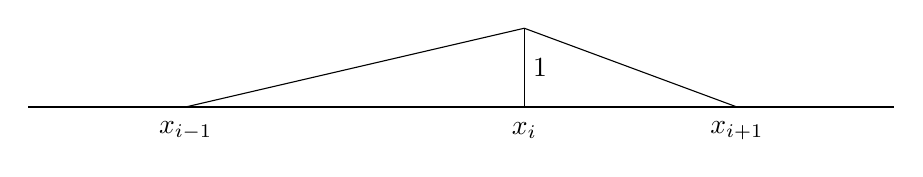
\begin{tikzpicture}[scale=1]
        % 定义三角形的三个顶点
        \draw (-5,0) -- (-3,0) -- (1.3,0) -- (4,0) -- (6,0);
        \draw (1.3,1) -- (1.3,0);
        \draw (1.3,1) -- (4,0);
        \draw (1.3,1) -- (-3,0);
        \node at (-3,-0.3) {$ x_{i-1} $};
        \node at (1.3,-0.3) {$ x_i $};
        \node at (4,-0.3) {$ x_{i+1} $};
        \node at (1.5,0.5) {$ 1 $};
    \end{tikzpicture}
    \caption{$ i $th分段线性基函数$ \phi_i $}
    \label{fig:linear_basis}
\end{figure}
\newline
令
\[
    \varphi_i(x) = 
    \begin{cases}
        \dfrac{1}{x_i-x_{i-1}}, & x\in [x_{i-1},x_i],\\
        -\dfrac{1}{x_{i+1}-x_i}, & x\in (x_i,x_{i+1}],\\
        0, & \text{otherwise},
    \end{cases}
\]
不难验证
\[
    \int_0^1 \phi_i(x) v'(x)\ dx = \left( \int_0^{x_{i-1}} + \int_{x_{i-1}}^{x_i} + \int_{x_i}^{x_{i+1}}+\int_{x_{i+1}}^1 \right)  \phi_i(x) v'(x)\ dx = - \int_0^1 \varphi_i(x) v(x)\ dx,\quad \forall v\in H^1_0(I),
\]
所以$ \varphi_i\in L^2(0,1) $是$ \phi_i $的弱导数,因此,$ \phi_i\in H^1_0(0,1) $,所以$ V_h\subset V=H^1_0(0,1) $是一个$ N $维子空间。实际上,三元组$ (I_i,\mathcal{P}_i={\rm span}\{\phi_{i-1},\phi_i\},\mathcal{N}_i=\{N_{i-1},N_i\}) $构成了一个\emph{有限元},其中$ N_i(v) = v(x_i),\ v\in \mathcal{P}_i $。当$ N_i(v) = 0 $且$ N_{i-1}(v) = 0 $时,不难看出如果$ v\in \mathcal{P}_i $则$ v=0 $,因此局部插值算子$ \mathcal{I}_i:v\in V\mapsto N_{i-1}(v)\phi_{i-1}+N_i(v)\phi_i\in \mathcal{P}_i $是良好定义的\footnote{即如果$ w_1=\mathcal{I}_i v $,$ w_2 = \mathcal{I}_i v $,则$ w_1=w_2\in \mathcal{P}_i $}。稍后为了估计有限元解的误差,需要使用到这一局部插值算子。接下来我们考虑整个区域$ I $上的情况,设$ h = \max_{i=1,\cdots ,n}|x_{i-1}-x_i| $,因为边界为齐次Dirichlet边界,因此只需考虑内部节点,令
\[
    V_h = \{v\in C^0(0,1): v|_{I_i}\in \mathcal{P}_i,\ i=1,2,\cdots ,N-1\},
\]
则$ V_h $是$ V=H^1_0(U) $的$ N-1 $维子空间。在$ V_h $上的任意函数$ v_h $都可以表示为
\begin{equation}
    v_h(x) = \sum_{i=1}^{N-1} U_i\phi_i(x),
\end{equation}
基于这一表示问题转化为$ (V_h') $形式:
\begin{equation}
    \text{Find } U\in \mathbb{R}^n \text{ such that } \sum_{i=1}^{N-1}a(\phi_i,\phi_j)U_i = l(\phi_j),\quad j=1,2,\cdots ,N-1.
\end{equation}

注意:弱解$ u\in V $在局部插值算子下的像$ \mathcal{I}_K u $尽管属于$ V_h $但是不一定满足变分关系:$ a(\mathcal{I}_K u, v_h) = l(v_h) $,因此$ \mathcal{I}_K u $不一定是有限元解。有限元解和$ \mathcal{I}_K u $都形如
\begin{equation}
    u_h(x) = \sum_{i=1}^{N-1} U_i\phi_i(x),\quad \mathcal{I}_K u(x) = \sum_{i=1}^{N-1} N_{i}(u)\psi_{i}(x),
\end{equation}
区别在于有限元解的系数$ U_i $通过变分关系确定,而$ \mathcal{I}_K u $的系数$ N_i(u) $由有限元上的局部插值算子自身给出,与问题无关,而且使用的基函数$ \psi_i $不一定和有限元解中的$ \phi_i $相同。
\paragraph*{二维问题}
接下来我们讨论稍复杂一些的二维问题,考虑一般的具有多边形边界$ \partial U $的有界区域$ U\subset \mathbb{R}^2 $上的Poisson方程齐次Dirichlet边值问题$ (D) $:
\begin{equation}
    \begin{aligned}
        -\Delta u &= f,\quad x\in U,\\
        u &= 0,\quad x\in \partial U,
    \end{aligned}
\end{equation}
这一问题的变分形式$ (V) $为:寻找$ u\in H^1_0(U) $使得
\begin{equation}
    a(u,v)=\int_U \nabla u\cdot \nabla v\ d x = \int_U fv\ d x=l(v),\quad \forall v\in H^1_0(U).
\end{equation}
为了数值求解问题$ (V) $需要将区域$ U $进行细分,这里我们使用最简单的三角剖分,如图\ref{fig:triangulation}所示。
\begin{figure}[htpb]
    \centering
    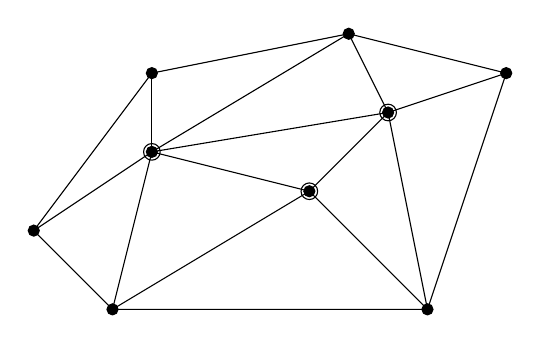
\begin{tikzpicture}
        \draw (0,0) -- (1,-1) -- (5,-1) -- (6,2) -- (4,2.5) -- (1.5,2) -- (0,0);
        \filldraw [black] (0,0) circle (2pt);
        \filldraw [black] (1,-1) circle (2pt);
        \filldraw [black] (5,-1) circle (2pt);
        \filldraw [black] (6,2) circle (2pt);
        \filldraw [black] (4,2.5) circle (2pt);
        \filldraw [black] (1.5,2) circle (2pt);
        
        \filldraw [black] (1.5,1) circle (2pt);
        \filldraw [black] (3.5,0.5) circle (2pt);
        \filldraw [black] (4.5,1.5) circle (2pt);
        \draw (1.5,1) circle (3pt);
        \draw (3.5,0.5) circle (3pt);
        \draw (4.5,1.5) circle (3pt);

        \draw (1.5,1) -- (0,0);
        \draw (1.5,1) -- (1,-1);
        \draw (1.5,1) -- (1.5,2);
        \draw (1.5,1) -- (3.5,0.5);
        \draw (1.5,1) -- (4.5,1.5);
        \draw (1.5,1) -- (4,2.5);
        \draw (3.5,0.5) -- (4.5,1.5);
        \draw (3.5,0.5) -- (1,-1);
        \draw (3.5,0.5) -- (5,-1);
        \draw (4.5,1.5) -- (4,2.5);
        \draw (4.5,1.5) -- (5,-1);
        \draw (4.5,1.5) -- (6,2);
    \end{tikzpicture}
    \caption{多边形区域的三角剖分,区分内点和节点}
    \label{fig:triangulation}
\end{figure}

记上述三角剖分为$ \mathcal{T} $,设$ h_K $为$ \mathcal{T} $中的任意三角形记为$ K $的直径,即$ h_K = \max_{x,y\in K}|x-y| $,令$ h = \max_{K\in \mathcal{T}}h_K $。在细分的每个内点(图\ref{fig:triangulation}中的带有圆圈的实心黑点)处,定义一个相应的分片线性基函数$ \phi_i $满足在该内点处为$ 1 $,在其他节点处为$ 0 $。设细分$ \mathcal{T} $的内点集为$ \{x_i\}_{i=1}^{N(h)} $,则相应地可以定义$ N(h) $个分片线性函数$ \{\phi_i\}_{i=1}^{N(h)} $,这些函数张成了$ V=H^1_0(U) $的一个$ N(h) $维的有限维空间$ V_h $:
\begin{equation}
    V_h = {\rm span}\{\phi_1,\phi_2,\cdots ,\phi_{N(h)}\}.
\end{equation}
至此我们可得有限元问题$ (V_h) $:
\begin{equation}
    \text{Find } u_h\in V_h \text{ such that } a(u_h,v_h) = l(v_h),\quad \forall v_h\in V_h.
\end{equation}
因为$ V_h $是$ V $的有限维子空间,所以$ u_h $可以表示为
\begin{equation}
    u_h(x) = \sum_{i=1}^{N(h)} U_i\phi_i(x),
\end{equation}
于是问题$ (V) $转化为问题$ (V_h') $:
\begin{equation}
    \text{Find } U\in \mathbb{R}^{N(h)} \text{ such that } \sum_{i=1}^{N(h)} a(\phi_i,\phi_j)U_i = l(\phi_j),\quad j=1,2,\cdots ,N(h).
\end{equation}

特别地,当$ U = [0,1]\times [0,1] $是正方形区域时,可以使用如图\ref{fig:triangular_on_U}所示的规则三角剖分,节点为$ (x_i,y_j) = (i,j)h $,其中$ h = 1/N $,$ i,j = 0,1,\cdots ,N $。在每个内点$ (x_i,y_j) $($ i,j=1,\cdots ,N-1 $)周围的六个三角形上(如图\ref{fig:triangular_around_node}所示),定义分片线性基函数$ \phi_{ij} $为
\begin{equation}
    \phi_{ij} = 
    \begin{cases}
        1 - \dfrac{x-x_i}{h} - \dfrac{y-y_j}{h}, & (x,y)\in K_1,\\
        1 - \dfrac{y-y_j}{h}, & (x,y)\in K_2,\\
        1 - \dfrac{x-x_i}{h}, & (x,y)\in K_3,\\
        1 + \dfrac{x-x_i}{h} + \dfrac{y-y_j}{h}, & (x,y)\in K_4,\\
        1 + \dfrac{y-y_j}{h}, & (x,y)\in K_5,\\
        1 + \dfrac{x-x_i}{h}, & (x,y)\in K_6,\\
        0, & \text{otherwise},
    \end{cases}
\end{equation}
\begin{figure}[htbp]
    \centering
    \begin{minipage}[b]{0.45\textwidth}
        \centering
        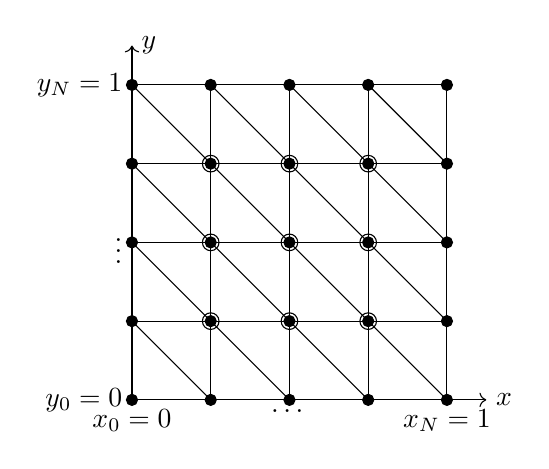
\begin{tikzpicture}
            % Draw the grid
            \draw[step=1cm] (0,0) grid (4,4);
            
            % Draw the diagonal lines in each grid square
            \foreach \x in {0,1,2,3} {
                \foreach \y in {4,3,2,1} {
                    \draw (\x,\y) -- (\x+1,\y-1);
                }
            }
            
            % Highlighted points
            \foreach \x in {0,1,2,3,4} {
                \foreach \y in {0,1,2,3,4} {
                    \draw[fill=black] (\x,\y) circle (2pt);
                }
            }
            \foreach \x in {1,2,3} {
                \foreach \y in {1,2,3} {
                    \draw (\x,\y) circle (3pt);
                }
            }
            
            % Labels on the axes
            \node[below] at (0,0) {$x_0 = 0$};
            \node[below] at (4,0) {$x_N = 1$};
            \node[left] at (0,4) {$y_N = 1$};
            \node[left] at (0,0) {$y_0 = 0$};
            \node[left] at (0,2) {$\vdots$};
            \node[below] at (2,0) {$\dots$};
            
            % Axes
            \draw[->] (0,0) -- (4.5,0) node[right] {$x$};
            \draw[->] (0,0) -- (0,4.5) node[right] {$y$};
        
        \end{tikzpicture}
        \caption{矩形区域的剖分}
        \label{fig:triangular_on_U}
    \end{minipage}
    \hfill
    \begin{minipage}[b]{0.45\textwidth}
        \centering
        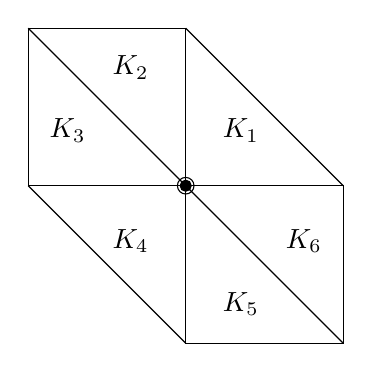
\begin{tikzpicture}[scale=1]
            \draw (0,0) -- (2,0) -- (2,-2) -- (0,-2) -- (0,2) -- (-2,2) -- (-2,0) -- (0,0);
            \draw (-2,2) -- (2,-2);
            \draw (0,2) -- (2,0);
            \draw (-2,0) -- (0,-2);
            \filldraw[black] (0,0) circle (2pt);
            \draw (0,0) circle (3pt);
            \node at (0.7,0.7) {$ K_1 $};
            \node at (-0.7,1.5) {$ K_2 $};
            \node at (-1.5,0.7) {$ K_3 $};
            \node at (-0.7,-0.7) {$ K_4 $};
            \node at (0.7,-1.5) {$ K_5 $};
            \node at (1.5,-0.7) {$ K_6 $};
        \end{tikzpicture}
        \caption{内点周围的三角剖分}
        \label{fig:triangular_around_node}
    \end{minipage}
\end{figure}

令
\[
    \varphi_{ij}^{(1)}(x,y) = 
    \begin{cases}
        -\frac{1}{h}, & (x,y)\in K_1,\\
        0, & (x,y)\in K_2,\\
        \frac{1}{h}, & (x,y)\in K_3,\\
        \frac{1}{h}, & (x,y)\in K_4,\\
        0, & (x,y)\in K_5,\\
        -\frac{1}{h}, & (x,y)\in K_6,\\
        0, & \text{otherwise},
    \end{cases}\qquad
    \varphi_{ij}^{(2)}(x,y) =
    \begin{cases}
        -\frac{1}{h}, & (x,y)\in K_1,\\
        -\frac{1}{h}, & (x,y)\in K_2,\\
        0, & (x,y)\in K_3,\\
        \frac{1}{h}, & (x,y)\in K_4,\\
        \frac{1}{h}, & (x,y)\in K_5,\\
        0, & (x,y)\in K_6,\\
        0, & \text{otherwise},
    \end{cases}
\]
可以验证$ D\phi_{ij}=(\varphi^{(1)}_{ij},\varphi^{(2)}_{ij}) $是$ \phi_{ij} $的弱导数。因为$ D\phi_{ij}\in L^2(U) $,所以$ \phi_{ij}\in H^1_0(U) $。因此,$ V_h\subset V=H^1_0(U) $是一个$ (N-1)^2 $维子空间,设
\[
    u_h(x,y) = \sum_{i=1}^{N-1}\sum_{j=1}^{N-1} U_{ij}\phi_{ij}(x,y),
\]
进而可以得到问题$ (V_h') $:
\begin{equation}
    \text{Find } U\in \mathbb{R}^{(N-1)^2} \text{ such that } \sum_{i=1}^{N-1}\sum_{j=1}^{N-1}a(\phi_{ij},\phi_{k\ell})U_{ij} = l(\phi_{k\ell}),\quad k,\ell=1,2,\cdots ,N-1.
\end{equation}
带入$ a(\phi_{ij},\phi_{k\ell}) $和$ l(\phi_{k\ell}) $的表达式,注意到$ a(\phi_{ij},\phi_{k\ell}) $只在$ (i,j) $和$ (k,\ell) $相邻时不为零,因此上式变为
\begin{equation}
    -\frac{U_{k+1,\ell}-2U_{k\ell}+U_{k-1,\ell}}{h^2} - \frac{U_{k,\ell+1}-2U_{k\ell}+U_{k,\ell-1}}{h^2} = \frac{1}{h^2}\iint_{{\rm supp}\ \phi_{k\ell}}f(x,y)\phi_{k\ell}(x,y)\ dxdy,
\end{equation}
其中$ k,\ell = 1,2,\cdots ,N-1 $,因此这种方法类似于有限差分法中的五点差分格式。

\subsection{矩阵形式\texorpdfstring{$(V_h')$}{}}
这一节我们以Poisson方程为例,展示如何将有限元问题$ (V_h') $转化为矩阵形式。考虑有界多边形区域上的二维Poisson方程齐次Dirichlet边值问题$ (D) $:
\begin{equation}
    \begin{aligned}
        -\Delta u &= f,\quad x\in U,\\
        u &= 0,\quad x\in \partial U,
    \end{aligned}
\end{equation}
该问题自伴随,因此变分问题$ (V) $等价于最优化问题$ (M) $:
\begin{equation}
    \text{Find } u\in H^1_0(U) \text{ such that } J(u) = \frac{1}{2}a(u,u) - l(u) \text{ is minimized},
\end{equation}
于是只需在$ V_h $内最小化
\[
    J(v_h) = \frac{1}{2}\int_U \nabla v_h\cdot \nabla v_h\ d x - \int_U fv_h\ d x,\quad v_h\in V_h.
\]
因为$ v_h\in V_h $,令
\[
    v_h = \sum_{i=1}^{N(h)} V_i\phi_i,
\]
其中$ \{\phi_i\}_{i=1}^{N(h)} $是$ V_h $的一组基函数,于是
\[
    a(v_h,v_h) = \sum_{i=1}^{N(h)}\sum_{j=1}^{N(h)} V_ia(\phi_i,\phi_j)V_j,\quad l(v_h) = \sum_{i=1}^{N(h)}V_il(\phi_i),
\]
因此优化问题的矩阵形式为
\begin{equation}
    \text{Find } U\in \mathbb{R}^{N(h)} \text{ such that } \frac{1}{2}V^T A V - V^T F \text{ is minimized},
\end{equation}
其中$ V = (V_1,\cdots ,V_{N(h)})^T $,$ A $是刚度矩阵,$ F $是载荷向量,满足
\[
    A_{ij} = a(\phi_i,\phi_j),\quad F_i = l(\phi_i),\quad i,j=1,2,\cdots ,N(h).  
\]
当且仅当第$ i $和第$ j $个内点是同一个三角形的顶点时$ A_{ij}\ne 0 $。因为一般情况下三角形$ K $一般标准的,为了计算$ A $和$ F $,通常需要借助仿射变换。考虑细分中的某三角形区域$ K $,它的三个顶点分别为
\[
    \bm{r}_i = (x_i,y_i),\quad i=1,2,3,
\]
令$ \bm{r} = (x,y) $为平面上的标准坐标。现在令
\begin{equation}
    \begin{aligned}
        \bm{r}(\xi,\eta) 
        &= (1-\xi-\eta)\bm{r}_1 + \xi\bm{r}_2 + \eta\bm{r}_3\\
        &= \psi_1(\xi,\eta) \bm{r}_1 + \psi_2(\xi,\eta) \bm{r}_2 + \psi_3(\xi,\eta) \bm{r}_3,
    \end{aligned}
\end{equation}
即
\begin{equation}
    \begin{aligned}
        x &= (1-\xi-\eta)x_1 + \xi x_2 + \eta x_3,\\
        y &= (1-\xi-\eta)y_1 + \xi y_2 + \eta y_3,
    \end{aligned}
\end{equation}
于是$ \bm{r} = \bm{r}(\xi,\eta) $为新的$ \xi\eta $平面上的参数表示,其中$ \psi_1,\psi_2,\psi_3 $是该局部坐标上线性函数的一组节点基($ \psi_i = \bm{r}^* \phi_i $)。

\begin{figure}[htpb]
    \centering
    \begin{tikzpicture}
        \draw[->,gray] (6,0) -- (8.5,0) node[right] {$\xi$};
        \draw[->,gray] (7,-1) -- (7,1.5) node[right] {$\eta$};
        \draw (0,0) -- (3,0) -- (1,1) -- (0,0);
        \draw (7,0) -- (8,0) -- (7,1) -- (7,0);
        \draw[<-] (4,0.5) -- (5.5,0.5);
        \node at (4.75,0.7) {$ \bm{r} $};
        \node at (1,0.5) {$ K $};
        \node at (6.75,1) {$ 1 $};
        \node at (8,-0.25) {$ 1 $};
    \end{tikzpicture}
    \caption{线性变换$ \bm{r} $将一般的三角形$ K $拉回到标准三角形}
    \label{fig:triangle_tran}
\end{figure}

线性变换$ (\xi,\eta)\mapsto \bm{r} = (x,y) $的Jacobi矩阵为
\begin{equation}
    J = \dfrac{\partial (x,y)}{\partial (\xi,\eta)} =
    \begin{pmatrix}
        \frac{\partial x}{\partial \xi} & \frac{\partial x}{\partial \eta}\\
        \frac{\partial y}{\partial \xi} & \frac{\partial y}{\partial \eta}
    \end{pmatrix} = 
    \begin{pmatrix}
        x_2-x_1 & x_3-x_1\\
        y_2-y_1 & y_3-y_1
    \end{pmatrix},
\end{equation}
不难发现
\[
    |J| = \det \begin{pmatrix} 
        x_2-x_1 & x_3-x_1\\
        y_2-y_1 & y_3-y_1
    \end{pmatrix} = 
    \begin{vmatrix}
        x_1 & x_2 & x_3\\
        y_1 & y_2 & y_3\\
        1 & 1 & 1
    \end{vmatrix} = 2S_K,
\]
其中$ S_K $是三角形$ K $的面积。于是对于$ K $上的任意$ v_h\in V_h $,借助$ v_h $的线性性可知
\begin{equation}
    v_h(x,y) = v_h(\bm{r}(\xi,\eta)) = v_h(\xi,\eta) = V_1 \psi_1(\xi,\eta) + V_2 \psi_2(\xi,\eta) + V_3 \psi_3(\xi,\eta),
\end{equation}
其中$ V_i = v_h(r_i) $,带入$ \psi_i $的定义可知
\[
    \dfrac{\partial v_h}{\partial \xi} = V_2 - V_1,\quad \dfrac{\partial v_h}{\partial \eta} = V_3 - V_1.
\]
另一方面,使用链式法则对$ v_h $关于$ x,y $求偏导可得
\begin{equation}
    \begin{pmatrix} 
        \frac{\partial v_h}{\partial \xi}  \\ \frac{\partial v_h}{\partial \eta} 
    \end{pmatrix} = 
    \begin{pmatrix} 
        \frac{\partial x}{\partial \xi} & \frac{\partial y}{\partial \xi} \\
        \frac{\partial x}{\partial \eta} & \frac{\partial y}{\partial \eta}
    \end{pmatrix}
    \begin{pmatrix} 
        \frac{\partial v_h}{\partial x}  \\ \frac{\partial v_h}{\partial y}
    \end{pmatrix} = J^T 
    \begin{pmatrix} 
        \frac{\partial v_h}{\partial x}  \\ \frac{\partial v_h}{\partial y}
    \end{pmatrix},
\end{equation}
于是(对角元互换,非对角元变为相反数)
\begin{equation}
    \begin{aligned}
        \nabla v_h = \begin{pmatrix} \frac{\partial v_h}{\partial x} \\ \frac{\partial v_h}{\partial y} \end{pmatrix} = J^{-T} \begin{pmatrix} \frac{\partial v_h}{\partial \xi} \\ \frac{\partial v_h}{\partial \eta} \end{pmatrix} 
        = \frac{1}{|J|}
        \begin{bmatrix} 
            y_3-y_1 & -(y_2-y_1)\\
            -(x_3-x_1) & x_2-x_1     
        \end{bmatrix} 
        \begin{pmatrix} 
            \frac{\partial v_h}{\partial \xi} \\ \frac{\partial v_h}{\partial \eta}
        \end{pmatrix},
    \end{aligned}
\end{equation}
进而
\begin{equation}
    |J|^2 |\nabla v_h|^2 = |\bm{r}_3-\bm{r}_1|^2 \left( \dfrac{\partial v_h}{\partial \xi} \right)^2 + |\bm{r}_2-\bm{r}_1|^2 \left( \dfrac{\partial v_h}{\partial \eta} \right)^2 - 2(\bm{r}_3-\bm{r}_1)\cdot (\bm{r}_2-\bm{r}_1)\dfrac{\partial v_h}{\partial \xi}\dfrac{\partial v_h}{\partial \eta}.
\end{equation}
带入$ \partial v_h / \partial \xi = V_2 - V_1,\ \partial v_h / \partial \eta = V_3 - V_1 $,于是上式变为
\[
    \begin{aligned}
        |J|^2 |\nabla v_h|^2 
        &= [|\bm{r}_3-\bm{r}_1|^2+|\bm{r}_2-\bm{r}_1|^2- 2(\bm{r}_3-\bm{r}_1)\cdot (\bm{r}_2-\bm{r}_1)]V_1^2 \\
        &+ |\bm{r}_3-\bm{r}_1|^2V_2^2 + |\bm{r}_2-\bm{r}_1|^2V_3^2 - 2(\bm{r}_3-\bm{r}_1)\cdot (\bm{r}_2-\bm{r}_1)V_2V_3 \\
        &+ [-2|\bm{r}_3-\bm{r}_1|^2+2(\bm{r}_3-\bm{r}_1)\cdot (\bm{r}_2-\bm{r}_1)]V_1V_2 + [-2|\bm{r}_2-\bm{r}_1|^2+2(\bm{r}_3-\bm{r}_1)\cdot (\bm{r}_2-\bm{r}_1)]V_1V_3.
    \end{aligned}
\]
根据余弦定理
\[
    |\bm{r}_3-\bm{r}_1|^2+|\bm{r}_2-\bm{r}_1|^2- 2(\bm{r}_3-\bm{r}_1)\cdot (\bm{r}_2-\bm{r}_1) = |\bm{r}_3-\bm{r}_2|^2,
\]
另一方面
\[
    -2|\bm{r}_3-\bm{r}_1|^2+2(\bm{r}_3-\bm{r}_1)\cdot (\bm{r}_2-\bm{r}_1) = 2(\bm{r}_2-\bm{r}_3)\cdot (\bm{r}_3-\bm{r}_1),
\]
所以
\[
    \begin{aligned}
        |J|^2 |\nabla v_h|^2 
        &= |\bm{r}_3-\bm{r}_2|^2V_1^2 + |\bm{r}_3-\bm{r}_1|^2V_2^2 + |\bm{r}_2-\bm{r}_1|^2V_3^2 - 2(\bm{r}_3-\bm{r}_1)\cdot (\bm{r}_2-\bm{r}_1)V_2V_3 \\
        &+ 2(\bm{r}_2-\bm{r}_3)\cdot (\bm{r}_3-\bm{r}_1)V_1V_2 + 2(\bm{r}_1-\bm{r}_2)\cdot (\bm{r}_2-\bm{r}_3)V_1V_3.
    \end{aligned}
\]
注意到$ v_h $在$ K $上是线性函数,因此$ \nabla v_h $在$ K $上不会发生变化,于是
\begin{equation}
    \int_K |\nabla v_h(x,y)|^2dxdy = S_K |\nabla v_h|^2,
\end{equation}
所以
\[
    \int_K |\nabla v_h(x,y)|^2dxdy = \frac{1}{4S_K}|J|^2 |\nabla v_h|^2 = \frac{1}{4S_K} [V_1,V_2,V_3]A^{(K)} \begin{bmatrix} 
        V_1 \\ V_2\\ V_3, 
    \end{bmatrix} 
\]
其中
\[
    A^{(K)}=\begin{bmatrix} 
        |\bm{r}_2-\bm{r}_3|^2 & (\bm{r}_2-\bm{r}_3)\cdot (\bm{r}_3-\bm{r}_1) & (\bm{r}_2-\bm{r}_3)\cdot (\bm{r}_1-\bm{r}_2)\\
         & |\bm{r}_3-\bm{r}_1|^2 & (\bm{r}_3-\bm{r}_1)\cdot (\bm{r}_1-\bm{r}_2)\\
        \text{symm.}    & & |\bm{r}_1-\bm{r}_2|^2
    \end{bmatrix}
\]
是对称矩阵。由于
\[
    a(v_h,v_h) = \sum_{K\in \mathcal{T}}\int_K |\nabla v_h(x,y)|^2dxdy = \sum_{K\in \mathcal{T}}\frac{1}{4S_K} [V^{(K)}_1,V^{(K)}_2,V^{(K)}_3]A^{(K)} \begin{bmatrix} 
        V^{(K)}_1 \\ V^{(K)}_2\\ V^{(K)}_3,
    \end{bmatrix},
\]
所以可以使用$ A^{(K)} $来组装刚度矩阵$ A $。对细分$ \mathcal{T} $的节点进行编号,不妨将内点排列到边界点的前面,令前$ N_1(h) $个节点为内点,后$ N_2(h) $个节点为边界点,于是
\[
    u_h = \sum_{i=1}^{N_1(h)} U_i\phi_i + \sum_{i=N_1(h)+1}^{N(h)} U_i\phi_i,
\]
其中$ \phi_i $是在第$ i $个格点处为$ 1 $,在其他格点处为$ 0 $的分片线性函数。因为边界为齐次Dirichlet边界,所以$ U_{N_2(h)+1} = U_{N_2(h)+2} = \cdots = U_{N(h)} = 0 $,因此
\[
    u_h = \sum_{i=1}^{N_1(h)} U_i\phi_i.
\]
考虑任意$ K\in \mathcal{T} $,令$ L^{(K)} $为一个只以$ 0,1 $为元素的$ N(h)\times 3 $阶矩阵,如果$ K $的三个顶点向量$ \bm{r}_1,\bm{r}_2,\bm{r}_3 $分别对应第$ i,j,k $个节点,则
\[
    L^{(K)}_{i1} = L^{(K)}_{j2} = L^{(K)}_{k3} = 1,
\]
其他元素均为$ 0 $。现在令
\begin{equation}
    A^* = \sum_{K\in \mathcal{T}} L^{(K)} A^{(K)} (L^{(K)})^T
\end{equation}
称为完全刚度矩阵,类似地可以构造完全载荷向量$ F^* $。分别删去$ A^* $的后$ N_2(h) $行和列以及$ F^* $的后$ N_2(h) $个元素得到$ A $和$ F $,至此得到了有限元问题$ (V_h') $的矩阵形式:
\begin{equation}
    AU = F.
\end{equation}

如果细分足够好的话,$ \phi_i $比较容易计算和积分,则可以直接计算$ a(\phi_i,\phi_j) $和$ l(\phi_i) $。如果使用分片多项式函数而非线性函数,则需要进行数值积分。

\subsection{先验误差估计}
下面我们估计线性有限元方法的误差。设问题仍然为形如\eqref{eq:elliptic_Dirichlet}的线性二阶椭圆方程的齐次Dirichlet边值问题$ (D) $,相应的有限元问题$ (V_h) $为
\begin{equation}\label{eq:finite_element}
    \text{Find } u_h\in V_h \text{ such that } a(u_h,v_h) = l(v_h),\quad \forall v_h\in V_h,
\end{equation}
注意到$ V_h\subset V $,根据弱解的定义,$ (V) $的解$ u $满足
\[
    a(u,v) = l(v),\quad \forall v\in V,
\]
所以
\begin{equation}\label{eq:weak_solution_in_Vh}
    a(u,v_h) = l(v_h),\quad \forall v_h\in V_h,
\end{equation}
将\eqref{eq:finite_element}与\eqref{eq:weak_solution_in_Vh}相减,得到
\begin{equation}\label{eq:Galerkin_orthogonality}
    a(u-u_h,v_h) = 0,\quad \forall v_h\in V_h,
\end{equation}
因此插值误差$ u-u_h $与$ V_h $在$ a(\cdot,\cdot) $下正交,这一性质称为\emph{Galerkin正交性}(Galerkin orthogonality)。

\subsubsection{Céa引理}
通过利用Galerkin正交性和椭圆问题本身的性质可以得到有限元解$ u_h $与原问题解$ u $之间的误差估计。
\begin{lemma}{\normalfont\bf{(Céa)}}\label{lemma:Cea}
    如果$ u_h $为问题$ (V_h) $的解,即弱解$ u\in V=H^1_0(U) $的有限元逼近,则在范数$ \| \cdot \|_{H^1(U)} $下,$ u_h $是$ u $在有限维空间$ V_h $内的几乎最优逼近,即
    \begin{equation}\label{eq:Cea}
        \| u-u_h \|_{H^1(U)} \leqslant \frac{c_1}{c_0}\inf_{v_h\in V_h}\| u-v_h \|_{H^1(U)}.
    \end{equation}
\end{lemma}
\begin{proof}
    根据之前的分析,当\eqref{eq:elliptic_inequality}时,$ a(\cdot,\cdot) $是椭圆的,即存在$ c_0>0 $使得
    \[
        c_0\| v \|_{H^1(U)}^2 \leqslant a(v,v),\quad \forall v\in V.
    \]
    因为$ u_h\in V_h\subset V $,所以$ u_h-u\in V $,于是
    \[
        \| u_h-u \|_{H^1(U)}^2 \leqslant \frac{1}{c_0}a(u_h-u,u_h-u).
    \]
    又因为插值误差$ u-u_h $与$ V_h $在$ a(\cdot,\cdot) $下正交,即\eqref{eq:Galerkin_orthogonality}成立,而$ v_h\in V_h $时$ u_h-v_h\in V_h $,所以
    \[
        a(u_h-u,u_h-u) = a(u_h-u,v_h-u) + a(u_h-u,u_h-v_h) = a(u_h-u,v_h-u),\quad \forall v_h\in V_h,
    \]
    进而
    \[
        \| u_h-u \|_{H^1(U)}^2 \leqslant \frac{1}{c_0}a(u_h-u,v_h-u),\quad \forall v_h\in V_h.
    \]
    接着再使用$ a $的有界性可知存在$ c_1>0 $使得
    \[
        \| u_h-u \|_{H^1(U)}^2 \leqslant \frac{c_1}{c_0}\| u_h-u \|_{H^1(U)}\| v_h-u \|_{H^1(U)},\quad \forall v_h\in V_h,
    \]
    两边同时除以$ \| u_h-u \|_{H^1(U)} $即可得到引理的结论。
\end{proof}

一般地,逼近函数可以不局限于线性函数,在下一章我们将介绍以分片多项式作为形状函数的有限元方法,对于这类方法我们有一般性的结论:
\begin{equation}
    \inf_{v_h\in V_h}\| u-v_h \|_{H^1(U)} \leqslant C(u)h^s,
\end{equation}
其中$ C(u)>0 $是一个与$ u $的光滑性有关的常数,$ h $是细分的最大直径,$ s $与使用的多项式阶数和$ u $的光滑性有关,当使用线性元时$ s=1 $。将上式带入Céa引理中可以得到
\begin{equation}\label{eq:Cea_general}
    \| u-u_h \|_{H^1(U)} \leqslant \frac{c_1}{c_0}C(u)h^s.
\end{equation}
\begin{example}
    考虑$ \mathbb{R}^n $上对流扩散方程的齐次Dirichlet边值问题$ (D) $:
    \begin{equation}
        \begin{aligned}
            -\epsilon \Delta u + \bm{b}\cdot\nabla u &= f,\quad x\in U,\\
            u &= 0,\quad x\in \partial U,
        \end{aligned}
    \end{equation}
    其中$ \bm{b}=(b_1,\cdots ,b_n) $,$ b_i\in W^{1,\infty}(U) $。要求$ \epsilon>0 $以保证该问题适定。为了简单起见要求$ \nabla b_i\leqslant 0 $在$ U $上几乎处处成立。现在我们考虑使用分片线性有限元方法得到的有限元解与真实解之前的误差。

    该问题相应的变分问题$ (V) $为:寻找$ u\in V=H^1_0(U) $使得
    \begin{equation}
        a(u,v) = \int_U \epsilon \nabla u\cdot \nabla v + \bm{b}\cdot\nabla u v\ d x = \int_U fv\ d x = l(v),\quad \forall v\in V.
    \end{equation}
    其中
    \[
        a(u,v) = \int_U \epsilon \nabla u\cdot \nabla v + \bm{b}\cdot\nabla u v\ d x,\quad l(v) = \int_U fv\ d x.
    \]
    因此问题满足一致椭圆性条件
    \[
        \sum_{i,j=1}^n (\epsilon \delta_{ij}) \xi_i\xi_j = \epsilon \sum_{i=1}\xi_i^2,\quad \forall \bm{\xi}\in \mathbb{R}^n,
    \]
    所以$ \tilde{c}=\epsilon $。令$ c^* $为Poincaré不等式中的常数,即
    \[
        c^* = \inf_{v\in V=H^1_0(U)}\frac{\| \nabla v \|_{L^2(U)}}{\| v \|_{L^2(U)}}.
    \]
    根据之前的分析,\eqref{eq:elliptic_inequality}成立时,$ a(\cdot,\cdot) $是椭圆的,存在$ c_0>0 $使得
    \[
        c_0\| v \|_{H^1(U)}^2 \leqslant a(v,v),\quad \forall v\in V.
    \]
    其中
    \begin{equation}
        c_0 = \frac{\tilde{c}}{1+c^*} = \frac{\epsilon}{1+c^*}.
    \end{equation}
    另一方面,考虑$ a(\cdot,\cdot) $的有界性。由Cauchy-Schwarz不等式可得
    \[
        \begin{aligned}
            |a(v,w)| \leqslant \epsilon \| \nabla v \|_{L^2(U)}\| \nabla w \|_{L^2(U)} + \left| \int_U \bm{b}\cdot \nabla vw\ d x  \right| .
        \end{aligned}
    \]
    使用Hölder不等式\footnote{$ 1\leqslant p,q\leqslant \infty $且$ \frac{1}{p}+\frac{1}{q}=1 $时,如果$ f\in L^p(U),g\in L^q(U) $,则$ \| fg \|_{L^1(U)} \leqslant \| f \|_{L^p(U)} \| g \|_{L^q(U)} $}和均值不等式可得
    \[
        \begin{aligned}
            \left| \int_U \bm{b}\cdot \nabla vw\ d x  \right| 
            &\leqslant \| |\bm{b}| \|_{L^\infty(U)} \| \nabla v \|_{L^2(U)} \| w \|_{L^2(U)}\\
            &\leqslant \| |\bm{b}| \|_{L^\infty(U)} \| v \|_{H^1(U)} \| w \|_{H^1(U)},
        \end{aligned}
    \]
    于是
    \[
        \begin{aligned}
            |a(v,w)|
            &\leqslant \epsilon \| \nabla v \|_{L^2(U)}\| \nabla w \|_{L^2(U)} + \| |\bm{b}| \|_{L^\infty(U)} \| v \|_{H^1(U)} \| w \|_{H^1(U)}\\
            &\leqslant \left( \epsilon + \| |\bm{b}| \|_{L^\infty(U)} \right) \|_{L^\infty(U)} \| v \|_{H^1(U)} \| w \|_{H^1(U)}\\
            &\leqslant \left( \epsilon^2 + \sum_{i=1}^n\| b_i \|^2_{L^\infty(U)} \right)^{1 / 2}  \| v \|_{H^1(U)} \| w \|_{H^1(U)},
        \end{aligned}
    \]
    因此
    \begin{equation}
        c_1 = \left( \epsilon^2+\sum_{i=1}^n\| b_i \|_{L^\infty}^2  \right)^{1 / 2},
    \end{equation}
    进而根据\eqref{eq:Cea_general}有
    \begin{equation}
        \| u-u_h \|_{H^1(U)} \leqslant \frac{\left( \epsilon^2+\sum_{i=1}^n\| b_i \|_{L^\infty}^2  \right)^{1 / 2}}{\epsilon} (1+c^*) C(u) h^s.
    \end{equation}
    因为通常称
    \begin{equation}
        \frac{\left( \sum_{i=1}^n\| b_i \|_{L^\infty}^2  \right)^{1 / 2}}{\epsilon} = {\rm Pe}
    \end{equation}
    为Péclet数,所以误差估计可以写为
    \begin{equation}
        \| u-u_h \|_{H^1(U)} \leqslant (1+{\rm Pe}^2)^{1 / 2} (1+c^*) C(u) h^s.
    \end{equation}
\end{example}
上述例子中我们使用到了
\[
    \left| \int_U \bm{b}\cdot \nabla vw\ d x  \right| \leqslant \| |\bm{b}| \|_{L^\infty(U)} \| Dv \|_{L^2(U)} \| w \|_{L^2(U)},
\]
证明只需注意到
\[
    \begin{aligned}
        \text{LHS} \leqslant \sum_{i=1}^n \int_U |b_i||\dfrac{\partial v}{\partial x_i} ||w|\ d x 
        &\leqslant \sum_{i=1}^n \max_{x\in U}|b_i(x)|\int_U |\dfrac{\partial v}{\partial x_i} ||w|\ d x \\
        &\leqslant \sum_{i=1}^n \max_{x\in U}|b_i(x)| \left( \int_U |\dfrac{\partial v}{\partial x_i} |^2\ dx \right)^{\frac{1}{2}} \left(  \int_U|w|^2\ d x \right)^{\frac{1}{2}} \\
        &\leqslant \left( \sum_{i=1}^n \max_{x\in U}|b_i(x)|^2 \right)^{1 / 2} \left( \sum_{i=1}^n \int_U |\dfrac{\partial v}{\partial x_i}|^2  \right)^{\frac{1}{2}} \left( \int_U |w|^2\ d x \right)^{\frac{1}{2}}.
    \end{aligned}
\]
事实上,该例子中$ a $的强制性可以直接验证。

总的来说,Céa引理提供了一种估计有限元解的误差的手段:首先借助一个更容易估计$ \| u-Tu \|_{H^1(U)} $的$ Tu\in V_h $来得到\eqref{eq:Cea}右侧的一个上界,再使用Céa引理可知该上界也是有限元解$ u_h $的误差$ \| u-u_h \|_{H^1(U)} $的一个上界。通常选取$ Tu $为$ u $的一个插值,这类插值的误差估计相对容易得到且通常只与被插值函数的光滑性、插值函数的阶数和网格大小有关。

\subsubsection{分片线性函数插值}
为了利用Céa引理对有限元解进行误差估计,需要在$ V_h $内寻找插值函数近似$ u $并估计该插值函数的误差。本节考虑解空间$ V=H^1(U) $,有限元空间$ V_h = \{v\in V:v|_K \text{ is linear}, K\in \mathcal{T}\} $的情况。令$ h_K $为$ K $的直径,$ h = \max_{K\in \mathcal{T}}h_K $为网格的最大直径,$ \rho_K $为$ K $的内切圆直径。为了避免出现奇异性,需要要求细分的每个单元$ K $都相对较好,为此要求
\begin{equation}\label{eq:mesh_condition}
    \frac{\rho_K}{h_K} \geqslant \mu>0,\quad \forall K\in \mathcal{T},
\end{equation}
这一要求保证三角形$ K $的内角不会太小,即$ K $不能太扁。现在我们定义插值算子$ \mathcal{I}_h:C^0(\overline{U})\mapsto V_h $为
\begin{equation}
    \mathcal{I}_h v = \sum_{i=1}^{N(h)} v(z_i)\psi_i,
\end{equation}
其中$ \{z_i\} $是$ \mathcal{T} $的所有节点,$ \{\psi_i\} $是$ V_h $的一组基函数,满足$ \psi_i(z_j) = \delta_{ij} $。对于这一线性插值算子,我们有如下局部插值误差估计。
\begin{theorem}
    设$ K\in \mathcal{T} $是$ U $的三角剖分,$ z_1,z_2,z_3 $是$ K $的三个顶点。给定$ v\in C^0(K) $,定义它在$ K $上的线性插值为
    \begin{equation}
        \mathcal{I}_K v = v(z_1)\psi_1 + v(z_2)\psi_2 + v(z_3)\psi_3,
    \end{equation}
    则
    \begin{enumerate}
        \item 零阶误差估计:
        \begin{equation}
            \| v-\mathcal{I}_K v \|_{L^\infty(K)} \leqslant 2h_K^2\max_{|\alpha|=2}\| D^\alpha v \|_{L^\infty(K)},
        \end{equation}
        \item 一阶误差估计:
        \begin{equation}
            \max_{|\alpha|=1}\| D^\alpha(v-\mathcal{I}_K v) \|_{L^\infty(K)} \leqslant 6\frac{h_K^2}{\rho_K}\max_{|\alpha|=2}\| D^\alpha v \|_{L^\infty(K)},
        \end{equation}
    \end{enumerate}
    其中$ \| v \|_{L^\infty(K)} = \max_{x\in K}|v(x)| $。
\end{theorem}
\begin{proof}
    对$ v $在$ x $处进行Taylor展开可得
    \[
        v(y) = v(x) + \nabla v(x)\cdot (y-x) + R(x,y),
    \]
    其中$ R $是余项,可以表示为
    \[
        R(x,y) = \frac{1}{2} \sum_{i,j=1}^2 \dfrac{\partial^2 v}{\partial x_i \partial x_j}|_{x=\xi} (y_i-x_i)(y_j-x_j),
    \]
    其中$ \xi $位于$ x $和$ y $之间,于是当$ y=z_i $为$ K $的顶点,$ x\in K $时有
    \[
        \left\vert \dfrac{\partial^2 v}{\partial x_i \partial x_j}|_{x=\xi} \right\vert \leqslant \max_{|\alpha|=2}\| D^\alpha v \|_{L^\infty(K)},
    \]
    且$ |z_1-x|\leqslant h_K $,所以
    \begin{equation}
        R(x,z_i) \leqslant 2h_K^2 \max_{|\alpha|=2}\| D^\alpha v \|_{L^\infty(K)}.
    \end{equation}
    另一方面,因为
    \[
        v(z_i) = v(x) + \nabla v(x)\cdot (z_i-x) + R(x,z_i),
    \]
    而根据定义
    \[
        \mathcal{I}_K v = v(z_1)\psi_1 + v(z_2)\psi_2 + v(z_3)\psi_3,
    \]
    所以
    \begin{equation}
        \mathcal{I}_K v(x) = v(x)\sum_{i=1}^3 \psi_i + \nabla v(x)\cdot \sum_{i=1}^3 (z_i-x)\psi_i + \sum_{i=1}^3 R(x,z_i)\psi_i(x).
    \end{equation}
    注意到当$ v $是线性函数时,$ \mathcal{I}_K v = v $。令$ v\equiv 1 $可得$ \sum_{i=1}^3 \psi_i = 1 $;令$ v(x) = d_1x_1+d_2x_2 $可得
    \[
        \nabla v\cdot\sum_{i=1}^3 (z_i-x)\psi_i = (d_1,d_2)\cdot \sum_{i=1}^3 (z_i-x)\psi_i = 0
    \]
    对任意$ (d_1,d_2) $成立,因此
    \[
        \sum_{i=1}^3 (z_i-x)\psi_i = 0,
    \]
    于是
    \begin{equation}
        \mathcal{I}_K v(x) = v(x) + \sum_{i=1}^3 R(x,z_i)\psi_i(x),
    \end{equation}
    进而我们有
    \begin{equation}
        \begin{aligned}
            \| v-\mathcal{I}_K v \|_{L^\infty(K)} &\leqslant \max_{i=1,2,3}\max_{x\in K}|R(x,z_i)|\sum_{i=1}^3 |\psi_i(x)|\\
            &\leqslant 2h_K^2 \max_{|\alpha|=2}\| D^\alpha v \|_{L^\infty(K)}.
        \end{aligned}
    \end{equation}
    对于一阶误差估计,我们有
    \begin{equation}
        \dfrac{\partial }{\partial x_1} \mathcal{I}_K v(x) = v(z_1) \dfrac{\partial \psi_1}{\partial x_1} + v(z_2) \dfrac{\partial \psi_2}{\partial x_1} + v(z_3) \dfrac{\partial \psi_3}{\partial x_1},
    \end{equation}
    带入$ v(z_i) $在$ x $处的Taylor展开可得
    \begin{equation}
        \begin{aligned}
            \dfrac{\partial }{\partial x_1} \mathcal{I}_K v(x) &= \sum_{i=1}^3 \left( v(x)+\nabla v(x)\cdot(z_i-x) + R(x,z_i) \right) \dfrac{\partial \psi_i}{\partial x_1} \\
            &=v(x)\dfrac{\partial }{\partial x_1} \left( \sum_{i=1}^3\phi_i \right) + \nabla v(x)\cdot \sum_{i=1}^3 (z_i-x)\dfrac{\partial \psi_i}{\partial x_1} + \sum_{i=1}^3 R(x,z_i)\dfrac{\partial \psi_i}{\partial x_1},
        \end{aligned}
    \end{equation}
    因为\footnote{第二个等式仍然需要考虑线性函数$ w = d_1x_1+d_2x_2 $,此时$ \mathcal{I}_K w = w $,$ R(x,z_i)=0 $,于是$ \frac{\partial }{\partial x_j} \mathcal{I}_K w = \frac{\partial w}{\partial x_j} =w\frac{\partial }{\partial x_j} (\psi_1+\psi_2+\psi_3) + \nabla w\cdot \sum_{i=1}^3(z_i-x)\frac{\partial \psi_i}{\partial x_j} +\sum_{i=1}^3 R(x,z_i)\frac{\partial \psi_i}{\partial x_j} = (d_1,d_2) \cdot \sum_{i=1}^3(z_i-x)\frac{\partial \psi_i}{\partial x_j} $。令$ w = \frac{\partial v}{\partial x_1} x_1+ \frac{\partial v}{\partial x_2}x_2 $可得$ \frac{\partial v}{\partial x_j} =\nabla v \cdot \sum_{i=1}^3(z_i-x)\frac{\partial \psi_i}{\partial x_j} $}
    \[
        \dfrac{\partial }{\partial x_1} \left( \sum_{i=1}^3\psi_i \right) = 0,\quad\dfrac{\partial v}{\partial x_1} = \nabla v(x)\cdot \sum_{i=1}^3 (z_i-x)\dfrac{\partial \psi_i}{\partial x_1},
    \]
    所以
    \begin{equation}
        \dfrac{\partial }{\partial x_1} \mathcal{I}_K v(x) = \dfrac{\partial v}{\partial x_1} + \sum_{i=1}^3 R(x,z_i)\dfrac{\partial \psi_i}{\partial x_1},
    \end{equation}
    于是得到了一阶误差的表示
    \begin{equation}
        D^\alpha (v - \mathcal{I}_K v(x)) = - \sum_{i=1}^3 R(x,z_i)D^\alpha \psi_i.
    \end{equation}
    注意到
    \begin{equation}
        \max_{j=1,2}\max_{x\in K}\left\vert \dfrac{\partial \psi_i}{\partial x_j}(x) \right\vert \leqslant \frac{1}{\rho_K},
    \end{equation}
    于是
    \begin{equation}
        \max_{|\alpha|=1}\| D^\alpha(v-\mathcal{I}_K v) \|_{L^\infty(K)} \leqslant 6\frac{h_K^2}{\rho_K}\max_{|\alpha|=2}\| D^\alpha v \|_{L^\infty(K)},
    \end{equation}
    证毕。
\end{proof}

换用其他范数可以得到类似的结论,例如在$ L^2(K) $范数下的误差估计为
\begin{theorem}
    设$ K\in \mathcal{T} $是$ U $的三角剖分,$ z_1,z_2,z_3 $是$ K $的三个顶点。给定$ v\in C^0(K) $,定义它在$ K $上的线性插值为
    \begin{equation}
        \mathcal{I}_K v = v(z_1)\psi_1 + v(z_2)\psi_2 + v(z_3)\psi_3,
    \end{equation}
    则
    \begin{enumerate}
        \item 零阶误差估计:
        \begin{equation}
            \| v-\mathcal{I}_K v \|_{L^2(K)} \leqslant Ch_K^2 |v|_{H^2(K)},
        \end{equation}
        \item 一阶误差估计:
        \begin{equation}
            |v-\mathcal{I}_K v|_{H^1(K)} \leqslant C\frac{h_K^2}{\rho_K}|v|_{H^2(K)},
        \end{equation}
    \end{enumerate}
    其中$ |w|_{H^1(K)} = (\int_K \nabla w\cdot \nabla w)^{1 / 2} $,$ |w|_{H^2(K)} = (\sum_{|\alpha|=2}\int_K |D^\alpha w|^2)^{1 / 2} $。
\end{theorem}

在以上结论的基础上可以得到在整个区域$ U $上的全局插值误差估计。因为
\[
    \begin{aligned}
        \| u - \mathcal{I}_K u \|_{L^2(U)}^2 &= \sum_{K\in \mathcal{T}}\| u - \mathcal{I}_K u \|_{L^2(K)}^2\\
        &\leqslant C\sum_{K\in \mathcal{T}}h_K^4|u|_{H^2(K)}^2\\
        &\leqslant Ch^4|u|_{H^2(U)}^2,
    \end{aligned}
\]
因此
\begin{equation}
    \| u - \mathcal{I}_h u \|_{L^2(U)} \leqslant Ch^2|u|_{H^2(U)}.
\end{equation}
类似地,一阶误差估计为
\[
    \begin{aligned}
        |u-\mathcal{I}_h u|_{H^1(U)}^2 &= \sum_{K\in \mathcal{T}}|u-\mathcal{I}_K u|_{H^1(K)}^2\\
        &\leqslant C^2\sum_{K\in \mathcal{T}}\frac{h_K^4}{\rho_K^2}|u|_{H^2(K)}^2\\
        &\leqslant \frac{C^2}{\mu^2}h^2|u|_{H^2(U)}^2,
    \end{aligned}  
\]
所以
\begin{equation}
    |u-\mathcal{I}_h u|_{H^1(U)} \leqslant \frac{C}{\mu}h|u|_{H^2(U)}.
\end{equation}

\subsubsection{能量范数下的最优误差界}
考虑简单的Poisson方程$ -\Delta u = f $的齐次Dirichlet边值问题。由Céa引理可知此时
\[
    \| u-u_h \|_{H^1(U)} \leqslant \frac{c_1}{c_0} \inf_{v_h\in V_h}\| u-v_h \|_{H^1(U)},
\]
其中的$ c_1=c_0=1 $,注意到$ u_h\in V_h $,所以
\begin{equation}
    \| u-u_h \|_{H^1(U)} = \inf_{v_h\in V_h}\| u-v_h \|_{H^1(U)}.
\end{equation}
这说明对于Poisson方程的齐次Dirichlet边值问题,有限元解$ u_h $是$ H^1(U) $范数下在$ V_h $内的最佳逼近。对于更一般的情况,因为无法再保证$ c_1 = c_0 $,所以这一结论无法继续成立。不过,通过使用能量范数,我们将看到对于自伴随椭圆方程,有限元解$ u_h $是能量范数下在$ V_h $内的最佳逼近。

以下要求$ \mathcal{L} $是自伴随微分算子,即$ a_{ij} = a_{ji} $且$ b_j=0 $,这种情况下可以定义
\begin{equation}
    (\cdot,\cdot)_a : H^1_0(U)\times H^1_0(U)\to \mathbb{R},\quad (u,v)_a = a(u,v)
\end{equation}
为Hilbert空间$ H^1(U) $上的新的内积,相应地诱导出\emph{能量范数}
\begin{equation}
    \| u \|_a = (u,u)_a^{1 / 2} = a(u,u)^{1 / 2}.
\end{equation}
根据强制性,$ a(v,v)\geqslant c_0 \| v \|^2_{H^1(U)} $,即$ \| v \|_a\geqslant \sqrt{c_0} \| v \|_{H^1(U)} $;根据椭圆性,$ a(v,v)\leqslant c_1 \| v \|_{H^1(U)}^2 $,即$ \| v \|_a\leqslant \sqrt{c_1} \| v \|_{H^1(U)} $。因此$ \| \cdot \|_a $与$ \| \cdot \|_{H^1(U)} $等价,即
\begin{equation}
    \sqrt{c_0} \| v \|_{H^1(U)} \leqslant \| v \|_a \leqslant \sqrt{c_1} \| v \|_{H^1(U)}.
\end{equation}

根据Galerkin正交性,有限元解$ u_h $满足
\begin{equation}
    a(u-u_h,v_h) = 0,\quad \forall v_h\in V_h,
\end{equation}
此即$ (u-u_h,v_h)_a = 0 $。现在考虑$ u-u_h $的能量范数,令$ v_h $是任意的$ V_h $中的函数,有
\[
    \begin{aligned}
        \| u-u_h \|_a^2 = a(u-u_h,u-u_h) 
        &= a(u-u_h,u-v_h+v_h-u_h)\\
        &= a(u-u_h,u-v_h) + a(u-u_h,v_h-u_h)\\
        &= (u-u_h,u-v_h)_a\\
        &\leqslant \| u-u_h \|_a \| u-v_h \|_a,
    \end{aligned}
\]
其中最后一步使用Cauchy-Schwarz不等式而非椭圆性条件,于是
\begin{equation}
    \| u-u_h \|_a \leqslant \| u-v_h \|_a,\quad \forall v_h\in V_h,
\end{equation}
又因为$ u_h\in V_h $,所以
\begin{equation}
    \| u-u_h \|_a = \inf_{v_h\in V_h}\| u-v_h \|_a.
\end{equation}
至此我们证明了以下结论:
\begin{theorem}
    对于自伴随椭圆方程$ \mathcal{L}u = f $的齐次Dirichlet边值问题,有限元解$ u_h $是能量范数下在$ V_h $内的最佳逼近。
\end{theorem}

\subsubsection{线性有限元法求解实例}
本节的最后我们以两个比较简单的问题为例说明如何完整地使用分片线性有限元方法:首先构造变分形式,接着给出有限元形式并进行求解,最后对有限元解进行误差分析。
\paragraph*{一维问题}
考虑$ I= (0,1) $上的一维自伴随椭圆边值问题$ (D) $:
\[
    \begin{aligned}
        -u'' + u &= f(x),\quad x\in (0,1),\\
        u(0) &= 0,\quad u(1) = 0,
    \end{aligned}
\]
其中$ f\in L^2(I) $,可以证明这一条件将保证弱解$ u $的二阶弱导数$ u'' $存在且$ u''\in L^2(I) $。

首先构造变分问题$ (V) $。将方程两边乘以$ v $并在$ I $上积分可得其弱形式为
\begin{equation}
    a(u,v) = \int_0^1 u'v' + uv\ dx = \int_0^1 fv\ dx = L(v),\quad \forall v\in H^1_0(I),
\end{equation}
于是变分问题为
\begin{equation}
    \text{Find } u\in H^1_0(I) \text{ such that } a(u,v) = l(v) \text{ for all } v\in H^1_0(I).
\end{equation}
不难验证该问题满足强制性,且$ a,l $都是有界的,因此根据Lax-Milgram定理,该问题存在唯一弱解。

接着构造有限元问题$ (V_h) $。首先定义有限元空间$ V_h = \{v\in C_c^0(I):v|_{I_i}\in P_1(I_i),I_i\in \mathcal{T}\} $,其中$ P_1(I_i) $是$ I_i=(x_{i-1},x_i) $($ 0=x_0<x_1<\cdots <x_{N-1}<x_N=1 $是$ I $的一个划分)上的线性函数空间。对于$ v_h\in V_h $,有限元问题为
\begin{equation}
    \text{Find } u_h\in V_h \text{ such that } a(u_h,v_h) = l(v_h) \text{ for all } v_h\in V_h.
\end{equation}
令$ \phi_i(x) $为满足$ \phi_i(x_j) = \delta_{ij} $的线性函数,则$ \{\phi_i\}_{i=1}^{N-1} $是$ V_h $的一组基函数。对于$ u_h\in V_h = {\rm span}\{\phi_1,\cdots ,\phi_{N-1}\} $,有
\begin{equation}
    u_h(x) = \sum_{i=1}^{N-1} U_i\phi_i(x).
\end{equation}
将$ u_h $代入有限元问题可得矩阵形式$ (V_h') $
\begin{equation}
    \text{Find } U \in \mathbb{R}^{N-1} \text{ such that } AU = F,
\end{equation}
求解该线性方程组即可得到有限元解$ u_h $。

最后对有限元解进行误差分析。使用Céa引理并注意到问题是自伴随的,所以有限元解$ u_h $不止是能量范数下在$ V_h $内的最佳逼近,还是$ H^1(I) $范数下在$ V_h $内的最佳逼近,即
\begin{equation}
    \| u-u_h \|_{H^1(I)} \leqslant \| u-v_h \|_{H^1(I)},\quad \forall v_h\in V_h.
\end{equation}
所以为了估计$ \| u-u_h \|_{H^1(I)} $,我们可以使用插值算子$ \mathcal{I}_h $,计算$ \| u-\mathcal{I}_h u \|_{H^1(I)} $以得到
\begin{equation}
    \| u-u_h \|_{H^1(I)} \leqslant \| u-\mathcal{I}_h u \|_{H^1(I)}.
\end{equation}
此处使用的插值算子$ \mathcal{I}_h $是线性插值算子,即
\begin{equation}
    \mathcal{I}_h u = \sum_{i=1}^{N-1} u(x_i)\phi_i(x).
\end{equation}
(在一维情形下,线性插值所使用的节点基函数$ \psi_i $恰好就是线性函数$ \phi_i $,但在一般情况下两者不等价)

之前已经给出了$ L^\infty $范数下的误差估计,现在我们来估计$ \| u-\mathcal{I}_h u \|_{H^1(I)} $。一种经典的方法是和之前一样先考虑局部插值误差,再将各局部误差相加得到全局误差。在第$ i $个单元$ I_i $上,局部插值为
\begin{equation}
    \mathcal{I}_{I_i} u(x) = u(x_{i-1})\phi_i(x) + u(x_i)\phi_{i+1}(x),
\end{equation}
使用Taylor展开可得
\begin{equation}
    \begin{aligned}
        u(x_{i-1}) &= u(x) + \nabla u(x)\cdot (x_{i-1}-x) + R(x,x_{i-1}),\\
        u(x_i) &= u(x) + \nabla u(x)\cdot (x_i-x) + R(x,x_i),
    \end{aligned}
\end{equation}
其中$ R(x,x_i) = \frac{1}{2}u''(\xi_i)(x-x_i)^2 $是残差项,$ \xi_i $位于$ x $和$ x_i $之间。注意到对任意$ x\in I_i $都有
\[
    \phi_{i-1}(x) + \phi_i(x) = 1,\quad (x_{i-1}-x)\phi_{i-1}(x) + (x_i-x)\phi_i(x) = 0,
\]
于是
\begin{equation}
    \begin{aligned}
        \mathcal{I}_{I_i} u(x) &= [\phi_{i-1}(x)+\phi_i(x)]u(x) \\
        &+ \nabla u(x)\cdot \left[ (x_{i-1}-x)\phi_{i-1}(x) + (x_i-x)\phi_i(x) \right] + R(x,x_{i-1})\phi_{i-1}(x) + R(x,x_i)\phi_i(x)\\
        &= u(x) + R(x,x_{i-1})\phi_{i-1}(x) + R(x,x_i)\phi_i(x),
    \end{aligned}
\end{equation}
所以
\begin{equation}
    u(x) - \mathcal{I}_{I_i} u(x) = R(x,x_{i-1})\phi_{i-1}(x) + R(x,x_i)\phi_i(x),
\end{equation}
于是
\begin{equation}
    \begin{aligned}
        \| u-\mathcal{I}_{I_i}u \|_{L^2(I_i)} 
        &\leqslant \| R(x,x_{i-1})\phi_{i-1}(x) + R(x,x_i)\phi_i(x) \|_{L^2(I_i)} \\
        &\leqslant \| R(x,x_{i-1})\phi_{i-1}(x) \|_{L^2(I_i)} + \| R(x,x_i)\phi_i(x) \|_{L^2(I_i)}\\
        &\leqslant Ch_i^2\| u'' \|_{L^2(I_i)}
    \end{aligned}
\end{equation}
该估计的最后一个不等式省略了一些复杂的技术性技巧。将各局部误差相加可得全局误差估计
\begin{equation}
    \| u-\mathcal{I}_h u \|_{L^2(I)} \leqslant Ch^2\| u'' \|_{L^2(I)}.
\end{equation}
和之前类似地,考虑
\begin{equation}
    \frac{d}{dx}\mathcal{I}_{I_i}u = u(x_{i-1})\frac{d}{dx}\phi_{i-1}(x) + u(x_i)\frac{d}{dx}\phi_i(x)
\end{equation}
可以给出一阶误差估计
\begin{equation}
    \| \frac{d}{dx}(u-\mathcal{I}_h u) \|_{L^2(I)} = |u-\mathcal{I}_h u|_{H^1(I)} \leqslant C'h^2\| u'' \|_{L^2(I)}.
\end{equation}
因此总的来说,有限元解$ u_h $的误差在$ H^1 $范数下满足
\begin{equation}
    \begin{aligned}
        \| u-u_h \|_{H^1(I)} &\leqslant \| u-\mathcal{I}_h u \|_{H^1(I)}\\
        &= (\| u-\mathcal{I}_h u \|_{L^2(I)}^2 + | u-\mathcal{I}_h u |_{H^1(I)}^2)^{1 / 2} \\
        &\leqslant \| u-\mathcal{I}_h u \|_{L^2(I)} + | u-\mathcal{I}_h u |_{H^1(I)}\\
        &\leqslant C''h^2\| u'' \|_{L^2(I)}.
    \end{aligned}
\end{equation}

不难看出上述方法更适合于$ L^\infty $范数下的估计,而对于$ L^2 $和$ H^1 $范数下的估计,我们可以借助Fourier变换更轻松地得到。考虑$ u\in H^2(I) $,则$ e = u - \mathcal{I}_h u $满足
\[
    e\in H^2(I_i),\quad e(x_{i-1}) = e(x_i) = 0,
\]
因此在$ I_i $上$ e $可以被展开为收敛的正弦级数
\begin{equation}\label{eq:Fourier}
    e(x) = \sum_{k=1}^\infty a_k \sin\left( \frac{k \pi(x-x_{i-1})}{h_i} \right) ,\quad x\in I_i,
\end{equation}
由Parseval定理可得
\begin{equation}
    \int_{x_{i-1}}^{x_i} e^2\ dx = \sum_{k=1}^\infty a_k^2 \frac{h_i}{2}.
\end{equation}
对\eqref{eq:Fourier}两侧求导并取$ L^2 $范数可得
\begin{equation}
    \int_{x_{i-1}}^{x_i} (e')^2\ dx = \sum_{k=1}^\infty a_k^2 \left( \frac{k\pi}{h_i} \right)^2 \frac{h_i}{2},
\end{equation}
再一次如上操作可得
\begin{equation}
    \int_{x_{i-1}}^{x_i} (e'')^2\ dx = \sum_{k=1}^\infty a_k^2 \left( \frac{k\pi}{h_i} \right)^4 \frac{h_i}{2}.
\end{equation}
因为$ k^4\geqslant k^2\geqslant 1 $,于是
\begin{equation}
    \begin{aligned}
        \int_{x_{i-1}}^{x_i} e^2\ dx &\leqslant \left( \frac{h_i}{\pi} \right)^4 \int_{x_{i-1}}^{x_i} (e'')^2\ dx,\\
        \int_{x_{i-1}}^{x_i} (e')^2\ dx &\leqslant \left( \frac{h_i}{\pi} \right)^2 \int_{x_{i-1}}^{x_i} (e'')^2\ dx,
    \end{aligned}
\end{equation}
进而
\[
    \| e \|_{L^2(I)} \leqslant \left( \frac{h}{\pi} \right)^2 \| e'' \|_{L^2(I)},\quad \| e' \|_{L^2(I)} \leqslant \frac{h}{\pi} \| e'' \|_{L^2(I)},
\]
所以
\begin{equation}
    \| e \|_{H^1(I)} = (\| e \|_{L^2(I)}^2 + \| e' \|_{L^2(I)}^2)^{1 / 2} \leqslant \frac{h}{\pi}\left( 1 + \frac{h^2}{\pi^2} \right)^{1 / 2} \| e'' \|_{L^2(I)}.
\end{equation}
于是我们证明了如下结论:
\begin{theorem}
    如果$ u\in H^2(I) $,$ \mathcal{I}_h u $是其在$ V_h $内的线性插值,则
    \begin{equation}
        \| u - \mathcal{I}_h u \|_{L^2(I)} \leqslant \left( \frac{h}{\pi} \right)^2 \| u'' \|_{L^2(I)},\quad | u - \mathcal{I}_h u |_{H^1(I)} \leqslant \frac{h}{\pi} \| u'' \|_{L^2(I)},
    \end{equation}
    进而有$ H^1 $误差估计
    \begin{equation}
        \| u - u_h \|_{H^1(I)} \leqslant \frac{h}{\pi}\left( 1 + \frac{h^2}{\pi^2} \right)^{1 / 2} \| u'' \|_{L^2(I)}.
    \end{equation}
\end{theorem}
\noindent 并且不难发现这一方法也适用于一般的多项式插值的误差估计。

最后,如果我们可以得到某种椭圆正则性估计,如
\begin{equation}
    \| u'' \|_{L^2(I)} \leqslant C\| f \|_{L^2(I)},
\end{equation}
则最终的误差估计的右端项将可以被实际计算出来,即
\begin{equation}
    \| u - u_h \|_{H^1(I)} \leqslant C^*h\| f \|_{L^2(I)}.
\end{equation}
不过,对于一般的问题这种正则性估计相当难以获得。之后介绍的后验误差估计是另一种更实用的可以计算出误差界的估计方法。

\paragraph*{二维问题}
考虑$ U = (0,1)\times (0,1) $上的二维Poisson方程边值问题$ (D) $:
\[
    \begin{aligned}
        -\Delta u &= f,\quad (x,y)\in U,\\
        u &= 0,\quad (x,y)\in \partial U,
    \end{aligned}
\]
其中$ f\in L^2(U) $。

首先构造变分问题。将方程两边乘以$ v $并在$ U $上积分可得其弱形式为
\[
    a(u,v) = \int_U \nabla u\cdot \nabla v\ dx\ dy = \int_U fv\ dx\ dy = L(v),\quad \forall v\in H^1_0(U),
\]
于是变分问题为$ (V) $:
\[
    \text{Find } u\in H^1_0(U) \text{ such that } a(u,v) = l(v) \text{ for all } v\in H^1_0(U).
\]
不难验证该问题满足强制性,且$ a,l $都是有界的,因此根据Lax-Milgram定理,该问题存在唯一弱解。

接着构造有限元问题$ (V_h) $。使用如\ref{fig:triangular_on_U}所示的标准三角剖分,令节点为$ (i,j)h $,其中$ h = 1 / N $,定义有限元空间$ V_h = \{v\in C_c^0(U):v|_{K}\in P_1(K),K\in \mathcal{T}\} $,其中$ P_1(K) $是$ K $上的线性函数空间。对于$ v_h\in V_h $,有限元问题为
\[
    \text{Find } u_h\in V_h \text{ such that } a(u_h,v_h) = l(v_h) \text{ for all } v_h\in V_h.
\]
令$ \phi_{ij}(x,y) $为满足$ \phi_{ij}(ih,jh) = 1 $且$ \phi_{ij}(ih',jh') = 0 $($ (ih',jh') $是$ U $上的其他节点)的线性函数,则$ \{\phi_{ij}\}_{i,j=1}^{N-1} $是$ V_h $的一组基函数。对于$ u_h\in V_h = {\rm span}\{\phi_{ij}\}_{i,j=1}^{N-1} $,有
\[
    u_h(x,y) = \sum_{i,j=1}^{N-1} U_{ij}\phi_{ij}(x,y).
\]
将$ u_h $代入有限元问题可得矩阵形式$ (V_h') $
\[
    \text{Find } U \in \mathbb{R}^{(N-1)^2} \text{ such that } AU = F,
\]
求解该线性方程组即可得到有限元解$ u_h $。

最后对有限元解进行误差分析。使用Céa引理并注意到问题是自伴随的,所以有限元解$ u_h $不止是能量范数下在$ V_h $内的最佳逼近,还是$ H^1(U) $范数下在$ V_h $内的最佳逼近,即
\[
    \| u-u_h \|_{H^1(U)} \leqslant \| u-v_h \|_{H^1(U)},\quad \forall v_h\in V_h.
\]
所以为了估计$ \| u-u_h \|_{H^1(U)} $,这里可以使用线性插值算子$ \mathcal{I}_h $,计算$ \| u-\mathcal{I}_h u \|_{H^1(U)} $以得到
\[
    \| u-u_h \|_{H^1(U)} \leqslant \| u-\mathcal{I}_h u \|_{H^1(U)}.
\]
此处使用的插值算子$ \mathcal{I}_h $是线性插值算子,即
\[
    \mathcal{I}_h u = \sum_{i,j=1}^{N-1} u(x_i,y_j)\phi_{ij}(x,y),
\]
满足$ \mathcal{I}_h u(x_i,x_j) = u(x_i,y_j) = u(ih,jh) $。现在我们先计算$ \| u-\mathcal{I}_h u \|_a $,$ H^1 $范数下的误差估计将可以借助能量范数下的误差得到。因为
\[
    \begin{aligned}
        \| u-\mathcal{I}_h u \|_a^2 &= \int_U |\nabla(u-\mathcal{I}_h u)|^2\ dx\ dy\\
        &= \int_U \left\vert \dfrac{\partial }{\partial x}(u-\mathcal{I}_h u) \right\vert^2 + \left\vert \dfrac{\partial }{\partial y}(u-\mathcal{I}_h u) \right\vert^2\ dx\ dy\\
        &= \sum_{K\in \mathcal{T}} \int_K \left\vert \dfrac{\partial }{\partial x}(u-\mathcal{I}_h u) \right\vert^2 + \left\vert \dfrac{\partial }{\partial y}(u-\mathcal{I}_h u) \right\vert^2\ dx\ dy,
    \end{aligned}
\]
所以需要计算每个单元上的误差。对于$ K $,我们使用如下仿射变换将它变为标准单元$ \hat{K} $:
\[
    x = x_i + sh,\quad y = y_j + th,\qquad 0\leqslant s,t\leqslant 1,
\]
于是$ r:(s,t)\mapsto (x,y) $的Jacobi矩阵为
\[
    J = \begin{pmatrix} 
        \frac{\partial x}{\partial s} & \frac{\partial x}{\partial t}\\
        \frac{\partial y}{\partial s} & \frac{\partial y}{\partial t} 
    \end{pmatrix} = 
    \begin{pmatrix} 
        h & 0\\
        0 & h
    \end{pmatrix},
\]
因此$ |J|=h^2 $,且
\[
    \dfrac{\partial u}{\partial x} = \frac{1}{h} \dfrac{\partial u}{\partial s},\quad \dfrac{\partial u}{\partial y} = \frac{1}{h} \dfrac{\partial u}{\partial t},  
\]
所以有
\[
    \begin{aligned}
        \int_K \left\vert \dfrac{\partial }{\partial x} (u-\mathcal{I}_h u) \right\vert^2 dxdy 
        &= \int_{\hat{K}} \left\vert \frac{1}{h}\dfrac{\partial }{\partial s} (u-\mathcal{I}_h u) \right\vert^2 |J| dsdt\\
        &= \int_{\hat{K}} \left\vert \dfrac{\partial }{\partial s} (u-\mathcal{I}_h u) \right\vert^2 dsdt,
    \end{aligned}
\]
为了避免混淆,设$ u(x,y) = u(x(s,t),y(s,t))=:w(s,t) $,于是上式为
\[
    \begin{aligned}
        \int_{\hat{K}} \left\vert \dfrac{\partial }{\partial s} (u-\mathcal{I}_h u) \right\vert^2 dsdt
        &= \int_0^1 \int_0^{1-s} \left\vert \dfrac{\partial u}{\partial s} -\dfrac{\partial }{\partial s} [\psi_1w(0,0)+\psi_2w(1,0)+\psi_3w(0,1)] \right\vert dt ds \\
        &= \int_0^1 \int_0^{1-s} \left\vert \dfrac{\partial w}{\partial s} -\dfrac{\partial }{\partial s} [(1-s-t)w(0,0)+sw(1,0)+tw(0,1)] \right\vert^2 dt ds\\
        &= \int_0^1 \int_0^{1-s} \left\vert \dfrac{\partial w}{\partial s} -[w(1,0)-w(0,0)] \right\vert^2 dt ds,
    \end{aligned}
\]
注意到其中
\[
    w(1,0)-w(0,0) = \int_0^1 \dfrac{\partial w}{\partial s}(\sigma,0) d \sigma,
\]
所以
\[
    \begin{aligned}
        \int_{\hat{K}} \left\vert \dfrac{\partial }{\partial s} (u-\mathcal{I}_h u) \right\vert^2 dsdt
        &= \int_0^1 \int_0^{1-s} \left\vert \dfrac{\partial w}{\partial s}(s,t) -\int_0^1 \dfrac{\partial w}{\partial s}(\sigma,0) d \sigma \right\vert^2 dt ds\\
        &\leqslant \int_0^1 \int_0^{1-s} \left\vert \left( \int_0^1 \dfrac{\partial w}{\partial s}(s,t) - \dfrac{\partial w}{\partial s}(\sigma,t)\ d \sigma \right) + \left( \int_0^1 \dfrac{\partial w}{\partial s}(\sigma,t) - \dfrac{\partial w}{\partial s}(\sigma,0)\ d \sigma \right)   \right\vert^2 dt ds,
    \end{aligned}
\]
再次使用微积分基本定理
\[
    \dfrac{\partial w}{\partial s}(s,t) - \dfrac{\partial w}{\partial s}(\sigma,t) = \int_\sigma^s \dfrac{\partial^2 w}{\partial s^2}(\theta,t)\ d\theta, \quad \dfrac{\partial w}{\partial s}(\sigma,t) - \dfrac{\partial w}{\partial s}(\sigma,0) = \int_0^t \dfrac{\partial^2 w}{\partial s^2}(\sigma,\eta)\ d\eta,
\]
于是
\[
    \begin{aligned}
        &\int_0^1 \int_0^{1-s} \left\vert \left( \int_0^1 \dfrac{\partial w}{\partial s}(s,t) - \dfrac{\partial w}{\partial s}(\sigma,t)\ d \sigma \right) + \left( \int_0^1 \dfrac{\partial w}{\partial s}(\sigma,t) - \dfrac{\partial w}{\partial s}(\sigma,0)\ d \sigma \right)   \right\vert^2 dt ds \\
        =& \int_0^1 \int_0^{1-s} \left\vert \int_0^1 \int_\sigma^s \dfrac{\partial^2 w}{\partial s^2}(\theta,t)\ d\theta d \sigma + \int_0^1 \int_0^t \dfrac{\partial^2 w}{\partial s^2}(\sigma,\eta)\ d\eta d \sigma \right\vert^2 dt ds\\
        \leqslant &2\int_0^1 \int_0^{1-s}\int_0^1 \int_\sigma^s \left\vert \dfrac{\partial^2 w}{\partial {s}^2} (\theta,t) \right\vert^2\ d\theta d \sigma dt ds + 2\int_0^1 \int_0^{1-s}\int_0^1 \int_0^t \left\vert \dfrac{\partial^2 w}{\partial s \partial t} (\sigma,\eta) \right\vert^2\ d\eta d \sigma dt ds,
    \end{aligned}
\]
上述不等式需要使用到Cauchy-Schwarz不等式($ (\int_\Omega v)^2\leqslant m(\Omega)^2 \int_U v^2 $),以及$ (a+b)^2\leqslant 2(a^2+b^2) $这一事实。继续放缩可得
\[
    \begin{aligned}
        &2\int_0^1 \int_0^{1-s}\int_0^1 \int_\sigma^s \left\vert \dfrac{\partial^2 w}{\partial {s}^2} (\theta,t) \right\vert^2\ d\theta d \sigma dt ds + 2\int_0^1 \int_0^{1-s}\int_0^1 \int_0^t \left\vert \dfrac{\partial^2 w}{\partial s \partial t} (\sigma,\eta) \right\vert^2\ d\eta d \sigma dt ds\\
        \leqslant & 2\int_0^1 \int_0^{1-s}\int_0^1 \textcolor{red}{\int_0^1} \left\vert \dfrac{\partial^2 w}{\partial {s}^2} (\theta,t) \right\vert^2\ d\theta d \sigma dt ds + 2\int_0^1 \int_0^{1-s}\int_0^1 \textcolor{red}{\int_0^1} \left\vert \dfrac{\partial^2 w}{\partial s \partial t} (\sigma,\eta) \right\vert^2\ d\eta d \sigma dt ds\\
        =& 2\int^{1-s}_0 \int_0^1 d \sigma dt\cdot \int_0^1\int_0^1 \left\vert \dfrac{\partial^2 w}{\partial {s}^2} (\theta,t) \right\vert^2\ d\theta ds + 2 \int_0^1\int^{1-s}_0 dtds \int_0^1 \cdot\left\vert \dfrac{\partial^2 w}{\partial s \partial t} (\sigma,\eta) \right\vert^2\ d\eta d \sigma\\
        \leqslant &2\int_0^1 \int_0^1 \left\vert \dfrac{\partial^2 w}{\partial {s}^2} (\theta,t) \right\vert^2\ d\theta dt + \int_0^1 \int_0^1 \left\vert \dfrac{\partial^2 w}{\partial s \partial t} (\sigma,\eta) \right\vert^2\ d\eta d \sigma,
    \end{aligned}
\]
现在换回$ x,y $的变量,令$ w(x,y) = u(x(s,t),y(s,t)) $,则
\[
    \begin{aligned}
        &2\int_0^1 \int_0^1 \left\vert \dfrac{\partial^2 w}{\partial {s}^2} (\theta,t) \right\vert^2\ d\theta dt + \int_0^1 \int_0^1 \left\vert \dfrac{\partial^2 w}{\partial s \partial t} (\sigma,\eta) \right\vert^2\ d\eta d \sigma\\
        =&2\int_{x_i}^{x_{i+1}} \int_{y_j}^{y_{j+1}} \left\vert h^2\dfrac{\partial^2 u}{\partial x^2} (x,y) \right\vert^2\ |J|^{-1}dxdy + \int_{x_i}^{x_{i+1}} \int_{y_j}^{y_{j+1}} \left\vert h^2\dfrac{\partial^2 u}{\partial x \partial y} (x,y) \right\vert^2\ |J|^{-1}dxdy\\
        =&h^2\int_{x_i}^{x_{i+1}} \int_{y_j}^{y_{j+1}} 2\left\vert \dfrac{\partial^2 u}{\partial x^2} (x,y) \right\vert^2 + \left\vert \dfrac{\partial^2 u}{\partial x \partial y} (x,y) \right\vert^2\ dxdy,
    \end{aligned}
\]
因此
\begin{equation}
    \int_K \left\vert \dfrac{\partial }{\partial x} (u-\mathcal{I}_h u) \right\vert^2 dxdy \leqslant h^2\int_{x_i}^{x_{i+1}} \int_{y_j}^{y_{j+1}} 2\left\vert \dfrac{\partial^2 u}{\partial x^2} (x,y) \right\vert^2 + \left\vert \dfrac{\partial^2 u}{\partial x \partial y} (x,y) \right\vert^2\ dxdy,
\end{equation}
类似地可以得到
\begin{equation}
    \int_K \left\vert \dfrac{\partial }{\partial y} (u-\mathcal{I}_h u) \right\vert^2 dxdy \leqslant h^2\int_{x_i}^{x_{i+1}} \int_{y_j}^{y_{j+1}} 2\left\vert \dfrac{\partial^2 u}{\partial y^2} (x,y) \right\vert^2 + \left\vert \dfrac{\partial^2 u}{\partial x \partial y} (x,y) \right\vert^2\ dxdy,
\end{equation}
将这两式合起来可得
\begin{equation}
    \| u-\mathcal{I}_h u \|_a^2 \leqslant 4h^2\int_U \left\vert \dfrac{\partial^2 u}{\partial x^2} \right\vert^2 + \left\vert \dfrac{\partial^2 u}{\partial x \partial y} \right\vert^2 + \left\vert \dfrac{\partial^2 u}{\partial y^2} \right\vert^2 \ dxdy,
\end{equation}
于是
\begin{equation}
    \| u-\mathcal{I}_h u \|_a \leqslant 2h| u |_{H^2(U)},
\end{equation}
使用Céa引理可得
\begin{equation}
    \| u-u_h \|_a \leqslant 2h| u |_{H^2(U)}.
\end{equation}
最后又注意到对于这一问题有
\[
    \| u-u_h \|_a^2 = | u-u_h |_{H^1(U)}^2,
\]
所以
\[
    \| u-u_h \|_{H^1(U)}^2 = \| u-u_h \|_{L^2(U)}^2 + \| u-u_h \|_a^2,
\]
根据Poincaré-Friedrichs不等式可知$ \| u-u_h \|_{L^2(U)}^2 \leqslant 1 / 4|u-u_h|_{H^1(U)} $,于是
\[
    \| u-u_h \|_{H^1(U)}^2 \leqslant 5h^2 | u |_{H^2(U)}^2,
\]
即
\begin{equation}
    \| u-u_h \|_{H^1(U)} \leqslant \sqrt{5}  h| u |_{H^2(U)}.
\end{equation}
至此我们得到了如下结论:
\begin{theorem}
    考虑Poisson方程的齐次Dirichlet边值问题,设该问题的弱解$ u\in H^2(U)\cap H^1_0(U) $,$ u_h $是其在$ V_h $内的有限元解,则该近似在能量范数下的误差满足
    \begin{equation}
        \| u-u_h \|_a \leqslant 2h| u |_{H^2(U)},
    \end{equation}
    在$ H^1 $范数下的误差满足
    \begin{equation}
        \| u-u_h \|_{H^1(U)} \leqslant \sqrt{5} h| u |_{H^2(U)}.
    \end{equation}
\end{theorem}

\subsubsection{\texorpdfstring{$L^2$}{L2}范数范数下的最优误差界}
最后希望基于上一小节的分析给出Poisson方程的齐次Dirichlet边值问题在$ L^2 $范数下的最优误差界。本小节使用的方法称为\emph{Aubin-Nitsche对偶方法}。直接使用上一小节最后的定理并注意到$ \| u-u_h \|_{H^1(U)}^2 = \| u-u_h \|_{L^2(U)}^2 + |u-u_h|_{H^1(U)}^2 $可得
\[
    \| u-u_h \|_{L^2(U)} \leqslant h | u |_{H^2(U)},
\]
然而这一估计并不是最优的,事实上我们可以证明$ L^2 $范数下的线性有限元误差阶数为$ O(h^2) $。

设$ w\in H^2(U)\cap H^1_0(U) $,则
\[
    \begin{aligned}
        \| \Delta w \|_{L^2(U)}^2
        &= \int_U \left( \dfrac{\partial^2 w}{\partial x^2} + \dfrac{\partial^2 w}{\partial y^2} \right)^2\ dx\ dy\\
        &= \int_U \left( \dfrac{\partial^2 w}{\partial x^2} \right)^2 + 2\dfrac{\partial^2 w}{\partial x^2}\dfrac{\partial^2 w}{\partial y^2} + \left( \dfrac{\partial^2 w}{\partial y^2} \right)^2\ dx\ dy,
    \end{aligned}
\]
对交叉项使用分部积分可得
\[
    \begin{aligned}
        \int_U \dfrac{\partial^2 w}{\partial x^2}\dfrac{\partial^2 w}{\partial y^2}\ dx\ dy = -\int_U \dfrac{\partial^3 w}{\partial x^2\partial y}\dfrac{\partial w}{\partial y}\ dx\ dy = \int_U \left( \dfrac{\partial^2 w}{\partial x\partial y}  \right)^2  \ dx\ dy,
    \end{aligned}
\]
因此
\begin{equation}
    \| \Delta w \|_{L^2(U)}^2 = \int_U \left( \dfrac{\partial^2 w}{\partial x^2} \right)^2 + 2\left( \dfrac{\partial^2 w}{\partial x\partial y}  \right)^2 + \left( \dfrac{\partial^2 w}{\partial y^2} \right)^2\ dx\ dy = | w |_{H^2(U)}^2.
\end{equation}

任给$ g\in L^2(U) $,考虑辅助问题:
\[
    \begin{aligned}
        -\Delta w_g &= g,\quad (x,y)\in U,\\
        w_g &= 0,\quad (x,y)\in \partial U,
    \end{aligned}  
\]
于是
\[
    \| g \|_{L^2(U)} = \| \Delta w_g \|_{L^2(U)} = | w_g |_{H^2(U)},
\]
其中$ w_g $是该辅助问题的弱解,记相应的双线性形式和线性泛函为$ a_g $和$ l_g $,则该问题的有限元问题为
\begin{equation}
    \text{Find } w_{gh}\in V_h \text{ such that } a_g(w_{gh},v_h) = l_g(v_h) \text{ for all } v_h\in V_h.
\end{equation}
借助上一小节的结论我们有
\begin{equation}
    \| w_g-w_{gh} \|_{a_g} \leqslant 2 h| w_g |_{H^2(U)} = 2h\| g \|_{L^2(U)}.
\end{equation}

现在对$ (u-u_h,g) $使用Cauchy-Schwarz不等式可得
\[
    (u-u_h,g) \leqslant \| u-u_h \|_{L^2(U)}\| g \|_{L^2(U)} ,\quad \forall g\in L^2(U),
\]
当$ g=u-u_h $时取等,于是
\begin{equation}\label{eq:norm_def}
    \| u-u_h \|_{L^2(U)} = \sup_{g\in L^2(U)} \dfrac{(u-u_h,g)}{\| g \|_{L^2(U)}}.
\end{equation}
又因为$ w_{gh}\in V_h $,使用Galerkin正交性可得
\[
    (u-u_h,g) = (g,u-u_h) = l_g(u-u_h) = a_g(w_g, u-u_h) = a_g(w_g-w_{gh}, u-u_h) = (w_g-w_{gh},u-u_h)_{a_g},
\]
再次使用Cauchy-Schwarz不等式可得
\[
    (u-u_h,g) \leqslant \| w_g-w_{gh} \|_{a_g}\| u-u_h \|_{a_g} \leqslant 4h^2 |u|_{H^2(U)}\| g \|_{L^2(U)},
\]
将上述估计带入\eqref{eq:norm_def}可得
\begin{equation}
    \| u-u_h \|_{L^2(U)} \leqslant 4h^2 |u|_{H^2(U)},
\end{equation}
所以Poisson方程的齐次Dirichlet边值问题在$ L^2 $范数下的误差阶数为$ O(h^2) $。

\section{分片多项式有限元}
延续之前的思路,考虑如下变分问题:
\begin{equation}
    \text{Find } u \in V \text{ such that } a(u,v) = L(v) \text{ for all } v \in V.
\end{equation}
当问题的边界为齐次Dirichlet边界时,令$ V = H^1_0(U) $,而当边界为Neumann或Robin边界时,令$ V = H^1(U) $。为了使用有限元方法求解这一问题,需要构造有限维空间$ V_h $并求解如下有限元问题:
\begin{equation}
    \text{Find } u_h \in V_h \text{ such that } a(u_h,v_h) = L(v_h) \text{ for all } v_h \in V_h.
\end{equation}
如果$ V_h $是解空间$ V $的有限维子空间,则称该$ V_h $为\emph{协调}有限元空间,称该有限元方法为\emph{协调}有限元方法。本文只涉及协调有限元方法。在这一节我们将介绍分片多项式有限元方法,该方法使用的$ V_h $是由分片多项式构成的空间。

\subsection{有限元}
一个有限元的构造需要确定三个要素:有限元区域、形状函数空间和节点变量集。我们首先给出有限元的形式定义。
\begin{definition}
    称三元组$ \textcolor{blue}{(K,\mathcal{P},\mathcal{N})} $为一个\textcolor{blue}{有限元}(finite element),其中
    \begin{enumerate}
        \item $ K\subset \mathbb{R}^n $是一个简单连通的有界开集,其边界分段光滑,称为\textcolor{blue}{有限元区域}(the element domain);
        \item $ \mathcal{P} $是以$ K $上的函数为元素的\textcolor{red}{有限维}空间,称为\textcolor{blue}{形状函数空间}(the space of shape functions);
        \item $ \mathcal{N} = \{N_1,N_2,\cdots ,N_k\} $是$ \mathcal{P} $的\textcolor{red}{代数对偶空间$ \mathcal{P}^* $}的一组基,称为\textcolor{blue}{节点变量集}(the set of nodal variables)。
    \end{enumerate}
\end{definition}
\noindent 前两者的作用很明显,它们分别给定了近似区域和逼近函数类型,最后,节点变量集的作用是指定了逼近函数的逼近方式:通过在指定节点处插值进行逼近。在有限元$ (K,\mathcal{P},\mathcal{N}) $上,使用节点变量集可以在已知弱解$ v\in V $的情况下构造一个近似解$ v_h\in V_h $:
\begin{equation}
    v_h =\sum_{i=1}^k N_i(v)\psi_i.
\end{equation}
其中$ \{\psi_1,\psi_2,\cdots ,\psi_k\} $是$ \mathcal{P} $的一组基。在讨论局部插值算子\footnote{称这一算子是插值算子是因为节点变量$ N_i $的定义通常要求在$ K $的某些点上有$ N_i(w) = w(z_i) $,于是$ w_h(z) = \sum_{i=1}^k w(z_i)\psi_i(z) $,进而$ w_h(z_i) = w(z_i) $}$ \mathcal{I}_K:v\in V\mapsto v_h\in V_h=\mathcal{I}_K(V) $之前,我们先介绍如何更方便地确定$ (K,\mathcal{P},\mathcal{N}) $是一个有限元。

\begin{definition}
    设$ (K,\mathcal{P},\mathcal{N}) $是一个有限元。令$ \{\psi_1,\psi_2,\cdots ,\psi_k\} $是$ \mathcal{P} $的一组基,则对偶空间$ \mathcal{P}^* $内有相应的一组对偶基$ \{N_1,N_2,\cdots ,N_k\} $,满足
    \begin{equation}
        N_i(\psi_j) = \delta_{ij},\quad i,j = 1,2,\cdots ,k.
    \end{equation}
    这组对偶基称为$ \mathcal{P} $的\textcolor{blue}{节点基}(nodal basis)。
\end{definition}

因为直接使用节点变量集的定义来判断$ \mathcal{N} $是否是$ \mathcal{P}^* $的一组基通常比较困难,我们一般使用如下的等价刻画来分析$ \mathcal{N} $是否可以用来构造有限元:
\begin{lemma}
    令$ \mathcal{P} $是以$ \mathbb{R}^n $上的函数为元素的一个$ k $维线性空间,设$ \mathcal{N} = \{N_1,N_2,\cdots ,N_k\} $是$ \mathcal{P} $的对偶空间$ \mathcal{P}^* $内的一个子集,则如下命题等价:
    \begin{enumerate}
        \item $ \mathcal{N} $是$ \mathcal{P}^* $的一组基;
        \item $ \mathcal{N} $是线性无关的;
        \item 任给$ v\in \mathcal{P} $,如果$ N_i(v) = 0 $对所有$ i = 1,2,\cdots ,k $都成立,则$ v = 0 $。
    \end{enumerate}
\end{lemma}
\noindent 根据这一引理可以给出有限元需要满足的第三条要求的等价命题:如果$ \mathcal{N} $满足任给$ \psi\in \mathcal{P} $使得$ N(\psi) = 0 $对所有$ N\in \mathcal{N} $都成立,可以推出$ \psi = 0 $,则称$ \mathcal{N} $\textcolor{blue}{\emph{确定}}(determine)$ \mathcal{P} $(给定$ v $后$ \mathcal{N} $在$ \mathcal{P} $内确定\emph{唯一}插值函数$ v_h $),此时$ (K,\mathcal{P},\mathcal{N}) $可以成为一个有限元。

使用这一等价定义进行判定还往往需要如下引理。
\begin{lemma}\label{lem:polynomial}
    给定$ d(\geqslant 1) $阶的多项式$ P $,如果多项式$ P $在超平面$ P_L=\{x|L(x)=0\} $上为零,其中$ L $是一个非退化的线性函数,则$ P $可以分解为
    \begin{equation}
        P = LQ,
    \end{equation}
    其中$ Q $是一个$ d-1 $阶的多项式。
\end{lemma}
\noindent 该引理中的多项式$ P:\mathbb{R}^n\to \mathbb{R} $是多个变元的多项式,形如
\begin{equation}
    P(x) = \sum_{|\alpha|\leqslant d}c_\alpha x^\alpha,
\end{equation}
其中$ \alpha = (\alpha_1,\cdots ,\alpha_n) $是多重指标,$ |\alpha| = \sum_{i=1}^n \alpha_i $,$ x^\alpha = x_1^{\alpha_1}\cdots x_n^{\alpha_n} $,超平面$ P_L $是$ \mathbb{R}^n $中的一个$ n-1 $维线性子空间,该空间是线性算子$ L $的核空间,通过在$ \mathbb{R}^n $内选取一组合适的基可以不失一般性的将$ P_L $选取为$ x_n = 0 $的超平面,相应的$ x = (x_1,\cdots ,x_n) $是该基下的坐标,记$ x' = (x_1,x_2,\cdots ,x_{n-1}) $,则
\[
    L(x) = L(x',x_n) = x_n,
\]
将$ P $按照$ x_n $的升序排列展开,有
\begin{equation}
    P(x) = P(x',x_n) = \sum_{j=0}^d \left( \sum_{|\alpha|\leqslant d-j} c_{\alpha j}(x')^\alpha \right) x^j_n.
\end{equation}
根据引理中的要求$ P(P_L) = 0 $即
\[
    P(x',0) =  \sum_{|\alpha|\leqslant d} c_{\alpha 0}(x')^\alpha = 0,\quad \forall x'\in \mathbb{R}^{n-1},
\]
令$ x' $分别为$ e_1 = (1,0,\cdots ,0),e_2 = (0,1,0,\cdots ,0),\cdots ,e_{n-1} = (0,\cdots ,0,1) $可知$ c_{\alpha 0} = 0 $对任意$ |\alpha|\leqslant d $都成立,于是
\begin{equation}
    P(x) = \sum_{j=1}^d \left( \sum_{|\alpha|\leqslant d-j} c_{\alpha j}(x')^\alpha \right) x^j_n = x_n\sum_{j=1}^d \left( \sum_{|\alpha|\leqslant d-j} c_{\alpha j}(x')^\alpha \right) x_n^{j-1} = L(x)Q(x).
\end{equation}

\subsection{三角有限元}
最简单也最常用的有限元是三角有限元,其有限元区域$ K $是一个三角形,记$ \mathcal{P}_k $为所有在$ K $上定义的不超过$ k $次的二元多项式$ P:\mathbb{R}^2\to \mathbb{R} $构成的空间。经典的三角有限元根据节点变量集的不同可以分为Lagrange元和Hermite元等,这里我们以Lagrange元和Hermite元为例介绍三角有限元的构造。

\subsubsection{Lagrange元}
当$ k=1 $时,$ \mathcal{P} = \mathcal{P}_1 $是所有不超过一次的二元多项式构成的空间,于是任意$ P\in \mathcal{P}_1 $都形如$ P(x) = c_0 + c_1 x_1 + c_2 x_2 $,所以$ \dim \mathcal{P}_1 = 3 $,因此根据对偶性为了得到一个有限元需要指定节点变量集$ \mathcal{N}_1 = \{N_1,N_2,N_3\} $。Lagrange元要求节点变量集满足
\begin{equation}
    N_i(v) = v(z_i),\quad i = 1,2,3
\end{equation}
对任意$ v\in \mathcal{P}_1 $都成立,其中$ z_i $是三角形有限元区域$ K $的三个顶点,如图\ref{fig:Lagrange_1}所示。

下面我们说明这一节点变量集$ \mathcal{N}_1 $满足构造有限元的条件,为此只需证明$ \mathcal{N}_1 $确定$ \mathcal{P}_1 $。设$ L_1,L_2,L_3 $分别是定义了图\ref{fig:Lagrange_1}中三角形$ K $的三条边的线性函数,即
\[
    {\rm Ker}\ L_1 = \{(1-t)z_2 + tz_3 |t\in \mathbb{R} \}, \quad {\rm Ker}\ L_2 = \{(1-t)z_3 + tz_1 |t\in \mathbb{R} \}, \quad {\rm Ker}\ L_3 = \{(1-t)z_1 + tz_2 |t\in \mathbb{R} \}.
\]
于是
\[
    L_i(z_j) \quad 
    \begin{cases}
        \ne 0, & i = j,\\
        =0, & i \neq j.
    \end{cases}
\]
现在考虑满足$ P\in \mathcal{P}_1 $且$ N_i(P) = P(z_i) = 0,i=1,2,3 $的多项式$ P $。因为$ P $是一节多项式具有线性性,因此$ P $在超平面$ {\rm Ker}\ L_1 $(一条直线)上恒为零。根据引理\ref{lem:polynomial}可知$ P = L_1Q $,其中$ Q $是一个零次多项式,即常数函数$ c $,因此
\[
    P = cL_1.
\]
又因为$ L_1(z_1)\ne 0 $,$ P(z_1) = 0 $,所以$ c=0 $,因此$ P \equiv 0 $,于是$ \mathcal{N}_1 $确定$ \mathcal{P}_1 $,$ (K,\mathcal{P}_1,\mathcal{N}_1) $是一个有限元。

\begin{figure}[htpb]
    \centering
    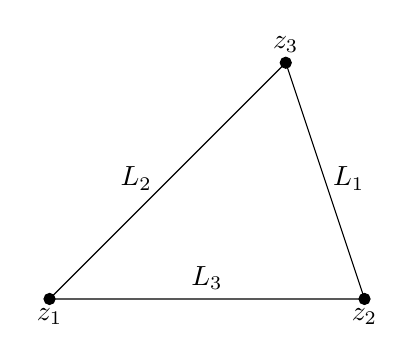
\begin{tikzpicture}[scale=1]
        % 定义三角形的三个顶点
        \coordinate (A) at (0,0);
        \coordinate (B) at (4,0);
        \coordinate (C) at (3,3);
    
        % 绘制三角形
        \draw (A) -- (B) -- (C) -- cycle;
        \node at (3.8,1.8) [anchor=north] {$L_1$};
        \node at (1.1,1.8) [anchor=north] {$L_2$};
        \node at (2,0) [anchor=south] {$L_3$};
    
        % 在每个顶点添加实心圆点
        \filldraw [black] (A) circle (2pt) node[anchor=north] {$z_1$};
        \filldraw [black] (B) circle (2pt) node[anchor=north] {$z_2$};
        \filldraw [black] (C) circle (2pt) node[anchor=south] {$z_3$};
    \end{tikzpicture}
    \caption{$ k=1 $的线性Lagrange元,$ \dim \mathcal{P}_1 = 3 $}
    \label{fig:Lagrange_1}
\end{figure}

当$ k=2 $时,情况是类似的,$ \mathcal{P}_2 $是所有不超过二次的二元多项式构成的空间,于是任意$ P\in \mathcal{P}_2 $都形如
\[
    P(x) = c_0 + c_1 x_1 + c_2 x_2 + c_3 x_1^2 + c_4 x_1x_2 + c_5 x_2^2,
\]
所以$ \dim \mathcal{P}_2 = 6 $,因此根据对偶性为了得到一个有限元需要指定节点变量集$ \mathcal{N}_2 = \{N_1,N_2,N_3,N_4,N_5,N_6\} $。此时的二阶Lagrange元要求节点变量集满足
\begin{equation}
    N_i(v) = v(z_i),\quad i = 1,2,3,4,5,6
\end{equation}
对任意$ v\in \mathcal{P}_2 $都成立,其中$ z_i $是三角形有限元区域$ K $的三个顶点和三条边的中点,如图\ref{fig:Lagrange_2}所示。

\begin{figure}[htpb]
    \centering
    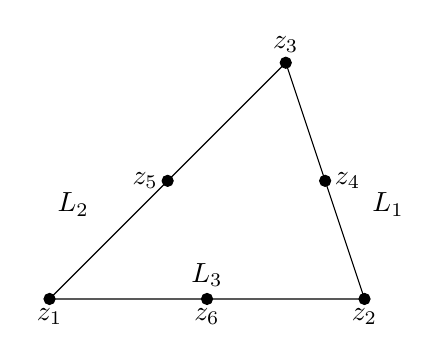
\begin{tikzpicture}[scale=1]
        % 定义三角形的三个顶点
        \coordinate (A) at (0,0);
        \coordinate (B) at (4,0);
        \coordinate (C) at (3,3);
    
        % 绘制三角形
        \draw (A) -- (B) -- (C) -- cycle;
        \node at (4.3,1.2) {$L_1$};
        \node at (0.3,1.2) {$L_2$};
        \node at (2,0.3) {$L_3$};
    
        % 在每个顶点添加实心圆点
        \filldraw [black] (A) circle (2pt) node[anchor=north] {$z_1$};
        \filldraw [black] (B) circle (2pt) node[anchor=north] {$z_2$};
        \filldraw [black] (C) circle (2pt) node[anchor=south] {$z_3$};
        \filldraw [black] (3.5,1.5) circle (2pt) node[anchor=west] {$z_4$};
        \filldraw [black] (1.5,1.5) circle (2pt) node[anchor=east] {$z_5$};
        \filldraw [black] (2,0) circle (2pt) node[anchor=north] {$z_6$};
    \end{tikzpicture}
    \caption{$ k=2 $的Lagrange元,$ \dim \mathcal{P}_2= 6 $}
    \label{fig:Lagrange_2}
\end{figure}

为了说明这一节点变量集$ \mathcal{N}_2 $满足构造有限元的条件,我们需要证明$ \mathcal{N}_2 $确定$ \mathcal{P}_2 $。仍与之前一样设$ L_1,L_2,L_3 $分别是定义了图\ref{fig:Lagrange_2}中三角形$ K $的三条边的线性函数,考虑$ P\in \mathcal{P}_2 $且$ N_i(P) = P(z_i) = 0,i=1,2,3,4,5,6 $的多项式$ P $。因为$ P $是二次多项式但在$ L_1 $所在直线上存在\emph{三个零点},注意到将$ P $限制在$ L_1 $上得到的是一个一元二阶多项式,因此根据代数基本定理$ P $在超平面$ {\rm Ker}\ L_1 $(一条直线)上恒为零。根据引理\ref{lem:polynomial}可知$ P = L_1Q_1 $,其中$ Q_1 $是一个一次多项式。同理,在$ L_2 $和$ L_3 $所在直线上$ P $也具有三个零点,而$ z_1,z_5 $不是$ L_1 $的零点,因此一次多项式$ Q_1 $在$ L_2 $上具有两个零点,于是$ Q_1 $在超平面$ {\rm Ker}\ L_2 $恒为零,再次使用引理\ref{lem:polynomial}可知$ Q_1 = L_2 Q_2 $,其中$ Q_2 $是一个零次多项式,即常数函数$ c $,因此
\[
    P = cL_1L_2.
\]
注意到$ z_6 $既不是$ L_1 $的零点也不是$ L_2 $的零点,然而$ P(z_6)=0 $,所以$ c=0 $,因此$ P \equiv 0 $,于是$ \mathcal{N}_2 $确定$ \mathcal{P}_2 $,$ (K,\mathcal{P}_2,\mathcal{N}_2) $是一个有限元。

为了获得更高阶的Lagrange元,我们可以继续类似的构造,向边界添加更多的节点。

\subsubsection{Hermite元}
换用不同的节点变量集可以得到不同的有限元,Hermite元是另一种常用的三角有限元,我们以$ k=3 $的情况为例介绍Hermite元。此时$ \mathcal{P}_3 $是所有不超过三次的二元多项式构成的空间,于是任意$ P\in \mathcal{P}_3 $都形如
\[
    P(x) = c_0 + c_1 x_1 + c_2 x_2 + c_3 x_1^2 + c_4 x_1x_2 + c_5 x_2^2 + c_6 x_1^3 + c_7 x_1^2x_2 + c_8 x_1x_2^2 + c_9 x_2^3,
\]
所以$ \dim \mathcal{P}_3 = 10 $,因此根据对偶性为了得到一个有限元需要指定节点变量集$ \mathcal{N}_3 = \{N_1,\cdots ,N_{10}\} $。与Lagrange元不同,三阶Hermite元要求节点变量集满足
\begin{equation}
    N_i(v) = v(z_i),\quad i = 1,2,3,4
\end{equation}
且
\begin{equation}
    (N_5(v),N_6(v)) = \nabla v(z_1),\quad (N_7(v),N_8(v)) = \nabla v(z_2),\quad (N_9(v),N_{10}(v)) = \nabla v(z_3).
\end{equation}
当如上条件满足时,$ z_1,z_2,z_3 $在$ N_i(P)=0 $对$ i=1,2,\cdots ,10 $都成立时是三阶多项式$ P $的零点,进一步地,使用导数信息可知$ p $在三条边上均恒为零,另外,$ z_4 $是$ P $的一阶零点。(注意到根据待定系数法将该事实带入$ P $的表示中即可得各阶系数均为零,于是$ P=0 $,以下使用与之前类似的分析也能得到相同的结论)

\begin{figure}[htpb]
    \centering
    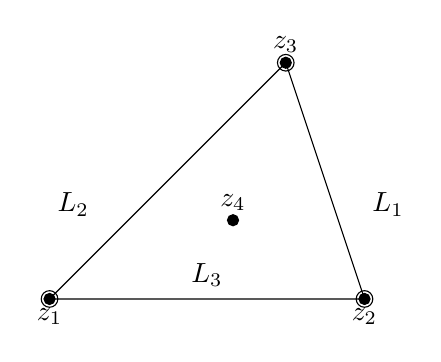
\begin{tikzpicture}[scale=1]
        % 定义三角形的三个顶点
        \coordinate (A) at (0,0);
        \coordinate (B) at (4,0);
        \coordinate (C) at (3,3);
    
        % 绘制三角形
        \draw (A) -- (B) -- (C) -- cycle;
        \node at (4.3,1.2) {$L_1$};
        \node at (0.3,1.2) {$L_2$};
        \node at (2,0.3) {$L_3$};
    
        % 在每个顶点添加实心圆点
        \filldraw [black] (A) circle (2pt) node[anchor=north] {$z_1$};
        \filldraw [black] (B) circle (2pt) node[anchor=north] {$z_2$};
        \filldraw [black] (C) circle (2pt) node[anchor=south] {$z_3$};
        \filldraw [black] (2.33,1) circle (2pt) node[anchor=south] {$z_4$};
        \draw (A) circle (3pt);
        \draw (B) circle (3pt);
        \draw (C) circle (3pt);
    \end{tikzpicture}
    \caption{$ k=3 $的Hermite元,$ \dim \mathcal{P}_2= 10 $}
    \label{fig:Hermite_3}
\end{figure}

为了说明这一节点变量集$ \mathcal{N}_3 $满足构造有限元的条件,我们需要证明$ \mathcal{N}_3 $确定$ \mathcal{P}_3 $。仍与之前一样设$ L_1,L_2,L_3 $分别是定义了图\ref{fig:Hermite_3}中三角形$ K $的三条边的线性函数,考虑$ P\in \mathcal{P}_3 $且$ N_i(P) = P(z_i) = 0,i=1,\cdots ,10 $的多项式$ P $。因为$ P $是三次多项式但在$ L_1 $所在直线上存在两个\emph{二阶零点},注意到将$ P $限制在$ L_1 $上得到的是一个一元三阶多项式,由代数基本定理可知$ P $在超平面$ {\rm Ker}\ L_1 $(一条直线)上恒为零。根据引理\ref{lem:polynomial}可知$ P = L_1Q_1 $,其中$ Q_1 $是一个二次多项式,并且由于$ L_1 $上$ P $有两个二阶零点所以$ z_2,z_3 $中有一个也是$ Q_1 $的根,不妨设为$ z_3 $。在$ L_2 $和$ L_3 $所在直线上$ P $也具有两个二阶零点,而$ z_1 $不是$ L_1 $的零点,因此二次多项式$ Q_1 $在$ L_2 $上具有一个一阶零点$ z_3 $和一个二阶零点$ z_1 $,于是$ Q_1 $在超平面$ {\rm Ker}\ L_2 $恒为零,再次使用引理\ref{lem:polynomial}可知$ Q_1 = L_2 Q_2 $,其中$ Q_2 $是一个一次多项式。同理$ Q_2 = L_3 Q_3 $,其中$ Q_3 $是一个零次多项式,即常数函数$ c $,因此
\[
    P = cL_1L_2L_3.
\]
注意到$ z_4 $既不是$ L_1 $的零点也不是$ L_2 $的零点,然而$ P(z_4)=0 $,所以$ c=0 $,因此$ P \equiv 0 $,于是$ \mathcal{N}_3 $确定$ \mathcal{P}_3 $,$ (K,\mathcal{P}_3,\mathcal{N}_3) $是一个有限元。

\subsection{插值}
有限元方法需要将不同区域上的有限元组装起来以构造出Sobolev空间的有限维子空间,在该子空间中寻找逼近解的函数作为有限元方法的解。上一节我们已经构造了一类有限元,在讨论整体的逼近效果之前,首先应当考虑一个单独的有限元区域上的局部插值的逼近效果。
\begin{definition}
    设$ (K,\mathcal{P},\mathcal{N}) $是一个有限元,$ \{\psi_i\}_{i=1}^k $是与$ \mathcal{N}=\{N_i\}_{i=1}^k $对偶的$ \mathcal{P} $的一组基,任给$ v\in \mathcal{P} $,将$ v $在该有限元上的\textcolor{blue}{局部插值}$ \mathcal{I}_K v $定义为
    \begin{equation}
        \mathcal{I}_K v = \sum_{i=1}^k N_i(v)\psi_i,
    \end{equation}
    局部插值算子$ \mathcal{I}_K: \mathcal{P}\to \mathcal{P} $满足
    \begin{equation}
        \mathcal{I}_K = \sum_{i=1}^k \psi_i N_i.
    \end{equation}
\end{definition}

在一些简单情况下,通过计算$ \psi_i $可以得到局部插值算子的具体形式,例如考虑一阶线性Lagrange元$ (K,\mathcal{P}_1,\mathcal{N}_1) $,由上一节的定义和分析可知$ \mathcal{N}_1 = \{N_1,N_2,N_3\} $满足$ N_i(v) = v(z_i) $,于是
\[
    \mathcal{I}_K v = N_1(v)\psi_1 + N_2(v)\psi_2 + N_3(v)\psi_3 = v(z_1)\psi_1 + v(z_2)\psi_2 + v(z_3)\psi_3,
\]
因此要给出局部插值算子的具体形式只需找到基函数$ \psi_i $。根据对偶性$ N_i(\psi_j) = \delta_{ij} $,因此$ \psi_j(z_i) = \delta_{ij} $。类似于上一节的分析,$ \psi_1\in \mathcal{P}_1 $是线性函数,但是在$ L_1 $上却具有$ z_2,z_3 $两个零点,因此$ \psi_1 = L_1Q_1 $,其中$ Q_1 $是一个常数函数,由于$ \psi_1(z_1) = 1 $,所以$ Q_1 = 1 / L_1(z_1) $,于是$ \psi_1 = L_1/L_1(z_1) $,同理$ \psi_2 = L_2 / L_2(z_2) $,$ \psi_3 = L_3 / L_3(z_3) $,于是
\[
    \mathcal{I}_K v = \frac{v(z_1)L_1}{L_1(z_1)} + \frac{v(z_2)L_2}{L_2(z_2)} + \frac{v(z_3)L_3}{L_3(z_3)}.
\]
其中的$ L_i:\mathbb{R}^2\to \mathbb{R} $是定义了三角形$ K $的三条边的线性函数。考虑最简单的情况,即$ K $是一个单位三角形,三个顶点分别为$ z_1 = (0,0),z_2 = (1,0),z_3 = (0,1) $,则
\[
    L_1(x) = 1-x_1-x_2,\quad L_2(x) = x_2,\quad L_3(x) = x_1,
\]
其中$ x = (x_1,x_2)\in \mathbb{R}^2 $,于是
\[
    (\mathcal{I}_K v)(x) = (1-x_1-x_2)v(0,0) + x_2v(1,0) + x_1v(0,1).
\]

\begin{lemma}
    局部插值满足以下性质:
    \begin{enumerate}
        \item 局部插值算子$ \mathcal{I}_K $是线性的;
        \item 对任意$ v\in \mathcal{P} $,$ N_i(\mathcal{I}_K v) = N_i(v) $;
        \item 对任意$ v\in \mathcal{P} $,$ \mathcal{I}_K v = v $,进而$ \mathcal{I}_K $是$ \mathcal{P} $上的幂等算子(投影算子):$ \mathcal{I}_K^2 = \mathcal{I}_K $。
    \end{enumerate}
\end{lemma}
\noindent 第一条性质是显然的,第二条性质只需要将$ \mathcal{I}_K v $的定义代入$ N_i(\mathcal{I}_K v) $中即可得到,借助前两条性质可得$ N_i(\mathcal{I}_K v - v)=0 $对任意的$ v\in \mathcal{P} $都成立,于是$ \mathcal{I}_K v - v $是$ \mathcal{P} $上的零函数,所以$ \mathcal{I}_K v = v $。

下面我们把不同有限元区域上的局部插值算子组装起来,构造出全局插值算子。首先需要要求区域的划分是合理的,这类合理的划分按如下方式定义。

\begin{definition}
    给定区域$ U $,如果$ U $内存在有限个开子集$ \{K_i\} $满足
    \begin{enumerate}
        \item 当$ i\ne j $时,$ K_i \cap K_j = \varnothing $;
        \item $ \overline{U} = \bigcup_i \overline{K}_i $;
    \end{enumerate}
    则称$ \{K_i\} $是$ U $的一个\textcolor{blue}{细分}(subdivision)。
\end{definition}

之后,把局部插值算子视作同一算子在不同局部的限制,由此定义全局插值算子。

\begin{definition}
    设$ U $是$ \mathbb{R}^n $内的一个有界开集,$ \mathcal{T}=\{K_i\} $是$ U $的一个细分,其中每一个子区域$ K_i $都配备了相应的形状函数空间$ \mathcal{P}_i $和节点变量集$ \mathcal{N}_i $使得$ (K_i,\mathcal{P}_i,\mathcal{N}_i) $是一个有限元。记$ m $为节点变量集的定义中所需的最高阶偏导的阶数。任给$ v\in C^m(\overline{U}) $,定义$ v $在$ U $上的\textcolor{blue}{全局插值}$ \mathcal{I}_h v $满足
    \begin{equation}
        \mathcal{I}_h v|_{K_i} = \mathcal{I}_{K_i} v,\quad \forall K_i\in \mathcal{T}.
    \end{equation}
\end{definition}

在应用中最基本的问题是二维平面上的逼近问题,因此$ U\in \mathbb{R}^2 $的情况值得特别考虑,如上一小节所述,此时最常使用的是三角有限元,因此需要先将$ U $划分为三角形区域。

\begin{definition}
    设$ U $是$ \mathbb{R}^2 $内的一个多边形区域,如果$ U $的细分$ \mathcal{T} $满足
    \begin{enumerate}
        \item 每个$ K_i\in \mathcal{T} $都是一个三角形;
        \item 任一$ K_i\in \mathcal{T} $的顶点都不是$ \mathcal{T} $内其他三角形的非顶点(即$ i\ne j $时$ K_i $的顶点不是$ K_j $边的内点);
    \end{enumerate}
    则称$ \mathcal{T} $是$ U $的一个\textcolor{blue}{三角剖分}(triangulation)。
\end{definition}

当$ v $具有足够的光滑性时,按照如上方法定义的全局插值$ \mathcal{I}_h v $只能保证在各有限元区域内部的连续性,在不同有限元区域之间的连续性不一定可以保持,而通常希望全局插值$ \mathcal{I}_h v $具有尽可能好的光滑性,因此需要对插值算子$ \mathcal{I}_h $的光滑性作进一步的考察。

\begin{definition}
    如果对任意的$ v\in C^m(\overline{U}) $都有$ \mathcal{I}_h v\in C^r(\overline{U}) $,则称$ \mathcal{I}_h $是一个\textcolor{blue}{$ r $阶连续插值算子}(continuity of order $ r $),简记为$ \mathcal{I}_h\in C^r $,并且称
    \begin{equation}
        \{\mathcal{I}_h v:\ v\in C^m(\overline{U})\}
    \end{equation}
    为$ C^r $有限元空间。
\end{definition}
\noindent 该定义没有对$ v $的光滑性阶数$ m $和插值算子$ \mathcal{I}_h $的光滑性阶数$ r $之间的关系作出要求,因此如上定义的$ \mathcal{I}_h $光滑性是借由在被插值函数$ v $\emph{足够光滑}的情况下插值得到的$ \mathcal{I}_hv $的光滑性来定义的。

下面我们说明在三角区域上的Lagrange元和Hermite元的全局插值算子$ \mathcal{I}_h $都是$ C^0 $的。

\begin{theorem}
    三角区域上的Lagrange元和Hermite元的全局插值算子$ \mathcal{I}_h $都是$ C^0 $的。更准确地说,可以通过选取边上的节点变量集构造三角区域上的有限元$ (K,\mathcal{P},\mathcal{N}) $使得$ v\in C^m(\overline{U}) $的全局插值$ \mathcal{I}_h v\in C^0(\overline{U}) $,如果使用Lagrange元则$ m=0 $,如果使用Hermite元则$ m=1 $。
\end{theorem}
\noindent 只需说明在三角区域的边界处的连续性即可,内部的连续性由形状函数的连续性保证。设三角区域$ K_1,K_2 $公用边$ e $,要求$ K_1,K_2 $在$ e $上使用的节点变量的位置相同。令$ w = \mathcal{I}_{K_1}v - \mathcal{I}_{K_2}v $,其中$ \mathcal{I}_{K_i}v $都是阶数不超过$ k $的多项式,我们考虑$ w $在$ e $上的限制。根据Lagrange元和Hermite元对节点变量集的要求,$ e $上具有总阶数超过$ k $的$ w $的零点,所以$ w|_e = 0 $,于是$ \mathcal{I}_{K_1}v $与$ \mathcal{I}_{K_2}v $在$ e $上相等,进而$ \mathcal{I}_h v $在$ e $上连续。

\begin{definition}
    设$ (K,\mathcal{P},\mathcal{N}) $是一个有限元,$ F(x) = Ax+b $是一个仿射变换,其中$ A $是$ n $阶非奇异方阵。如果
    \begin{enumerate}
        \item $ F(K) = \hat{K} $;
        \item $ F^*\hat{\mathcal{P}} = \mathcal{P} $;
        \item $ F_* \mathcal{N} = \hat{\mathcal{N}} $;
    \end{enumerate}
    则称变换后的有限元$ (\hat{K},\hat{\mathcal{P}},\hat{\mathcal{N}}) $与$ (K,\mathcal{P},\mathcal{N}) $\textcolor{blue}{仿射等价}(affine equivalent),其中$ F^* $和$ F_* $是$ F $的拉回和推前算子:
    \begin{equation}
        F^*v = v\circ F,\quad (F_*N)(v) = N(F^*v) = N(v\circ F).
    \end{equation}
\end{definition}
在三角区域上,合适选取节点变量集得到的Larange元之间是互相仿射等价的,类似地,Hermite元之间也是互相仿射等价的。

\subsection{矩形有限元}
除了三角形有限元,矩形有限元也是常用的有限元之一,定义
\begin{equation}
    Q_k = \left\{ \sum_{j}c_j p_j(x)q_j(y):\ p_j , q_j \text{ are polynomials of degree} \leqslant k \right\},
\end{equation}
令$ \mathcal{P}_k^1 $是以不超过$ k $阶的一元多项式组成的空间,则$ \dim Q_k = (\dim \mathcal{P}_k^1)^2 $。矩形有限元的构造与三角形有限元类似,我们以$ k=1 $和$ k=2 $的矩形Lagrange元为例说明。

$ k=1 $时,令$ \mathcal{P} = Q_1 $为形状函数空间,其中的多项式形如
\[
    P(x,y) = (a_0 + a_1 x)(b_0 + b_1 y),
\]
因此$ \dim \mathcal{P} = 4 $。要求节点变量集$ \mathcal{N} = \{N_1,N_2,N_3,N_4\} $满足
\[
    N_i(v) = v(z_i),\quad i = 1,2,3,4,
\]
其中$ z_i $是矩形区域的四个顶点,如图\ref{fig:rectLagrange_1}所示。可以证明$ \mathcal{N} $确定$ \mathcal{P} $,于是$ (K,\mathcal{P},\mathcal{N}) $是一个有限元。

\begin{figure}[htpb]
    \centering
    \begin{tikzpicture}[scale=0.7]
        % 定义三角形的三个顶点
        \coordinate (A) at (0,0);
        \coordinate (B) at (5,0);
        \coordinate (C) at (5,4);
        \coordinate (D) at (0,4);
    
        % 绘制三角形
        \draw (A) -- (B) -- (C) -- (D) -- cycle;
        \node at (5.3,2) {$L_4$};
        \node at (0.3,2) {$L_3$};
        \node at (2.5,4.3) {$L_2$};
        \node at (2.5,0.3) {$L_1$};
    
        % 在每个顶点添加实心圆点
        \filldraw [black] (A) circle (2pt) node[anchor=north] {$z_1$};
        \filldraw [black] (B) circle (2pt) node[anchor=north] {$z_2$};
        \filldraw [black] (C) circle (2pt) node[anchor=south] {$z_3$};
        \filldraw [black] (D) circle (2pt) node[anchor=south] {$z_4$};
    \end{tikzpicture}
    \caption{$ k=1 $的双线性矩形Lagrange元,$ \dim \mathcal{P} = \dim Q_1= 4 $}
    \label{fig:rectLagrange_1}
\end{figure}

$ k=2 $时的情况是类似的,令$ \mathcal{P} = Q_2 $为形状函数空间,其中的多项式形如
\[
    P(x,y) = (a_0 + a_1 x + a_2 x^2)(b_0 + b_1 y + b_2 y^2),
\]
因此$ \dim \mathcal{P} = 9 $。要求节点变量集$ \mathcal{N} = \{N_1,\cdots ,N_9\} $同样满足
\[
    N_i(v) = v(z_i),\quad i = 1,2,\cdots ,9,  
\]
其中$ \{z_i\}_{i=1}^9 $由矩形区域的四个顶点、四条边的中点、以及中心组成,如图\ref{fig:rectLagrange_2}所示。可以证明$ \mathcal{N} $确定$ \mathcal{P} $,于是$ (K,\mathcal{P},\mathcal{N}) $是一个有限元。

\begin{figure}[htpb]
    \centering
    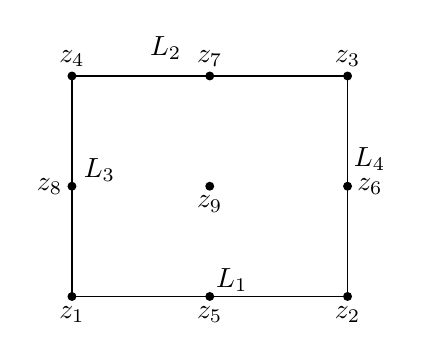
\begin{tikzpicture}[scale=0.7]
        % 定义三角形的三个顶点
        \coordinate (A) at (0,0);
        \coordinate (B) at (5,0);
        \coordinate (C) at (5,4);
        \coordinate (D) at (0,4);
        \coordinate (E) at (2.5,0);
        \coordinate (F) at (5,2);
        \coordinate (G) at (2.5,4);
        \coordinate (H) at (0,2);
        \coordinate (I) at (2.5,2);
    
        % 绘制三角形
        \draw (A) -- (B) -- (C) -- (D) -- cycle;
        \node at (5.4,2.5) {$L_4$};
        \node at (0.5,2.3) {$L_3$};
        \node at (1.7,4.5) {$L_2$};
        \node at (2.9,0.3) {$L_1$};
    
        % 在每个顶点添加实心圆点
        \filldraw [black] (A) circle (2pt) node[anchor=north] {$z_1$};
        \filldraw [black] (B) circle (2pt) node[anchor=north] {$z_2$};
        \filldraw [black] (C) circle (2pt) node[anchor=south] {$z_3$};
        \filldraw [black] (D) circle (2pt) node[anchor=south] {$z_4$};
        \filldraw [black] (E) circle (2pt) node[anchor=north] {$z_5$};
        \filldraw [black] (F) circle (2pt) node[anchor=west] {$z_6$};
        \filldraw [black] (G) circle (2pt) node[anchor=south] {$z_7$};
        \filldraw [black] (H) circle (2pt) node[anchor=east] {$z_8$};
        \filldraw [black] (I) circle (2pt) node[anchor=north] {$z_9$};
    \end{tikzpicture}
    \caption{$ k=2 $的双二次Lagrange元,$ \dim \mathcal{P} = \dim Q_2= 9 $}
    \label{fig:rectLagrange_2}
\end{figure}

\subsection{Sobolev空间中的多项式逼近}
本小节将考虑使用上述方法构造的全局插值函数$ \mathcal{I}_h v $与$ v $在Sobolev空间中的距离,通过使用Hardy-Littlewood极大函数我们可以得到逼近误差的一个可计算的先验上界,这一部分需要较高阶的分析工具。

\subsubsection{Bramble-Hilbert引理}
在这一误差分析中,关键的一步是使用Bramble-Hilbert引理,该引理建立了$ l(v) $与$ v $之间的关系,其中$ l $是Sobolev空间上的合适的有界线性泛函。

\begin{lemma}{\normalfont\bf{(Bramble-Hilbert)}}\label{lem:Bramble-Hilbert}
    给定$ \mathbb{R}^n $上的有界开集$ U $,要求$ U $关于其任意具有正测度的子集$ B $内的任一点都是星型的\footnote{即对任意$ x\in U $而言,$ \{x\}\cup B $的闭凸包都是$ U $的子集}。如果$ l:W^{m,p}(U)\to \mathbb{R} $是一个有界线性泛函,其中$ m\geqslant 1,1<p<\infty $,要求任意至多$ m-1 $阶的多项式$ Q $都满足$ l(Q) = 0 $,则存在常数$ C_1>0 $使得
    \begin{equation}
        \textcolor{red}{|l(v)| \leqslant C_1 |v|_{W^{m,p}(U)}},\quad \forall v\in W^{m,p}(U).
    \end{equation}
\end{lemma}
\begin{proof}
    因为$ l $是$ W^{m,p}(U) $上的有界线性泛函,因此存在$ C_0>0 $使得
    \begin{equation}
        |l(v)| \leqslant C_0 \| v \|_{W^{m,p}(U)},\quad \forall v\in W^{m,p}(U).
    \end{equation}
    又因为存在至多$ m-1 $阶的多项式$ Q $使得$ l(Q) = 0 $,使用线性性可得
    \[
        \begin{aligned}
            |l(v)| = |l(v - Q)| &\leqslant C_0 \| v-Q \|_{W^{m,p}(U)} \\
            &= C_0 \left( \sum_{j=0}^m |v-Q|_{W^{j,p}(U)}^p \right)^{\frac{1}{p}}\\
            &\leqslant C_0 \left( \sum_{j=0}^{m-1} |v-Q|_{W^{j,p}(U)}^p + |v|_{W^{m,p}(U)}^p \right)^{\frac{1}{p}} \\
            &\leqslant C_0 \left( \sum_{j=0}^{m-1} |v-Q|_{W^{j,p}(U)} + |v|_{W^{m,p}(U)} \right).
        \end{aligned}
    \]
    上式中第一个不等式来自于$ l $的有界性,第二个不等关系成立是因为$ Q $的阶数不超过$ m-1 $,而
    \[
        |v|_{W^{k,p}(U)} = \left( \sum_{|\alpha|=k} \| D^\alpha v \|_{L^p(U)}^p \right)^{\frac{1}{p}}  = \left(\sum_{|\alpha|=j} \int_U |D^\alpha v|^p \right)^{\frac{1}{p}},
    \]
    所以$ |v-Q|_{W^{m,p}(U)} = |v|_{W^{m,p}(U)} $。最后第三个不等关系成立是因为括号内的各项都是正的。

    注意到如果对任意的$ v\in W^{j,p}(U) $而言都存在不超过$ m-1 $阶的多项式$ Q $,当$ j=0,1,\cdots ,m-1 $时都存在常数$ K_j>0 $满足
    \begin{equation}\label{eq:ToBeProve}
        |v-Q|_{W^{j,p}(U)} \leqslant  K_j |v|_{W^{m,p}(U)},\quad j=0,1,\cdots ,m-1,
    \end{equation}
    则带入之前的估计可得
    \begin{equation}
        |l(v)| \leqslant C_0(1+K_0+\cdots +K_{m-1})|v|_{W^{m,p}(U)},
    \end{equation}
    因此
    \[
        C_1 = C_0(1+K_0+\cdots +K_{m-1}),
    \]
    引理得证。
\end{proof}

为了完成Bramble-Hilbert引理的证明,我们需要证明式\eqref{eq:ToBeProve}。为此,我们需要引入Hardy-Littlewood极大函数并使用下面的引理。
\begin{lemma}\label{lem:Hardy-Littlewood}
    设$ g\in L^p(\mathbb{R}^n) $,其中$ 1<p<\infty $。给定单位方向向量$ \nu\in \mathbb{R}^n $($ |\nu|=1 $),定义$ g $在$ \nu $方向上的Hardy-Littlewood极大函数为
    \begin{equation}
        g_1(x,\nu) = \sup_{t>0} \frac{1}{t} \int_0^t |g(x+s \nu)|\ ds,
    \end{equation}
    将$ g_1 $关于$ \nu $在单位球面上的$ L^p(\partial B) $范数记为
    \begin{equation}
        g^*(x) = \left( \int_{\partial B:|\nu|=1} |g_1(x,\nu)|^p\ d\sigma_\nu \right)^{\frac{1}{p}},
    \end{equation}
    则$ g^* $与$ g $的$ L^p(\mathbb{R}^n) $范数满足
    \begin{equation}
        \| g^* \|_{L^p(\mathbb{R}^n)} \leqslant \frac{p}{p-1}\omega_n^{1 / p} \| g \|_{L^p(\mathbb{R}^n)},
    \end{equation}
    其中$ \omega_n = 2\pi^{n / 2} / \Gamma(n / 2) $是$ \mathbb{R}^n $内单位球的表面积($ n-1 $维Hausdorff测度),$ \alpha_n = \pi^{n / 2} / \Gamma(n / 2+1) $是单位球的体积($ n $维Lebegues测度)。
\end{lemma}
\begin{proof}
    可以证明以下不等式成立$ ^* $
    \begin{equation}
        \int_{\mathbb{R}^n} g_1(x,\nu)^p \ dx \leqslant \left( \frac{p}{p-1} \right)^p \int_{\mathbb{R}^n} |g(x)|^p\ dx,
    \end{equation}
    于是
    \[
        \begin{aligned}
            \int_{\mathbb{R}^n} |g^*(x)|^p\ dx &= \int_{\mathbb{R^n}}\left( \int_{|\nu|=1}g_1(x,\nu)^p\ d \sigma_v \right)  dx\\
            &= \int_{|\nu|=1} \left( \int_{\mathbb{R}^n} g_1(x,\nu)^p\ dx \right)d\sigma_\nu \\
            &\leqslant \omega_n\left( \frac{p}{p-1} \right)^p \int_{\mathbb{R}^n} |g(x)|^p\ dx.
        \end{aligned}
    \]
    接下来给出$ \omega_n $和$ \alpha_n $的具体表达式。考虑$ \mathbb{R}^n $上的函数$ f(x) = e^{-|x|^2} $,在$ \mathbb{R}^n $内对$ f $的积分为
    \[
        \int_{\mathbb{R}^n} e^{-|x|^2}\ dx = \prod_{i=1}^n \int_{-\infty}^{+\infty} e^{-x_i^2}\ dx_i  = \pi^{n / 2},
    \]
    另一方面使用坐标变换进行球面坐标积分可得
    \[
        \int_{\mathbb{R}^n} e^{-|x|^2}\ dx = \int_0^\infty \int_{\partial B(0,1)} e^{-r^2}\ d\sigma\ r^{n-1}dr  = \int_0^\infty e^{-r^2} \omega_n r^{n-1} dr = \frac{\omega_n}{2} \Gamma(\frac{n}{2}),
    \]
    因此$ \omega_n = 2\pi^{n / 2} / \Gamma(n / 2) $。接着做体积分可得
    \[
        \alpha_n = \int_{B(0,1)} 1\ dx = \int_0^1 \int_{\partial B(0,r)} 1\ d\sigma\ dr = \int_0^1 \omega_n r^{n-1} dr = \frac{\omega_n}{n},
    \]
    所以$ \alpha_n = \pi^{n / 2} / \Gamma(n / 2+1) $。
\end{proof}

下面我们使用上一引理证明式\eqref{eq:ToBeProve}。
\begin{theorem}
    设$ U $是$ \mathbb{R}^n $上的有界开集,$ U $关于其任意具有正测度的子集$ B $内的任一点都是星型的。令$ 1<p<\infty,0\leqslant j<m $,设$ d = \sup_{x,y\in U}|x-y| $是$ U $的直径。如果$ v\in W^{m,p}(U) $,则
    \begin{equation}
        \inf_{Q\in \mathcal{P}_{m-1}} |v-Q|_{W^{j,p}(U)} \leqslant C \frac{d^{m-j+n / p}}{|B|^{1/p}} |v|_{W^{m,p}(U)},
    \end{equation}
    其中$ |B| $为$ B $的$ n $维Lebegues测度,常数$ C $为
    \begin{equation}
        C = \#\{\alpha:|\alpha|=j\}\cdot \frac{m-j}{n^{1 / p}} \frac{p}{p-1} \omega_n^{1 / p}\left( \sum_{|\beta|=m-j} (\beta!)^{-q} \right) ^{1 / q},
    \end{equation}
    这里的$ q = p / (p-1) $是$ p $的共轭指数,$ \#A $表示集合$ A $的基数,$ \beta! = \beta_1!\cdots \beta_n! $。
\end{theorem}
\begin{proof}
    该证明是技术性的。首先,因为光滑函数空间$ C^\infty(\overline{U}) $在$ W^{m,p}(U) $上是稠密的,因此只需证明对任意$ v\in C^\infty(\overline{U}) $定理的结论成立即可,所以以下的证明我们可以对$ v $求任意阶偏导。现在定义
    \begin{eqnarray}
        P_m(v)(x,y) &=& \sum_{|\beta|< m} D^\beta v(x) \frac{(y-x)^\beta}{\beta!},\label{eq:P_m}\\
        Q_m(v)(y) &=& \frac{1}{|B|} \int_B P_m(v)(x,y)\ dx,\label{eq:Q_m}
    \end{eqnarray}
    其中$ x\in B $。注意到这样定义的$ Q_m(v) $是以$ y $为变量的至多$ m-1 $阶的多项式。关于$ |\alpha| $使用归纳法可以证明$ P_m $和$ Q_m $满足
    \begin{equation}
        D^\alpha Q_m(v)(y) = Q_{m-|\alpha|}(D^\alpha v)(y).
    \end{equation}
    现在考察不等式的左端项$ |v-Q_m(v)|_{W^{j,p}(U)} $可得
    \[
        \begin{aligned}
            |v-Q_m(v)|_{W^{j,p}(U)} &= \left( \sum_{|\alpha|=j} \int_U |D^\alpha v - D^\alpha Q_m(v)|^p\ dx \right)^{1 / p} \\
            &= \left( \sum_{|\alpha|=j} \| D^\alpha (v - Q_m(v)) \|^p_{L^p(U)} \right)^{1 / p} \\
            &\leqslant \sum_{|\alpha|=j} \| D^\alpha (v - Q_m(v)) \|_{L^p(U)},
        \end{aligned}
    \]
    因此必须估计$ \| D^\alpha (v - Q_m(v)) \|_{L^p(U)} = \| D^\alpha v - Q_{m-|\alpha|}(D^\alpha v)\|_{L^p(U)} $,其中$ |\alpha|=j $,根据$ Q_m $的定义
    \begin{equation}\label{eq:estimate_0}
        D^\alpha v(y) - Q_{m-j}(D^\alpha v)(y) = \frac{1}{|B|} \int_B D^\alpha v(y) - P_{m-j}(D^\alpha v)(x,y)\ dx.
    \end{equation}
    借助Minkowski不等式
    \[
        \| \int_B u(x,\cdot)dx \|_{L^p(U)} \leqslant  \int_B \| u(x,\cdot) \|_{L^p(U)}\ dx,
    \]
    对\eqref{eq:estimate_0}两侧取$ L^p $范数可得
    \begin{equation}\label{eq:estimate_2}
        \begin{aligned}
            \| D^\alpha v(y) - Q_{m-j}(D^\alpha v)(y) \|_{L^p(U)} 
            &\leqslant \frac{1}{|B|} \int_B \| D^\alpha v(y) - P_{m-j}(D^\alpha v)(x,y) \|_{L^p(U)}\ dx\\
            &= \frac{1}{|B|} \int_B \left( \int_U |D^\alpha v(y) - P_{m-j}(D^\alpha v)(x,y)|^p\ dy \right)^{1 / p} dx.
        \end{aligned}
    \end{equation}
    使用带有\underline{积分形式残差的Taylor定理}$ ^* $可知
    \[
        D^\alpha v(y) - P_{m-j}(D^\alpha v)(x,y) = (m-j)\sum_{|\beta|=m-j} \frac{(y-x)^\beta}{\beta!} \int_0^1 (1-t)^{m-j-1} D^{\alpha+\beta} v(x+t(y-x))\ dt,
    \]
    因为$ |x-y| \leqslant d $,所以
    \[
        \begin{aligned}
            |D^\alpha v(y) - P_{m-j}(D^\alpha v)(x,y)| \leqslant (m-j)d^{m-j} \sum_{|\beta|=m-j} \frac{1}{\beta!} \int_0^1 |D^{\alpha+\beta} v(x+t(y-x))|\ dt,
        \end{aligned}
    \]
    为了标准化$ y-x $以便使用引理\ref{lem:Hardy-Littlewood},使用变量代换$ |y-x|t = s $可得
    \begin{equation}\label{eq:estimate_1}
        |D^\alpha v(y) - P_{m-j}(D^\alpha v)(x,y)| \leqslant (m-j)d^{m-j} \sum_{|\beta|=m-j} \frac{1}{\beta!} \int_0^{|y-x|} |D^{\alpha+\beta} v(x+s\frac{y-x}{|y-x|})|\ \frac{ds}{|y-x|}.
    \end{equation}
    令
    \begin{equation}
        g(x) = 
        \begin{cases}
            \sum_{|\beta|=m-j}\frac{1}{\beta!} |D^{\alpha+\beta} v(x)|, & x\in U,\\
            0, & x\notin U,
        \end{cases}
    \end{equation}
    相应的$ g_1,g^* $分别是按照引理\ref{lem:Hardy-Littlewood}中的方式定义的$ g $在$ y-x $方向上的Hardy-Littlewood极大函数和其在单位球面上的$ L^p $范数,于是可以将\eqref{eq:estimate_1}重写为
    \[
        |D^\alpha v(y) - P_{m-j}(D^\alpha v)(x,y)| \leqslant (m-j)d^{m-j} g_1(x,\frac{y-x}{|y-x|})
    \]
    将上式两侧做$ p $次方并在$ U $上积分并注意到$ U\subset \{(x,y):|x-y|\leqslant d\} $以及$ {\rm supp}\ g = B\subset U $可得
    \[
        \int_U |D^\alpha v(y) - P_{m-j}(D^\alpha v)(x,y)|^p\ dy \leqslant (m-j)^p d^{p(m-j)} \int_{|y-x|\leqslant d} g_1(x,\frac{y-x}{|y-x|})^p\ dy,
    \]
    于是
    \[
        \begin{aligned}
            \left( \int_U |D^\alpha v(y) - P_{m-j}(D^\alpha v)(x,y)|^p\ dy \right) ^{1 / p} 
            &\leqslant (m-j) d^{m-j} \left( \int_0^d \int_{|\nu|=1} g_1(x,\nu)^p\ d \sigma_\nu r^{n-1}dr \right) ^{1 / p} \\
            &= (m-j) d^{m-j} \left( \int_0^dr^{n-1}dr\cdot \int_{|\nu|=1} g_1(x,\nu)^p\ d \sigma_\nu  \right) ^{1 / p}\\
            &= (m-j) d^{m-j+n / p} g^*(x),
        \end{aligned}
    \]
    将这一结果带入\eqref{eq:estimate_2}可得
    \[
        \| D^\alpha v(y) - Q_{m-j}(D^\alpha v)(y) \|_{L^p(U)} \leqslant \frac{1}{|B|}(m-j) d^{m-j+n / p} \int_B g^*(x)\ dx,
    \]
    使用\underline{Hölder不等式}$ ^* $可得
    \[
        \frac{1}{|B|}\int_B g^*(x)\ dx = \frac{1}{|B|}\| g^* \|_{L^1(U)}  \leqslant \frac{1}{|B|^{\frac{1}{p}}} \| g^* \|_{L^p(U)},
    \]
    因此
    \[
        \| D^\alpha v(y) - Q_{m-j}(D^\alpha v)(y) \|_{L^p(U)} \leqslant (m-j) d^{m-j+n / p} |B|^{1-1 / p} \| g^* \|_{L^p(U)}.
    \]
    使用引理\ref{lem:Hardy-Littlewood}中的估计可得
    \[
        \begin{aligned}
            \| D^\alpha v(y) - Q_{m-j}(D^\alpha v)(y) \|_{L^p(U)} &\leqslant \frac{(m-j) d^{m-j+n / p}}{n^{1 / p}|B|^{1 / p}} \frac{p}{p-1} \omega_n^{1 / p} \| g \|_{L^p(\mathbb{R}^n)} \\
            &= \frac{(m-j) d^{m-j+n / p}}{n^{1 / p}|B|^{1 / p}} \frac{p}{p-1} \omega_n^{1 / p} \| g \|_{L^p(U)}.
        \end{aligned}
    \]
    最后还需要根据$ g $的定义将上式中的$ \| g \|_{L^p(U)} $转化为$ v $的范数,注意到
    \[
        \begin{aligned}
            \| g \|_{L^p(U)} 
            &= \| \sum_{|\beta|=m-j}\frac{1}{\beta!} |D^{\alpha+\beta}v| \|_{L^p(U)}\\
            &\leqslant \sum_{|\beta|=m-j} \frac{1}{\beta!} \| D^{\alpha+\beta}v \|_{L^p(U)}\\
            &\leqslant \left( \sum_{|\beta|=m-j} \frac{1}{(\beta!)^q} \right)^{\frac{1}{q}} \cdot \left( \sum_{|\beta|=m-j} \| D^{\alpha+\beta}v \|_{L^p(U)}^p \right)^{\frac{1}{p}},
        \end{aligned}
    \]
    其中$ q = p / (p-1) $,所以
    \[
        \| D^\alpha v(y) - Q_{m-j}(D^\alpha v)(y) \|_{L^p(U)} \leqslant \frac{(m-j) d^{m-j+n / p}p}{n^{1 / p}|B|^{1 / p}(p-1)}  \omega_n^{1 / p} \left[ \sum_{|\beta|=m-j} \frac{1}{(\beta!)^q} \right]^{\frac{1}{q}} \cdot \left[ \sum_{|\beta|=m-j} \| D^{\alpha+\beta}v \|_{L^p(U)}^p \right]^{\frac{1}{p}},
    \]
    将上式代入
    \[
        |v-Q_m(v)|_{W^{j,p}(U)} \leqslant \sum_{|\alpha|=j} \| D^\alpha (v - Q_m(v)) \|_{L^p(U)} = \sum_{|\alpha|=j} \| D^\alpha v - Q_{m-j}(D^\alpha v) \|_{L^p(U)},
    \]
    注意到$ |\alpha|=j $,所以
    \[
        \begin{aligned}
            \sum_{|\alpha|=j}\left( \sum_{|\beta|=m-j} \| D^{\alpha+\beta}v \|_{L^p(U)}^p \right)^{\frac{1}{p}}  
            &\leqslant \sum_{|\alpha|=j}\sum_{|\beta|=m-j} \| D^{\alpha+\beta}v \|_{L^p(U)}\\
            &\leqslant \sum_{|\alpha|=j}|v|_{W^{m,p}(U)}\\
            &\leqslant \#\{\alpha:|\alpha|=j\}\cdot |v|_{W^{m,p}(U)},
        \end{aligned}
    \]
    于是我们最后得到了
    \begin{equation}\label{eq:estimate_3}
        |v-Q_m(v)|_{W^{j,p}(U)} \leqslant C \frac{d^{m-j+n / p}}{|B|^{1/p}} |v|_{W^{m,p}(U)},
    \end{equation}
    这样就证明了定理的结论。
\end{proof}
如果选取$ B $为$ U $内直径为$ \mu d $的开球,其中$ 0<\mu\leqslant 1 $,则
\[
    |B| = \alpha_n (\mu \frac{d}{2})^n = \frac{\omega_n}{n} (\mu \frac{d}{2})^n,
\]
于是在上述定理的条件下,结论变为
\[
    \inf_{Q\in \mathcal{P}_{m-1}} |v-Q|_{W^{j,p}(U)} \leqslant C(m,n,p,j,\mu)d^{m-j} |v|_{W^{m,p}(U)},
\]
其中
\[
    C(m,n,p,j,\mu) = \#\{\alpha:|\alpha|=j\} \frac{(m-j)p}{p-1} \omega_n^{1 / p}(\frac{\mu}{2})^{-n / p}\left( \sum_{|\beta|=m-j} (\beta!)^{-q} \right) ^{1 / q}
\]
是一个与$ d $无关的常数。为了最小化这一常数,应当在保证$ B\subset U $且$ U $关于$ B $内各点都是星型的前提下让$ \mu $尽可能地大。

\subsubsection{先验误差估计}
本小节借助上一小节的结果给出有限元方法的先验误差估计,首先考虑局部插值误差,为了简单起见,可以不失一般性地要求$ K $的直径$ {\rm diam}\ K=1 $,此时如下引理成立。
\begin{lemma}
    考虑有限元$ (K,\mathcal{P},\mathcal{N}) $。如果区域$ K $的直径$ {\rm diam}\ K=1 $,形状函数空间$ \mathcal{P}\subset W^{m,\infty}(K) $,且$ \mathcal{N}\subset (C^\ell(\overline{K}))^* $\footnote{即要求$ \mathcal{N} $内的每个元素都是$ C^\ell(\overline{K}) $上的有界线性泛函,并且$ \mathcal{N} $中的节点变量的定义只涉及到函数的至多$ \ell $阶偏导},则$ 1<p<\infty $时局部插值算子$ \mathcal{I}_h:C^\ell(\overline{K})\to W^{m,p}(K) $是一个\textcolor{red}{有界}线性算子。
\end{lemma}
\begin{proof}
    根据插值算子的定义,对于任意$ v\in C^\ell(\overline{K}) $,有
    \[
        \mathcal{I}_K v = \sum_{i=1}^k N_i(v) \psi_i,
    \]
    其中$ \{\psi_i\}_{i=1}^k $是$ \mathcal{P}(\subset W^{m,\infty}(K)\subset W^{m,p}(K)) $的一组对偶于$ \mathcal{N} $的基函数。对上式两侧求$ W^{m,p}(K) $范数可得
    \[
        \| \mathcal{I}_K v \|_{W^{m,p}(K)} \leqslant \sum_{i=1}^k |N_i(v)| \| \psi_i \|_{W^{m,p}(K)},
    \]
    因为$ N_i:C^\ell(K)\to \mathbb{R} $是有界线性泛函,所以存在常数$ c_i>0 $使得$ |N_i(v)|\leqslant c_i \| v \|_{C^\ell(K)} $,于是
    \[
        \| \mathcal{I}_K v \|_{W^{m,p}(K)} \leqslant \left( \sum_{i=1}^k c_i \| \psi_i \|_{W^{m,p}(K)} \right) \| v \|_{C^\ell(K)},
    \]
    因此$ \mathcal{I}_K $是有界线性算子。
\end{proof}
根据以上引理,可以定义直径为$ 1 $区域上有界的局部插值算子$ \mathcal{I}_K:C^\ell(\overline{K})\to W^{m,p}(U) $的范数为
\begin{equation}
    \sigma(K) = \sup_{{v\in C^\ell(\overline{K})}\backslash \{0\}} \frac{\| \mathcal{I}_K v \|_{W^{m,p}(K)}}{\| v \|_{C^\ell(\overline{K})}}.
\end{equation}
现在我们可以给出局部插值的一个先验误差估计。
\begin{theorem}{\normalfont\textbf{局部插值的先验误差估计}}\label{thm:local_interpolation}
    设$ (K,\mathcal{P},\mathcal{N}) $是满足如下条件的有限元:
    \begin{enumerate}
        \item 有限元区域$ K $关于其任意内部的开球$ B $内的任一点都是星型的;
        \item $ \mathcal{P}_{m-1}\subset \mathcal{P}\subset W^{m,\infty}(K) $;
        \item $ \mathcal{N}\subset (C^\ell(\overline{K}))^* $。
    \end{enumerate}
    如果$ 1<p<\infty $且$ m-\ell-n / p>0 $,则对于任意$ v\in W^{m,p}(K) $和$ 0\leqslant j\leqslant m $都有
    \begin{equation}
        |v-\mathcal{I}_Kv|_{W^{j,p}(K)} \leqslant C(m,n,p,\mu,\sigma(\hat{K}))h^{m-j}_K |v|_{W^{m,p}(K)},
    \end{equation}
    其中$ h_K = {\rm diam}\ K $,$ \hat{K} = \{x / h_K:x\in K\} $,于是$ {\rm diam}\ \hat{K}=1 $满足之前定理的条件,选取$ \mu\in (0,1] $使$ \mu h_K $是在$ K $内最大的开球的直径。
\end{theorem}
\begin{proof}
    不妨设$ K = \hat{K} $已经进行过标准化。根据Sobolev嵌入定理:$ m-\ell> n / p $且$ 1\leqslant p<\infty $时
    \begin{equation}
        W^{m,p}(K) \hookrightarrow C^\ell(\overline{K})
    \end{equation}
    是连续嵌入,$ Id:v\in W^{m,p}(K)\mapsto v\in C^\ell(\overline{K}) $是有界线性算子。根据$ Id $的有界性,存在常数$ C_{m,n,p}>0 $使得任意$ v\in W^{m,p}(K) $都有
    \begin{equation}
        \| v \|_{C^\ell(\overline{K})} \leqslant C_{m,n,p} \| v \|_{W^{m,p}(K)}.
    \end{equation}
    令$ Q_m(v) $是按照\eqref{eq:Q_m}定义的函数
    \[
        Q_m(v)(y) = \frac{1}{|B|}\int_B \sum_{|\beta|<m} D^\beta v(x) \frac{(y-x)^\beta}{\beta!}\ dx,
    \]
    因此$ Q_m(v)(y) $是以$ y $为变量的至多$ m-1 $阶多项式,根据定理的要求$ Q_m(v)\in \mathcal{P}_{m-1}\subset \mathcal{P}\subset W^{m,\infty}(K)\subset W^{m,p}(K) $,而$ \mathcal{I}_K $是到$ \mathcal{P} $的投影算子($ \mathcal{I}_K^2 = \mathcal{I}_K $),所以$ \mathcal{I}_KQ_m(v) = Q_m(v) $。于是
    \[
        \begin{aligned}
            \| v-\mathcal{I}_Kv \|_{W^{m,p}(K)} 
            &\leqslant \| v-Q_m(v) \|_{W^{m,p}(K)} + \| Q_m(v) - \mathcal{I}_Kv \|_{W^{m,p}(K)}\\
            &= \| v-Q_m(v) \|_{W^{m,p}(K)} + \| \mathcal{I}_K(Q_m(v) - v) \|_{W^{m,p}(K)}\\
            &\leqslant \| v-Q_m(v) \|_{W^{m,p}(K)} + \sigma(K) \| Q_m(v) - v \|_{C^\ell(\overline{K})},\\
            &\leqslant (1+ C_{m,n,p}\sigma(K))\| v-Q_m(v) \| _{W^{m,p}(K)}.
        \end{aligned}
    \]
    根据\eqref{eq:estimate_3}可得
    \[
        \begin{aligned}
            \| v-Q_m(v) \|_{W^{m,p}(K)} 
            &= \left( \sum_{j=0}^m |v-Q_m(v)|_{W^{j,p}(K)}^p \right) ^{1 / p} \\
            &\leqslant \sum_{j=0}^m |v-Q_m(v)|_{W^{j,p}(K)}\\
            &\leqslant \sum_{j=0}^m C(m,n,p,j,\mu)h_K^{m-j} |v|_{W^{m,p}(K)}\\
            &= C(m,n,p,\mu) |v|_{W^{m,p}(K)},
        \end{aligned}
    \]
    因为$ h_K=1 $,于是$ C(m,n,p,\mu) = \sum_{j=0}^m C(m,n,p,j,\mu) $。因此对任意$ 0\leqslant j\leqslant m $有
    \[
        |v-\mathcal{I}_Kv|_{W^{j,p}(K)} \leqslant \| v-\mathcal{I}_K v \|_{W^{m,p}(K)}  \leqslant C(m,n,p,\mu,\sigma(\hat{K})) |v|_{W^{m,p}(K)},
    \]
    定理得证,其中$ C(m,n,p,\mu,\sigma(K)) = (1+C_{m,n,p}\sigma(K))C(m,n,p,\mu) $。
\end{proof}

将各处的局部插值估计合起来可以得到全局插值的误差估计。当使用的细分$ \mathcal{T} $足够好时,$ \sigma(K) $可以被$ \mu $控制,定理\ref{thm:local_interpolation}结论中的常数$ C(m,n,p,\mu,\sigma(K)) $可以替换为$ C(m,n,p,\mu) $,此时全局误差可以具有更好的估计。为此需要先定义正则细分(regular subdivision)。
\begin{definition}
    设$ \mathcal{T}=\{K_i\} $是区域$ U $的一个细分,如果存在$ \mu>0 $使得任意$ K\in \mathcal{T} $都有
    \begin{equation}
        \mu h_K \leqslant \rho_K \leqslant h_K,
    \end{equation}
    其中$ h_K = {\rm diam}\ K $,$ \rho_K $是$ K $内最大的开球的半径,则称$ \mathcal{T} $是一个正则细分。
\end{definition}

考虑互相仿射等价的两个有限元$ (K,\mathcal{P},\mathcal{N}) $和$ (\hat{K},\hat{\mathcal{P}},\hat{\mathcal{N}}) $,两者之间的仿射变换为
\[
    x\mapsto \hat{x} = F(x) = Ax+b,
\]
其中$ A = (a_{ij})_{n\times n} $,记$ A^{-1} $中的元素为$ a^{(-1)}_{ij} $,则根据仿射等价的定义
\[
    F^*\hat{\mathcal{P}} = \mathcal{P},\quad F_*\mathcal{N} = \hat{\mathcal{N}},
\]
所以
\[
    \psi_i(x) = F^* \hat{\psi}_i(x)= \hat{\psi}_i(F(x)) = \hat{\psi}_i(\hat{x}),\quad \hat{N}_i(\hat{v}) = (F_*N_i)\hat{v} = N_i(F^*\hat{v}) = N_i(\hat{v}\circ F),
\]
于是$ (\hat{K},\hat{\mathcal{P}},\hat{\mathcal{N}}) $上的局部插值算子为
\[
    \hat{\mathcal{I}}_{\hat{K}}\hat{v}(\hat{x}) = \sum_{i=1}^k \hat{N}_i(\hat{v})\hat{\psi}_i(\hat{x}) = \sum_{i=1}^k (F_*N_i)\hat{v}(F^{-1})^*\psi_i(\hat{x}),
\]
因为$ (F_*N_i)\hat{v} = N_i(\hat{v}\circ F) $,使用$ N_i $和$ F $的有界性可得
\[
    \begin{aligned}
        |(F_*N_i)\hat{v}|\leqslant C_i \| F^* \hat{v} \|_{C^\ell(\overline{K})}.
    \end{aligned}
\]
又因为$ F^*\hat{v}(x) = \hat{v}(F(x)) = \hat{v}(\hat{x}) $,所以
\[
    \begin{aligned}
        \| F^* \hat{v} \|_{C^\ell(\overline{K})} = \sup_{\| x \|=1} |\hat{v}(\hat{x})|
        = \sup_{\| x \|=1} |\hat{v}(F(x))|
        &\leqslant \sup_{\| x \|=1} \frac{|\hat{v}(\hat{x})|}{\| \hat{x} \| }\cdot \| F(x) \|\\
        &\leqslant \sup_{\| x \|=1} \frac{|\hat{v}(\hat{x})|}{\| \hat{x} \| }\cdot \sup_{\| x \|=1} \| F(x) \|\\
        &\leqslant \sup_{\hat{x}\ne 0} \frac{|\hat{v}(\hat{x})|}{\| \hat{x} \| } \cdot \sup_{\| x \|=1} \| Ax+b \|\\
        &= \| \hat{v} \|_{C^\ell(\overline{\hat{K}})}\cdot \sup_{\| x \|=1} \| Ax+b \|,
    \end{aligned}
\]
进而$ ^* $
\begin{equation}
    |(F_*N_i)\hat{v}| \leqslant C_{i,n,\ell} \left( 1+\max_{1\leqslant i,j\leqslant n}|a_{ij}| \right)^\ell \| \hat{v} \|_{C^\ell(\overline{\hat{K}})},
\end{equation}
类似地
\begin{equation}
    \| (F^{-1})^*\psi_i \|_{W^{m,p}(\hat{K})} \leqslant C_{i,n,m}' \left( 1+\max_{1\leqslant i,j\leqslant n}|a^{(-1)}_{ij}| \right)^m|\det(A)|^{1 / p} \| \psi_i \|_{W^{m,p}(K)},
\end{equation}
至此我们可以估计仿射变换后$ \hat{\mathcal{I}}_{\hat{K}} $的算子范数$ \sigma(\hat{K}) $:
\begin{equation}
    \| \hat{\mathcal{I}}_{\hat{K}} \hat{v} \|_{W^{m,p}(\hat{K})} \leqslant C_{\rm ref}\left( 1+\max_{1\leqslant i,j\leqslant n}|a_{ij}| \right)^\ell \left( 1+\max_{1\leqslant i,j\leqslant n}|a^{(-1)}_{ij}| \right)^m|\det(A)|^{1 / p}\| \hat{v} \|_{C^\ell(\overline{\hat{K}})},
\end{equation}
其中
\[
    C_{\rm ref} = k \max_{i=1,2,\cdots ,k}\{C_{i,n,\ell}\}\max_{i=1,2,\cdots ,k}\{C_{i,n,m}'\}\max_{i=1,2,\cdots ,k}\{\| \psi_i \|_{W^{m,p}(K)} \},
\]
$ k=\dim \mathcal{P} $是$ \mathcal{N} $中元素的个数。感觉算子范数的定义,$ \sigma(\hat{K}) $满足如下估计:
\begin{equation}
    \sigma(\hat{K}) \leqslant C_{\rm ref}\left( 1+\max_{1\leqslant i,j\leqslant n}|a_{ij}| \right)^\ell \left( 1+\max_{1\leqslant i,j\leqslant n}|a^{(-1)}_{ij}| \right)^m|\det(A)|^{1 / p}.
\end{equation}

当使用的细分$ \mathcal{T} $是正则的时,根据如上估计可以证明存在不依赖于$ \hat{K}\in \mathcal{T} $的常数$ C_\mu $使得
\[
    \sigma(\hat{K}) \leqslant C_\mu.
\]
于是定理\ref{thm:local_interpolation}内的局部插值的先验误差估计可以得到改进
\begin{equation}
    |v-\mathcal{I}_Kv|_{W^{j,p}(K)} \leqslant C(m,n,p,\mu)h_K^{m-j} |v|_{W^{m,p}(K)},
\end{equation}
进而在定理\ref{thm:local_interpolation}的条件下对于全局插值算子$ \mathcal{I} $有\textcolor{red}{全局误差估计}
\begin{equation}
    \left( \sum_{K\in \mathcal{T}}h_K^{(j-m)p}|v-\mathcal{I}_Kv|_{W^{j,p}(K)}^p \right)^{1 / p} \leqslant C(m,n,p,\mu) |v|_{W^{m,p}(U)}.
\end{equation}
其中$ v\in W^{m,p}(U) $。特别地,如果令$ h = \max_{K\in \mathcal{T}}h_K $,则上述全局误差估计变为
\begin{equation}
    \textcolor{red}{|v-\mathcal{I}_hv|_{W^{j,p}(U)} \leqslant C(m,n,p,\mu)h^{m-j} |v|_{W^{m,p}(U)}},\quad j=0,1,\cdots ,m.
\end{equation}

\subsubsection{最优误差界}
现在考虑使用$ H^1 $范数对插值误差进行估计。以二阶椭圆方程的零边值问题为例,根据Céa引理其有限元近似解$ u_h\in V_h\subset H^1_0(U) $满足
\begin{equation}
    \| u-u_h \|_{H^1(U)} \leqslant \frac{c_1}{c_0}\inf_{v_h\in V_h} \| u-v_h \|_{H^1(U)}.
\end{equation}
当使用分片线性函数作为形状函数且区域为$ U=(0,1)\times (0,1) $时,如果弱解$ u\in H^2(U)\cap H^1_0(U) $,则
\[
    \| u-u_h \|_{H^1(U)} \leqslant C h | u |_{H^2(U)}.
\]
更一般地,当使用分片多项式作为形状函数且区域细分正则时,可以选取近似空间为
\[
    V_h = \mathcal{I}_h(H^m(U)\cap H^1_0(U)),
\]
于是当弱解$ u\in H^m(U)\cap H^1_0(U) $时,借助上一节的全局误差估计可得
\begin{equation}
    \inf_{v_h\in V_h} \| u-v_h \|_{H^1(U)} \leqslant \| u-\mathcal{I}_hv \|_{H^1(U)}\leqslant C(m,n,\mu) h^{m-1} | u |_{H^m(U)},
\end{equation}
进而
\begin{equation}
    \| u-u_h \|_{H^1(U)} \leqslant C(m,n,\mu,c_1,c_0) h^{m-1} | u |_{H^m(U)}.
\end{equation}
这一结果表明,当使用$ m-1 $阶分片多项式作为形状函数且$ u\in H^m(U) $时,$ H^1 $范数下的插值误差大小为$ O(h^{m-1}) $。因为对于这一问题当给定阶数$ m $时能得到的最优误差界为$ O(h^{m-1}) $,所以这一插值误差估计上界称为最优误差上界。

\section{后验误差估计}
以上得到的所有误差估计都是在实际计算有限元解$ u_h $之前就可以得到的,误差界中不涉及$ u_h $,这些误差估计称为\emph{先验误差估计},本节我们以一维问题为例介绍一种在得到计算结果之后,借助有限元解$ u_h $来估计误差$ \| u-u_h \| $的方法,这种误差估计称为\emph{后验误差估计}。

考虑如下两点边值问题$ (D) $:
\[
    \begin{aligned}
        -u''(x) + b(x)u'(x) + c(x)u(x) &= f(x),\quad x\in (0,1),\\
        u(0) &= 0,\quad u(1) = 0,
    \end{aligned}  
\]
其中$ b\in W^{1,\infty}(I),c\in L^\infty(I),f\in L^2(I) $,该问题在$ c-\frac{1}{2}b'\geqslant 0 $时满足强制性要求,且相应的$ a,l $有界,于是根据Lax-Milgram定理该问题有唯一弱解$ u\in H^1_0(I) $。和往常一样构造变分问题$ (V) $和有限元问题$ (V_h) $。

现在我们定义辅助问题$ (A) $:
\begin{equation}
    \begin{aligned}
        -w''(x) \textcolor{blue}{-[b(x)w(x)]'}+ c(x)w(x) &= \textcolor{blue}{u(x)-u_h(x)},\quad x\in (0,1),\\
        w(0) &= 0,\quad w(1) = 0,
    \end{aligned}
\end{equation}
为原问题的\emph{对偶问题}或\emph{伴随问题},其中$ u,u_h $分别原问题的弱解和有限元解。设$ w $为该对偶问题的弱解,则
\[
    \begin{aligned}
        \| u - u_h \|_{L^2(I)}^2 = (u-u_h,u-u_h) 
        &= (u-u_h,\textcolor{red}{-w''(x) -[b(x)w(x)]'+ c(x)w(x)})\\
        &= a(u-u_h,w),
    \end{aligned}
\]
其中
\[
    a(u,v) = \int_I (u'v'+bu'v+cuv)\ dx = \int_I (u'v'+u(bv)'+cuv)\ dx.
\]
因为$ a $具有Galerkin正交性,即
\[
    a(u-u_h,w_h) = 0,\quad \forall w_h\in V_h,
\]
令$ w_h = \mathcal{I}_h w $为$ w $在$ V_h $上的线性插值,于是
\[
    a(u-u_h,\mathcal{I}_h w) = 0,
\]
进而
\[
    \begin{aligned}
        \| u - u_h \|_{L^2(I)}^2 = a(u-u_h,w-\mathcal{I}_h w) 
        &= a(u,w-\mathcal{I}_h w) - a(u_h,w-\mathcal{I}_h w)\\
        &= l(w-\mathcal{I}_h w) - a(u_h,w-\mathcal{I}_h w),
    \end{aligned}
\]
在上式中已经将未知的弱解$ u $消去了,现在只需要分别估计$ l(w-\mathcal{I}_h w) $和$ a(u_h,w-\mathcal{I}_h w) $的大小即可得到一个与$ u $无关的误差估计。

首先考虑$ l(w-\mathcal{I}_h w) $,根据$ l $的定义可得
\[
    l(w-\mathcal{I}_h w) = (f,w-\mathcal{I}_h w) = \sum_{i=1}^{N}\int_{x_{i-1}}^{x_i} f(x)(w(x)-\mathcal{I}_h w(x))\ dx.
\]
另一方面,根据$ a $的定义可得
\[
    \begin{aligned}
        a(u_h,w-\mathcal{I}_h w) 
        &= \int_I (u_h'(w-\mathcal{I}_h w)'-bu_h'(w-\mathcal{I}_h w)+cu_h(w-\mathcal{I}_h w))\ dx\\
        &= \sum_{i=1}^{N}\int_{x_{i-1}}^{x_i} [-u''_h(x)+b(x)u_h'(x)+c(x)u_h(x)](w(x)-\mathcal{I}_h w(x))\ dx,
    \end{aligned}
\]
所以
\begin{equation}
    \| u - u_h \|_{L^2(I)}^2 = \sum_{i=1}^{N}\int_{x_{i-1}}^{x_i} R(u_h)(w-\mathcal{I}_hw)\ dx,
\end{equation}
其中
\begin{equation}
    R(u_h)(x) = f(x) - [-u''_h(x)+b(x)u_h'(x)+c(x)u_h(x)],\quad x\in (x_{i-1},x_i)
\end{equation}
称为有限元残差。使用Cauchy-Schwarz不等式可得
\[
    \| u - u_h \|_{L^2(I)}^2 \leqslant \sum_{i=1}^{N}\| R(u_h) \|_{L^2(x_{i-1},x_i)}\| w-\mathcal{I}_h w \|_{L^2(x_{i-1},x_i)},
\]
而借助之前的插值误差估计
\[
    \| w-\mathcal{I}_h w \|_{L^2(x_{i-1},x_i)} \leqslant \left( \frac{h_i}{\pi} \right)^2  | w |_{H^2(I_i)},
\]
因此
\begin{equation}
    \| u - u_h \|^2_{L^2(I)} \leqslant \frac{1}{\pi^2}\sum_{i=1}^{N}h_i^2 \| R(u_h) \|_{L^2(x_{i-1},x_i)}| w |_{H^2(I_i)},
\end{equation}
使用均值不等式可得
\begin{equation}
    \begin{aligned}
        \| u - u_h \|^2_{L^2(I)} 
        &\leqslant \frac{1}{\pi^2}\left( \sum_{i=1}^{N}h_i^4 \| R(u_h) \|_{L^2(x_{i-1},x_i)}^2 \right)^{1 / 2}\left( \sum_{i=1}^{N} | w |_{H^2(I_i)}^2 \right)^{1 / 2} \\
        &= \frac{1}{\pi^2}\left( \sum_{i=1}^{N}h_i^4 \| R(u_h) \|_{L^2(x_{i-1},x_i)}^2 \right)^{1 / 2}| w |_{H^2(I)}.
    \end{aligned}
\end{equation}
为了得到最终的估计,接下来我们需要消去上式中未知的$ | w |_{H^2(I)} = \| w'' \|_{L^2(I)} $。

由对偶问题可知
\[
    w'' = -[b(x)w(x)]' + c(x)w(x) + u_h(x) - u(x) = (u_h - u) - bw' + (c-b')w,
\]
于是
\[
    \| w'' \|_{L^2(I)} \leqslant \| u_h - u \|_{L^2(I)} + \| b \|_{L^\infty(I)} \| w' \|_{L^2(I)} + \| c-b' \|_{L^\infty(I)}\| w \|_{L^2(I)}.
\]
现在我们使用$ \| u-u_h \|_{L^2(I)} $来控制$ \| w' \|_{L^2(I)} $和$ \| w \|_{L^2(I)} $进而控制$ | w |_{H^2(I)} $。根据$ (A) $的定义可得
\[
    (u-u_h,w) = (w, -w'' + (bw)' - c'w),
\]
展开上式右侧可得
\[
    \begin{aligned}
        (w, -w'' + (bw)' - cw) 
        &= \| w' \|_{L^2(I)}^2 - \int_I bww'\ dx - \int_I cww\ dx\\
        &= \| w' \|_{L^2(I)}^2 + \int_I \frac{1}{2}b(w^2)'\ dx-\int_Icw^2\ dx\\
        &= \| w' \|_{L^2(I)}^2 + \int_I \frac{1}{2}b'w^2\ dx-\int_Icw^2\ dx\\
        &= \| w' \|_{L^2(I)}^2 + \int_I (\frac{1}{2}b'-c)w^2\ dx,
    \end{aligned}
\]
所以
\[
    (u-u_h,w) = \| w' \|_{L^2(I)}^2 + \int_I (\frac{1}{2}b'-c)w^2\ dx,
\]
因为要求$ c-\frac{1}{2}b'\geqslant 0 $以保证强制性,所以
\begin{equation}
    \| w' \|_{L^2(I)}^2 \leqslant (u-u_h,w)  \leqslant \| u-u_h \|_{L^2(I)} \| w \|_{L^2(I)},
\end{equation}
又根据Poincaré不等式$ \| w \|_{L^2(I)}^2 \leqslant \frac{1}{2}\| w' \|_{L^2(I)}^2 $,带入上式可得
\begin{equation}
    \| w' \|_{L^2(I)} \leqslant \frac{1}{\sqrt{2} }\| u-u_h \|_{L^2(I)},
\end{equation}
进而
\begin{equation}
    \| w \|_{H^1(I)} \leqslant \frac{1}{\sqrt{2}}\| w' \|_{L^2(I)} \leqslant \frac{1}{2}\| u-u_h \|_{L^2(I)},
\end{equation}
所以
\begin{equation}
    | w |_{H^2(I)} \leqslant (1+\frac{1}{\sqrt{2}}\| b \|_{L^\infty(I)}+\frac{1}{2}\| c-b' \|_{L^\infty(I)})\| u-u_h \|_{L^2(I)},
\end{equation}
至此我们得到了后验误差估计的最终形式
\begin{equation}
    \| u - u_h \|_{L^2(I)} \leqslant \frac{1+\frac{1}{\sqrt{2}}\| b \|_{L^\infty(I)}+\frac{1}{2}\| c-b' \|_{L^\infty(I)}}{\pi^2}\left( \sum_{i=1}^{N}h_i^4 \| R(u_h) \|_{L^2(x_{i-1},x_i)}^2 \right)^{1 / 2},
\end{equation}
这一估计的右侧不包含未知的弱解$ u $,只与有限元解$ u_h $有关,所以这一估计称为后验误差估计。如果令$ h=\max_i h_i $,则
\begin{equation}
    \| u - u_h \|_{L^2(I)} \leqslant \frac{1+\frac{1}{\sqrt{2}}\| b \|_{L^\infty(I)}+\frac{1}{2}\| c-b' \|_{L^\infty(I)}}{\pi^2}\left( \sum_{i=1}^{N}\| R(u_h) \|_{L^2(x_{i-1},x_i)}^2 \right)^{1 / 2}h^2,
\end{equation}
所以这一后验误差估计的误差界为$ O(h^2) $。

\end{document}